This chapter provides the results of the different approaches that have been used during the evaluation phase. First, the results of the Exploration Algorithm are presented. The test cases were all done visually using Python plots as described in section \ref{sec:Visual Verification with Plots}. Second, the results of the Optimization Algorithm are presented. Again, the test cases are outputted visually using Python plots as described in section \ref{sec:Visual Verification with Plots}. Additionally, each track's calculation times and estimated lap times were calculated. In the end, the integration tests with both algorithms are presented using the Simulation Tool.

\section{Exploration Algorithm Specifics} \label{sec:Exploration Algorithm Specifics}
The exploration algorithm tests were done using Python plots. Track information like cone positions and the starting position of the car were loaded from the track files by the \acrlong{tum}. \cite{tumftm_optimization_algoritm} Additionally, each algorithm cycle and the total algorithm calculation time were observed.

Different config parameters for the thresholds had to be loaded for each track for the Exploration Algorithm, as the scale of the tracks were not similar. The different parameters are the starting position of the car on the track, the position distance threshold (maximum distance a newly received cone can have with the car's current position), the cone distance threshold (maximum distance nearby cones can have with the newly received cone, to be considered for triangulation), the cone threshold (minimum number of cones for triangulation) and the edges distance threshold (maximum length an edge can have to be considered for middle point calculation). The default parameters for the Exploration Algorithm are given as follows in table \ref{tab:Default Track Config for Exploration Algorithm}:
\begin{table}[H]
    \centering
    \begin{tabular}{|l|l|l|}
        \hline
        \textbf{Config Parameter}     & \textbf{Value} \\ \hline
        START\_CURRENT\_POSITION      & [0.0, 0.0]     \\ \hline
        POSITION\_DISTANCE\_THRESHOLD & 20 m           \\ \hline
        CONE\_DISTANCE\_THRESHOLD     & 12 m           \\ \hline
        CONES\_THRESHOLD              & 3              \\ \hline
        EDGE\_DISTANCE\_THRESHOLD     & 7 m            \\ \hline
    \end{tabular}
    \caption{Current default track configuration parameters. They are subject to change after further testing.}
    \label{tab:Default Track Config for Exploration Algorithm}
\end{table}

\section{Optimization Algorithm Specifics}
The Optimization Algorithm makes use of many parameters. A GGV diagram (performance envelope) showing the maximum acceleration the car can sustain in any horizontal direction when travelling at any speed. Furthermore, an 'Ax Machines Array' containing an array with the longitudinal acceleration limits by the electrical motors, among other things. The default data for the GGV diagram is shown in table \ref{tab:GGV Diagram}, while the default data for the 'Ax Machines Array' is shown in table \ref{tab:Ax Machines Array}. As both of those have not yet been recorded for the actual race car of \acrshort{zur}, the default data provided by \acrshort{tumftm} has been used.

\begin{table}[H]
    \centering
    \begin{tabular}{|l|l|l|}
        \hline
        \textbf{v\_mps} & \textbf{ax\_max\_mps2} & \textbf{ay\_max\_mps2} \\ \hline
        0.0             & 12.0                   & 12.0                   \\ \hline
        4.0             & 12.0                   & 12.0                   \\ \hline
        8.0             & 12.0                   & 12.0                   \\ \hline
        12.0            & 12.0                   & 12.0                   \\ \hline
        16.0            & 12.0                   & 12.0                   \\ \hline
        20.0            & 12.0                   & 12.0                   \\ \hline
        24.0            & 12.0                   & 12.0                   \\ \hline
        28.0            & 12.0                   & 12.0                   \\ \hline
        32.0            & 12.0                   & 12.0                   \\ \hline
        36.0            & 12.0                   & 12.0                   \\ \hline
        40.0            & 12.0                   & 12.0                   \\ \hline
        44.0            & 12.0                   & 12.0                   \\ \hline
        48.0            & 12.0                   & 12.0                   \\ \hline
        52.0            & 12.0                   & 12.0                   \\ \hline
        56.0            & 12.0                   & 12.0                   \\ \hline
        60.0            & 12.0                   & 12.0                   \\ \hline
        64.0            & 12.0                   & 12.0                   \\ \hline
        68.0            & 12.0                   & 12.0                   \\ \hline
        72.0            & 12.0                   & 12.0                   \\ \hline
    \end{tabular}
    \caption{The supplied GGV diagram (``ggv.csv''), also known as the performance envelope, shows the maximum acceleration the car can sustain in any horizontal direction when travelling at any speed.}
    \label{tab:GGV Diagram}
\end{table}

\begin{table}[H]
    \centering
    \begin{tabular}{|l|l|l|}
        \hline
        \textbf{v\_mps} & \textbf{ax\_max\_machines\_mps2} \\ \hline
        0.0             & 5.3                              \\ \hline
        4.0             & 5.3                              \\ \hline
        8.0             & 5.3                              \\ \hline
        12.0            & 5.3                              \\ \hline
        16.0            & 5.3                              \\ \hline
        20.0            & 5.3                              \\ \hline
        24.0            & 5.3                              \\ \hline
        28.0            & 5.3                              \\ \hline
        32.0            & 5.3                              \\ \hline
        36.0            & 5.3                              \\ \hline
        40.0            & 5.1                              \\ \hline
        44.0            & 5.0                              \\ \hline
        48.0            & 4.6                              \\ \hline
        52.0            & 4.1                              \\ \hline
        56.0            & 3.7                              \\ \hline
        60.0            & 2.7                              \\ \hline
        66.0            & 2.2                              \\ \hline
        72.0            & 1.5                              \\ \hline
    \end{tabular}
    \caption{The supplied ``ax\_max\_machines.csv'', containing an array with the longitudinal acceleration limits by the electrical motors.}
    \label{tab:Ax Machines Array}
\end{table}

Furthermore, additional options have been used with the Optimization Algorithm, those being step size options, spline regression smooth options, velocity profile calculation options, specific optimization problem options, and the general vehicle parameters. Excluding the general vehicle parameters, the set options are:
\begin{itemize}
    \item Step Size options
          \begin{itemize}
              \item Step Size Prep: 1.0 m (used for linear interpolation before spline approximation)
              \item Step Size Reg: 3.0 m (used for spline interpolation after spline approximation during optimization)
              \item Step Size Interp: 2.0 m (used for spline interpolation after optimization)
          \end{itemize}
    \item Spline Regression Smooth options
          \begin{itemize}
              \item K: 3 (order of B-Splines)
              \item S: 10 (smoothing factor ranging from 1.0 to 100.0)
          \end{itemize}
    \item Velocity Profile Calculation options
          \begin{itemize}
              \item Dyn Model Exp: 1.0 (exponents used in the vehicle dynamics model ranging from 1.0 to 2.0)
              \item Conv Filt Window: not used (moving average filter window size for velocity profile)
          \end{itemize}
    \item Optimization Problem Options
          \begin{itemize}
              \item Width Opt: 2.6 m (Vehicle Width for Optimization including Safety Distance)
              \item IQP Iters Min: 3 (minimum number of iterations for IQP)
              \item IQP Curv Error Allowed: 0.01 rad/m (maximum allowed curvature error for IQP)
          \end{itemize}
\end{itemize}

As it goes for the general vehicle parameters, the real specifications of the \acrshort{zur} race car have been provided and are listed in table \ref{tab:ZUR Vehicle Specifications}. The car is shown in figure \ref{fig:ZUR Racecar 2}.
\begin{table}[H]
    \centering
    \begin{tabular}{|l|l|l|}
        \hline
        \textbf{Parameter}    & \textbf{Value} \\ \hline
        Maximal Vehicle Speed & 30.61 m/s      \\ \hline
        Vehicle Length        & 2.931 m        \\ \hline
        Vehicle Width         & 1.663 m        \\ \hline
        Vehicle Mass          & 255.0 kg       \\ \hline
        Drag Coefficient      & 0.3 kg*m2/m3   \\ \hline
        Curvature Limit       & 0.33 rad/m     \\ \hline
    \end{tabular}
    \caption{The specifications of the vehicle.}
    \label{tab:ZUR Vehicle Specifications}
\end{table}
\begin{figure}[H]
    \centering
    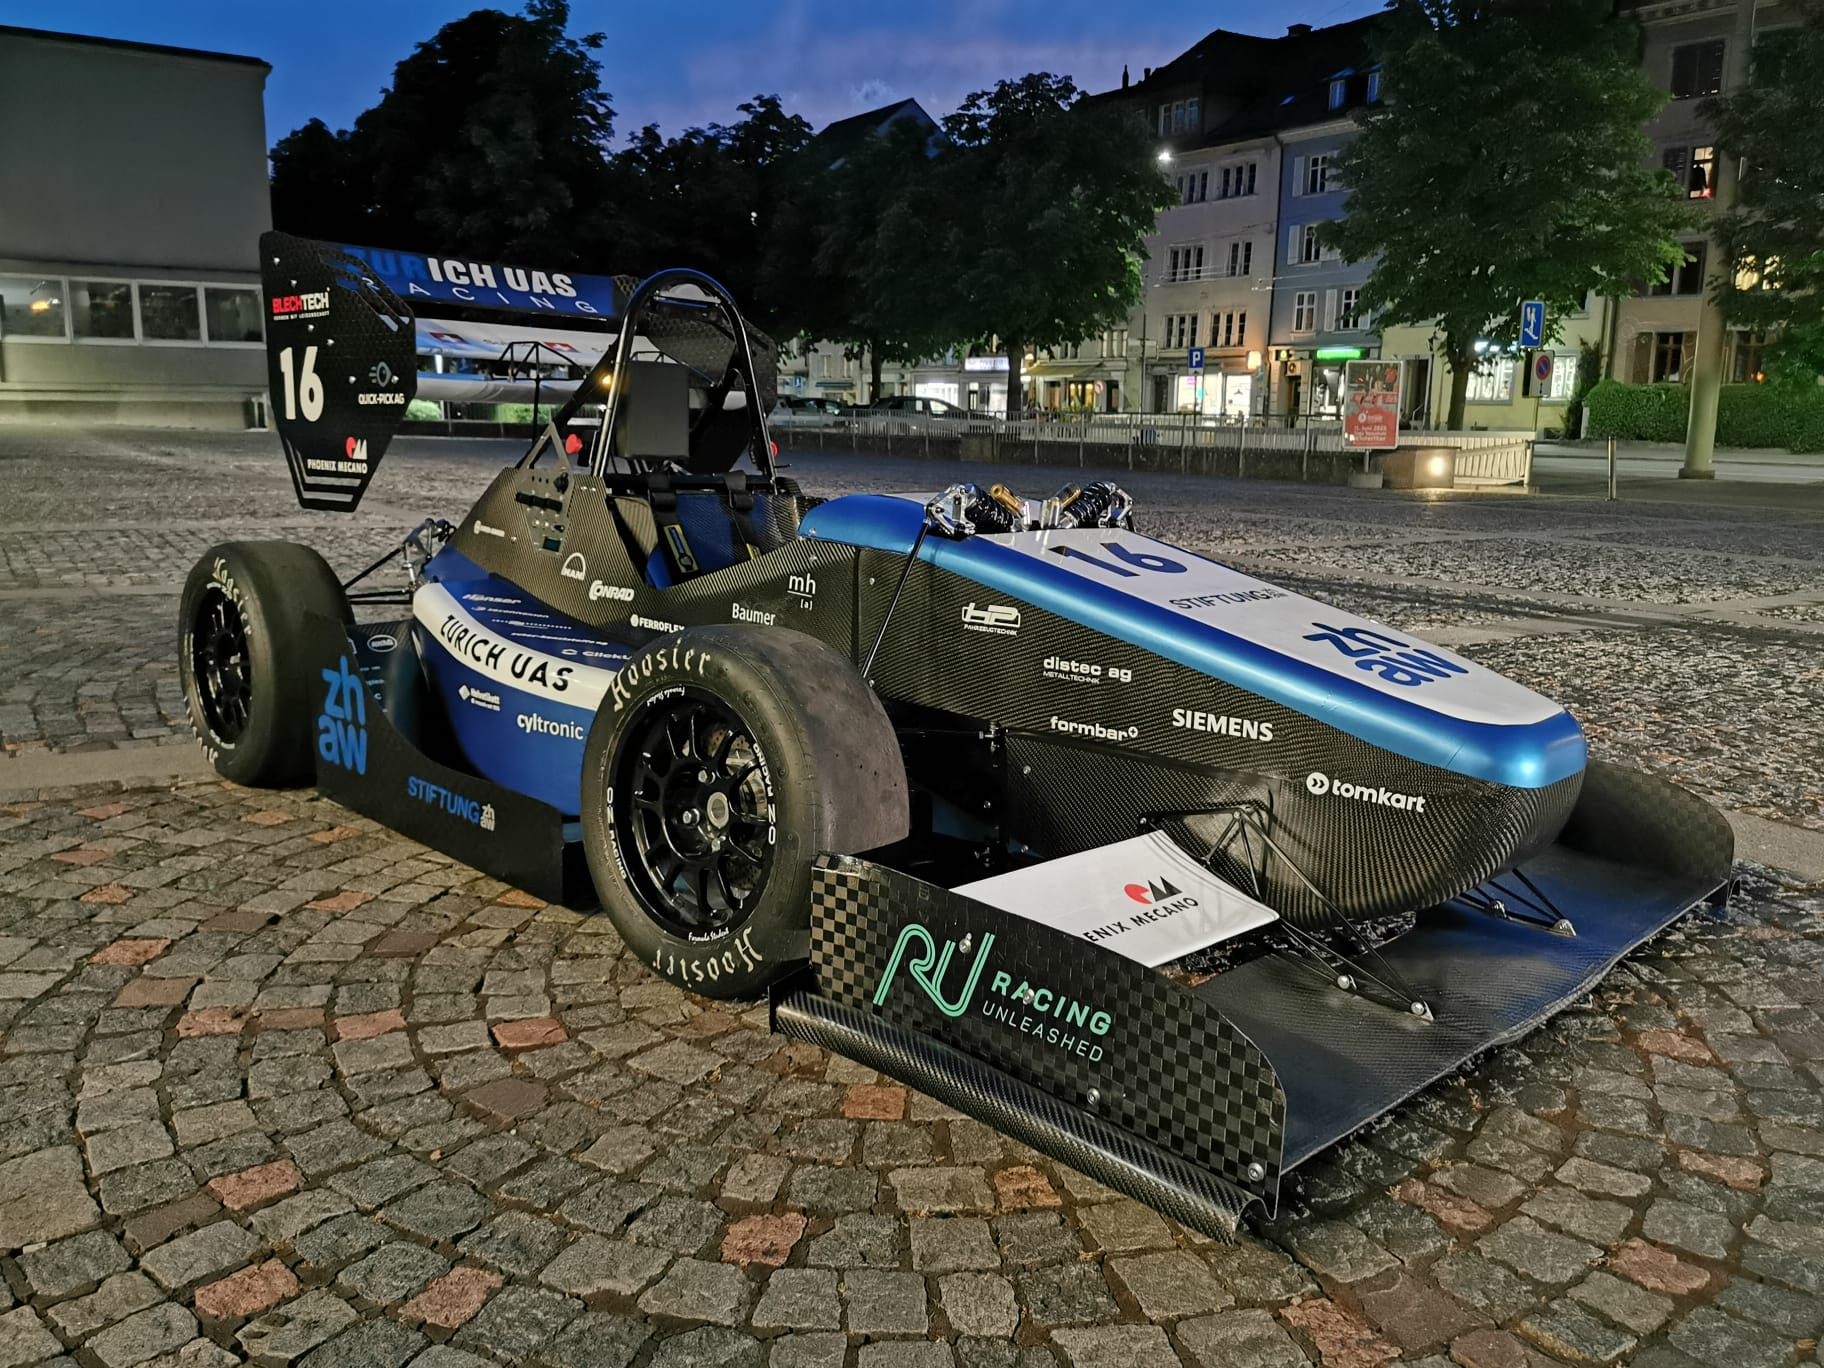
\includegraphics[width=12cm]{ZUR_Racecar_2.jpg}
    \caption{The new second race car of \acrlong{zur}.}
    \label{fig:ZUR Racecar 2}
\end{figure}

As mentioned in section \ref{sec:Optimization Algorithm}, it was decided to use the Minimum Curvature objective for the Optimization Algorithm primarily. Therefore, the algorithm was tested with the Minimum Curvature objective to calculate one, two, three, five and eight laps on a given track, the Fibonacci sequence until eight. Additionally, the Shortest Path objective and the Minimum Curvature objective with iterative call were tested with two laps on a given track. During each run, the total runtime of the algorithm, the estimated lap time with the used objective, and the generated reference points were measured.

\section{Acceleration Track} \label{sec:Results Acceleration Track}
An overview of the track is shown in figure \ref{fig:Results Acceleration Initial}. As mentioned in section \ref{sec:Dynamic Events}, the track is over 75 m in length and tests the car acceleration in a straight line. The track comprises 14 blue cones and 14 yellow cones marking the track limits, 12 orange cones marking the zone where the car should stop, and six big orange cones marking the start and end of the track.
\begin{figure}[H]
    \centering
    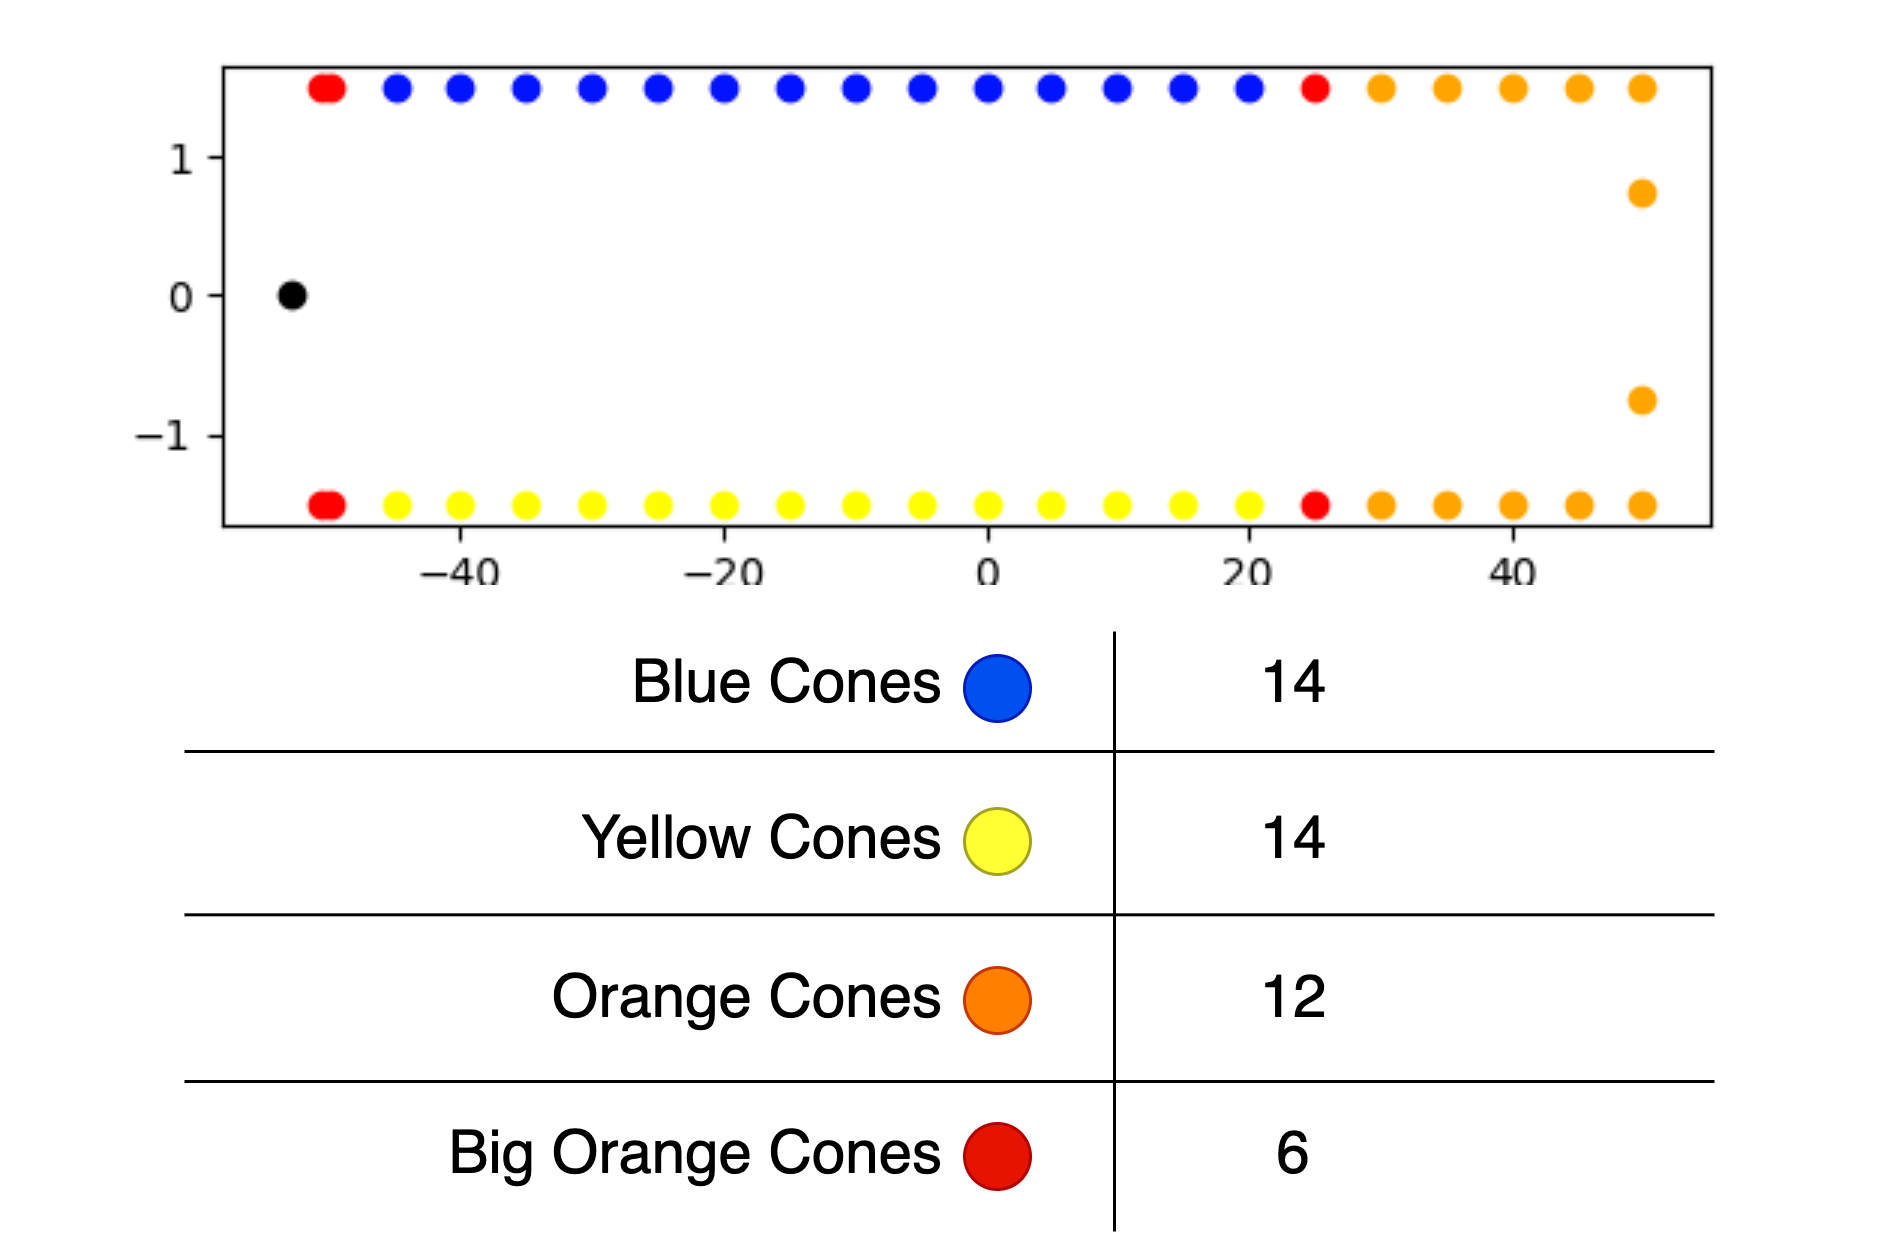
\includegraphics[width=\columnwidth]{Results_Acceleration_Initial.png}
    \caption{Overview of the Acceleration Track.}
    \label{fig:Results Acceleration Initial}
\end{figure}

As Acceleration is a point-to-point race, an optimization after a full lap is not possible in this case.

\textbf{Exploration Algorithm}

During the run with the Acceleration track, the algorithm did 43 cycles with a total computation time of 0.0671 seconds. The average cycle lasted 0.0016 seconds, with the fastest cycle taking under < 0.0000 seconds long and the slowest cycle taking 0.0028 seconds long. The algorithm created 59 reference points during the run. The results are listed in table \ref{tab:Results Acceleration Exploration}.

\begin{table}[H]
    \centering
    \begin{tabular}{|l|l|l|}
        \hline
        \textbf{Result}            & \textbf{Value} \\ \hline
        Minimum Cycle Time         & < 0.0000 s     \\ \hline
        Maximum Cycle Time         & 0.0028 s       \\ \hline
        Average Cycle  Time        & 0.0016 s       \\ \hline
        Total Cycle Time           & 0.0671 s       \\ \hline
        Number of Cycles           & 43             \\ \hline
        Generated Reference Points & 59             \\ \hline
    \end{tabular}
    \caption{Results of the Exploration Algorithm on Acceleration.}
    \label{tab:Results Acceleration Exploration}
\end{table}

Figure \ref{fig:Result Acceleration First Approaches} shows the first approach (a) and the second (b) approach side by side on the acceleration track, which was described in section \ref{sec:Dynamic Events}. The second approach calculated the middle points between the grouped four points used for the triangulation. In addition to the added points, a line was drawn to smoothen the track. Since the plot on (a) and (b) do not plot the start and the end cones (orange cones), they were just used as a basis for the final, more usable algorithm implementation seen in figure \ref{fig:Result Acceleration Final}.
\begin{figure}[H]
    \centering
    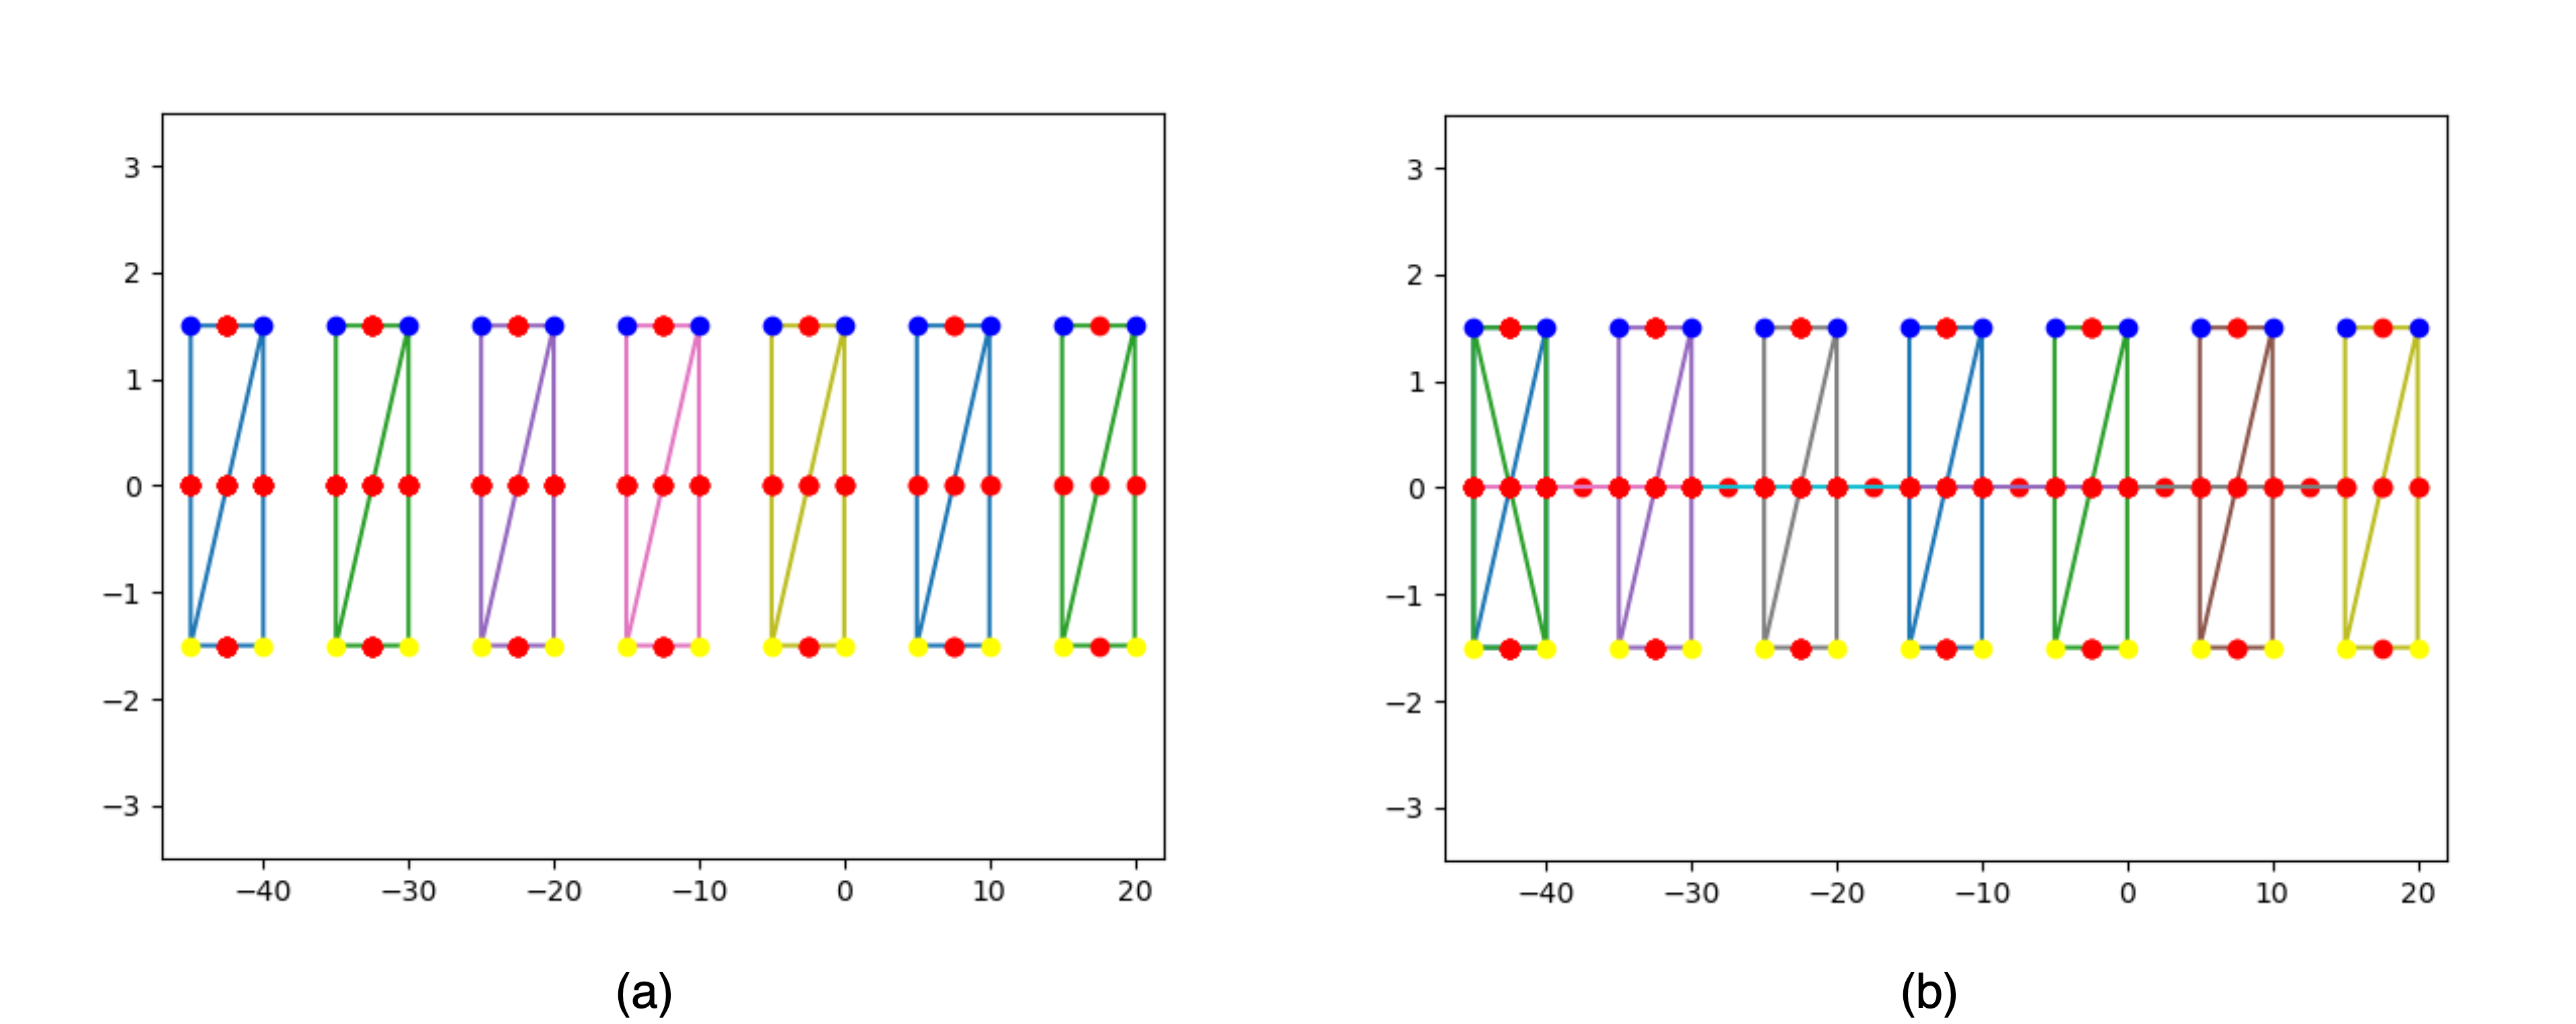
\includegraphics[width=\columnwidth]{Result_Acceleration_First_Approaches.png}
    \caption{Image (a) shows the first approach on the acceleration track, while image (b) shows the second while drawing a middle line.}
    \label{fig:Result Acceleration First Approaches}
\end{figure}
\begin{figure}[H]
    \centering
    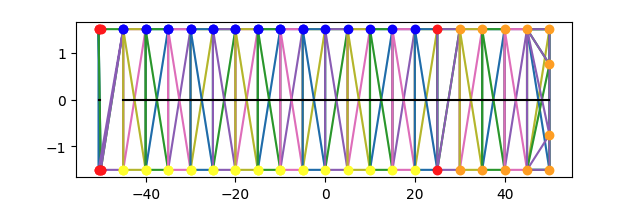
\includegraphics[width=\columnwidth]{Result_Acceleration_final.png}
    \caption{The image shows the final approach on the Acceleration track.}
    \label{fig:Result Acceleration Final}
\end{figure}

\section{Skidpad Track} \label{sec:Results Skidpad Track}
An overview of the track is shown in figure \ref{fig:Results Skidpad Initial}. As mentioned in section \ref{sec:Dynamic Events}, the track consists of two pairs of concentric circles in the shape of an eight and will test the lateral grip of the car. The track comprises 30 blue cones and 30 yellow cones marking the track limits, 20 orange cones marking the start and stopping zones, and four big orange cones marking the beginnings and ends of the concentric circles.
\begin{figure}[H]
    \centering
    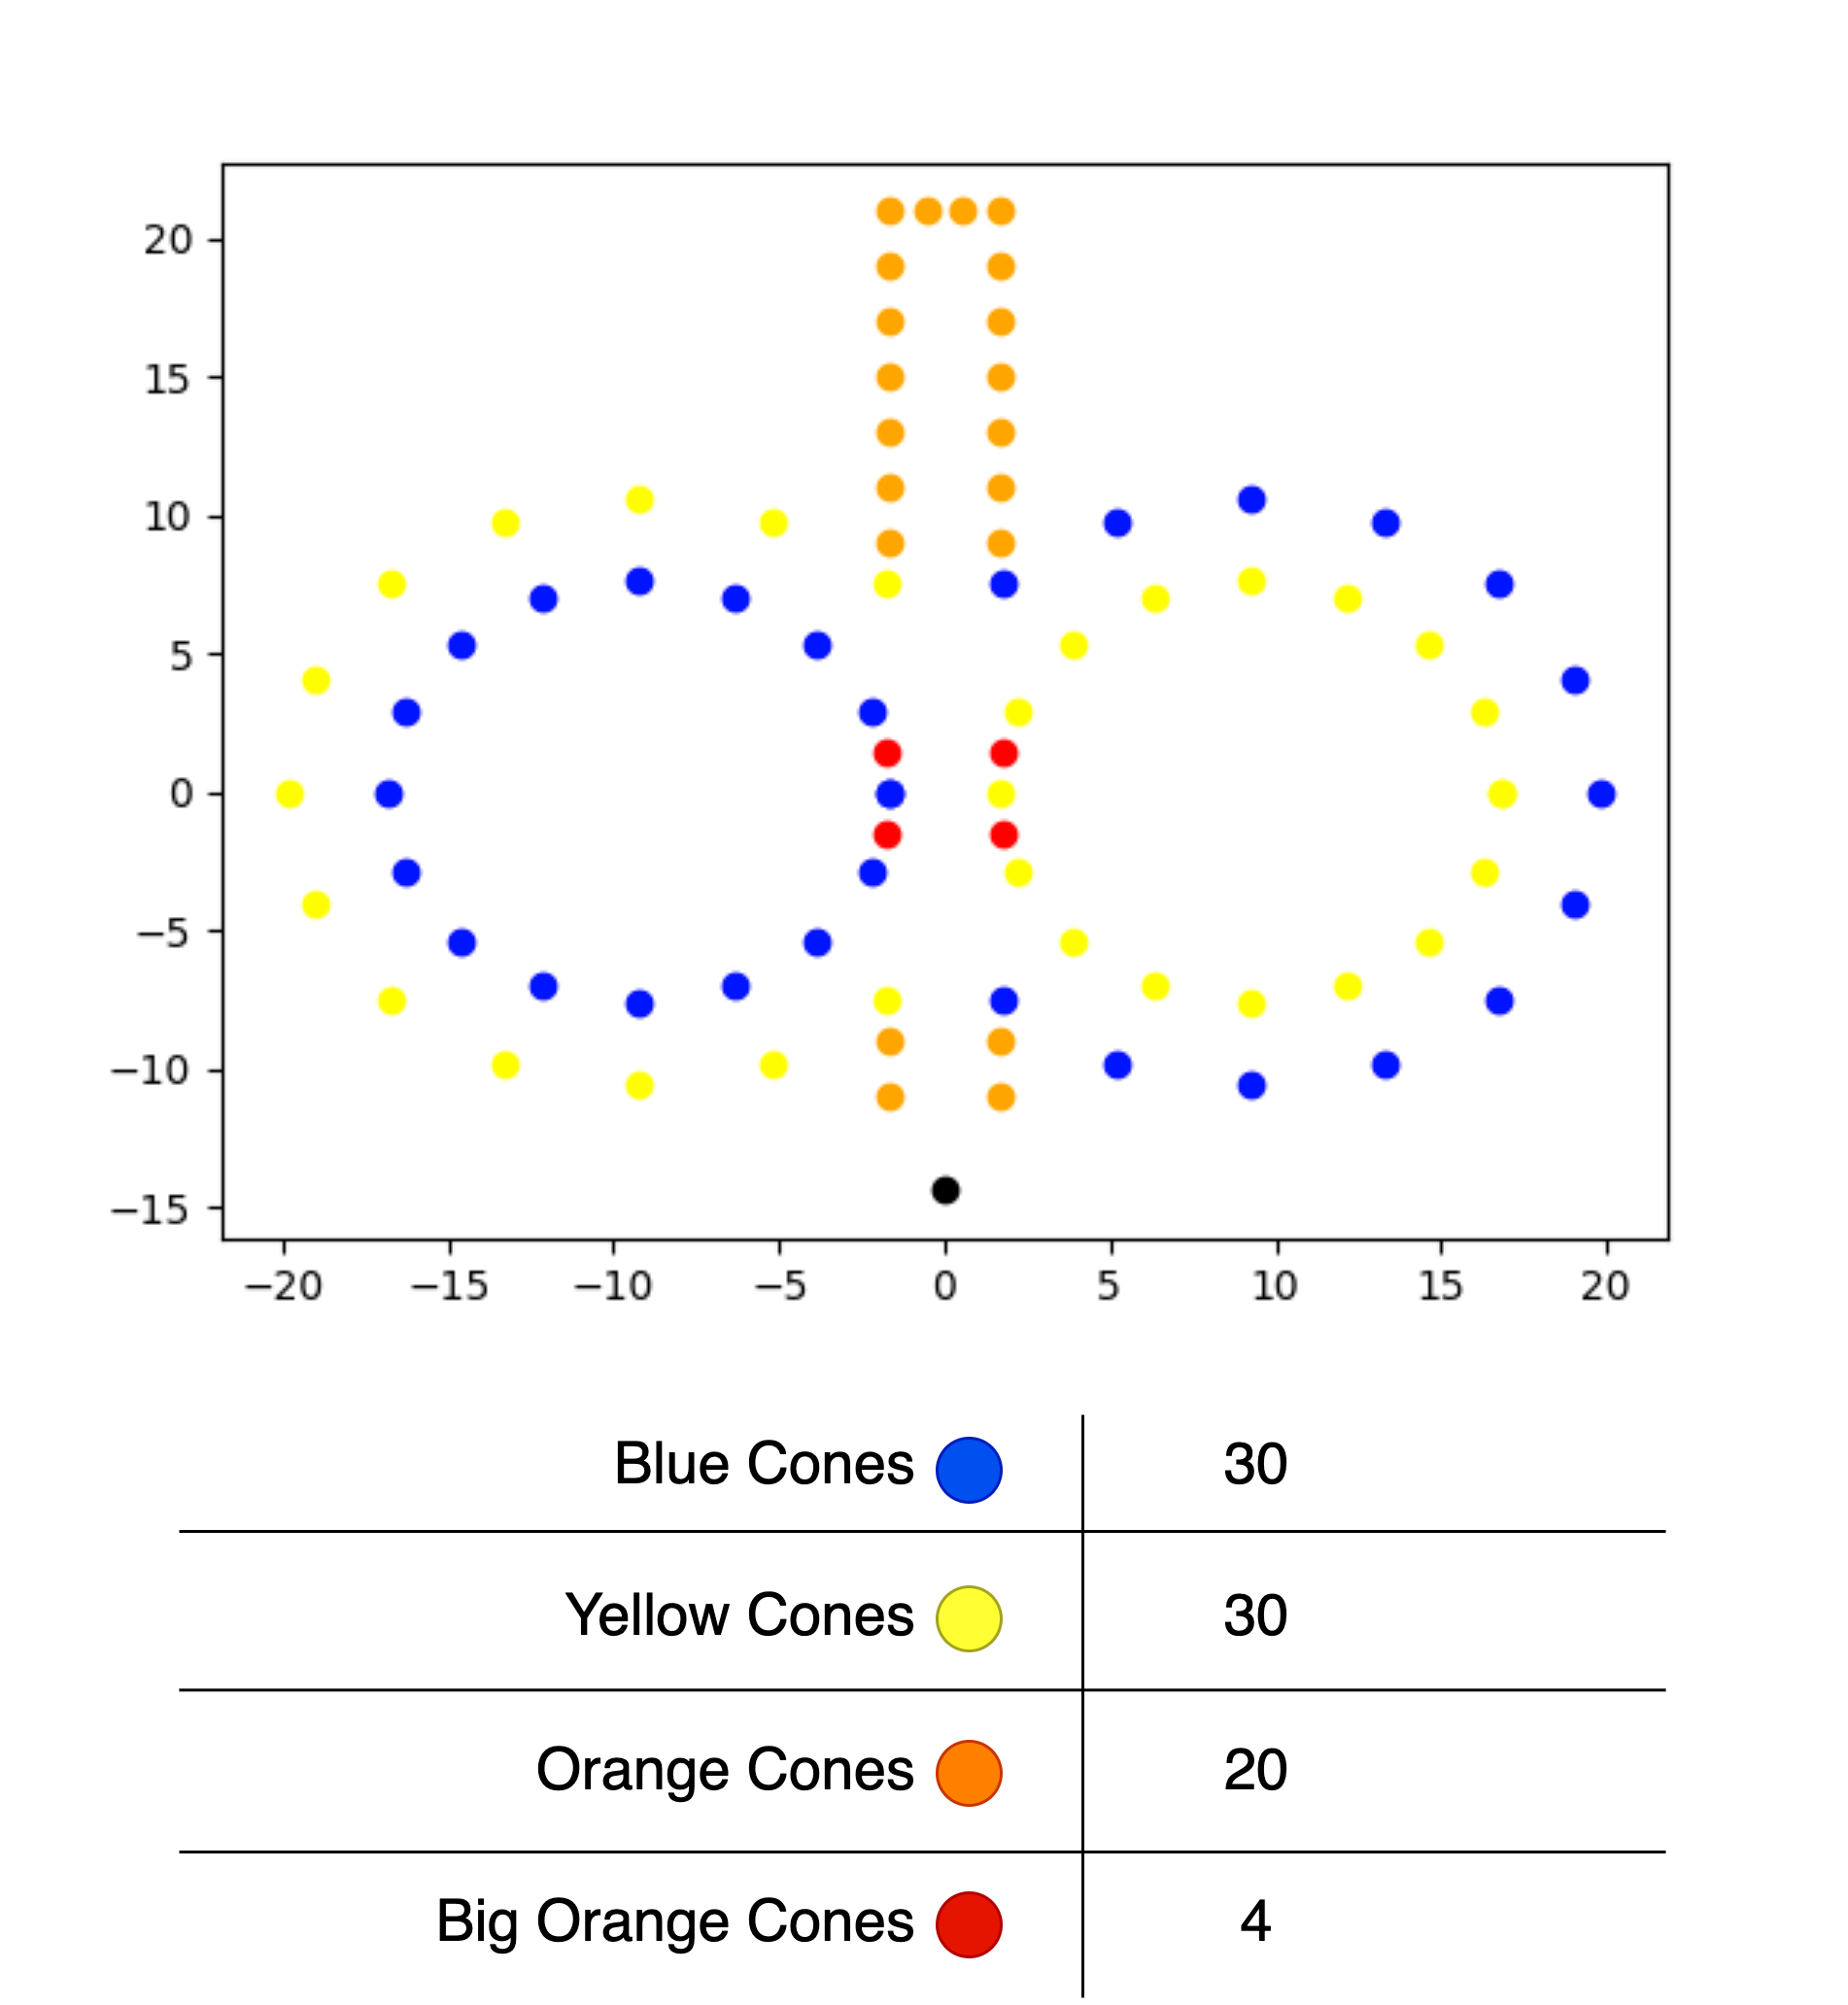
\includegraphics[width=\columnwidth]{Results_Skidpad_Initial.png}
    \caption{Overview of the Skidpad Track.}
    \label{fig:Results Skidpad Initial}
\end{figure}

As Skidpad is a point-to-point race, an optimization after a full lap is not possible in this case.

\textbf{Exploration Algorithm}

During the run with the Skidpad track, the algorithm did 103 cycles with a total computation time of 0.2169 seconds. The average cycle lasted 0.0021 seconds, with the fastest cycle taking 0.0001 seconds long and the slowest cycle taking 0.0051 seconds long. The algorithm created 859 reference points during the run. The results are listed in table \ref{tab:Results Skidpad Exploration}.

\begin{table}[H]
    \centering
    \begin{tabular}{|l|l|l|}
        \hline
        \textbf{Result}            & \textbf{Value} \\ \hline
        Minimum Cycle Time         & 0.0001 s       \\ \hline
        Maximum Cycle Time         & 0.0051 s       \\ \hline
        Average Cycle  Time        & 0.0021 s       \\ \hline
        Total Cycle Time           & 0.2169 s       \\ \hline
        Number of Cycles           & 103            \\ \hline
        Generated Reference Points & 859            \\ \hline
    \end{tabular}
    \caption{Results of the Exploration Algorithm on Skidpad.}
    \label{tab:Results Skidpad Exploration}
\end{table}

Figure \ref{fig:Result Skidpad Final} shows the application of the algorithm on the Skidpad track.
\begin{figure}[H]
    \centering
    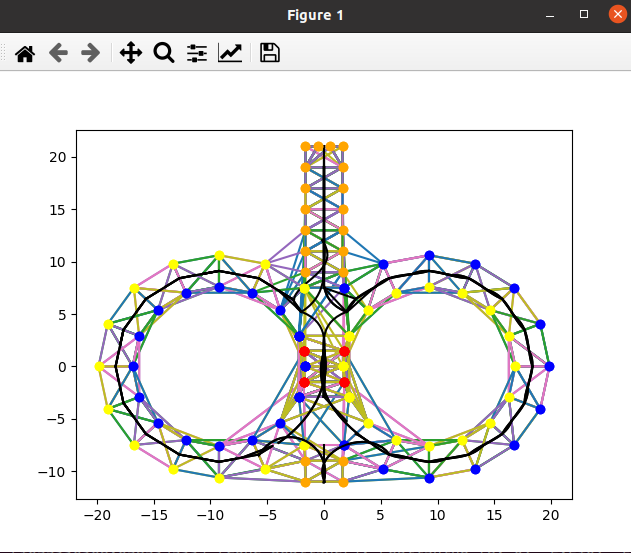
\includegraphics[width=\columnwidth]{Result_Skidpad_final.png}
    \caption{The calculation of the middle line on the Skidpad track.}
    \label{fig:Result Skidpad Final}
\end{figure}

\section{Small Track} \label{sec:Results Small Track}
An overview of the track is shown in figure \ref{fig:Results Small Track Initial}. The track was created by the \acrshort{eufs} team and is called ``Small Track''. \cite{eufs_sim_gitlab} The track helped to get an understanding of how the algorithm works on corners with fewer cones on the inner side than on the outer side. The track consists of 37 blue cones and 30 yellow cones for the track limits, and 4 big orange cones for the start respectively the end of the track.
\begin{figure}[H]
    \centering
    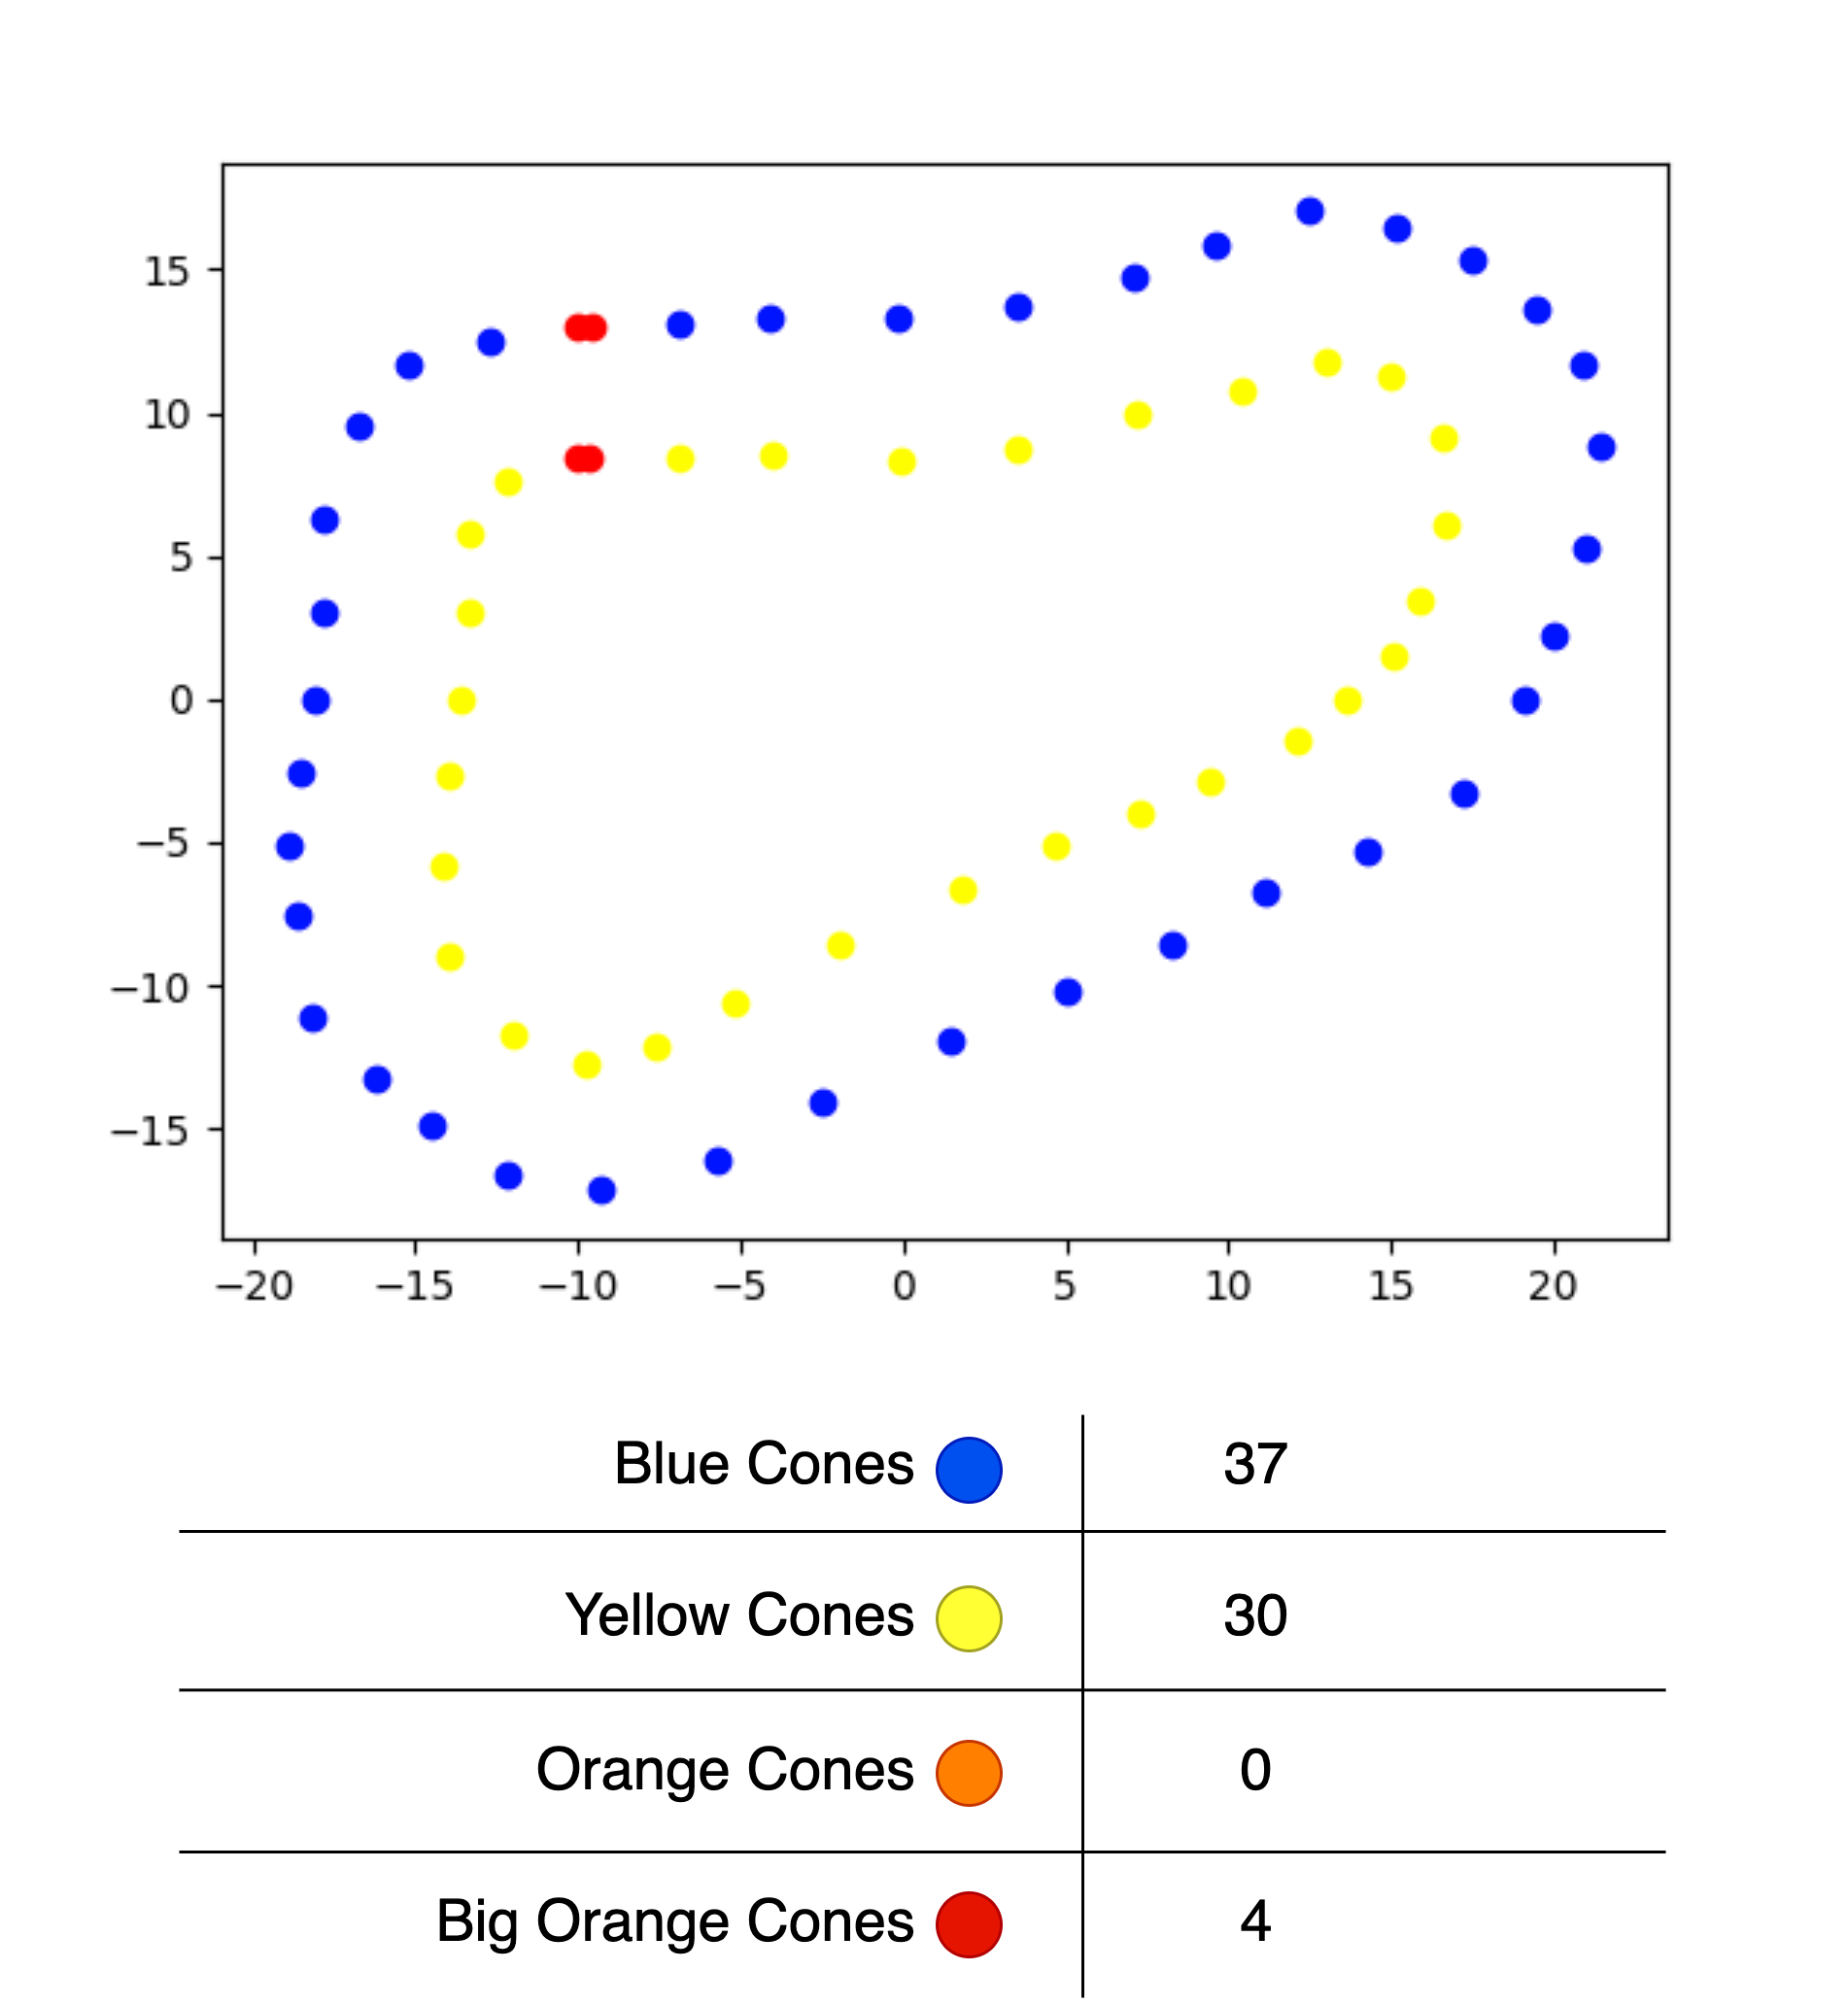
\includegraphics[width=\columnwidth]{Results_Small_Track_Initial.png}
    \caption{Overview of the Small Track.}
    \label{fig:Results Small Track Initial}
\end{figure}

\textbf{Exploration Algorithm}

During the run with the ``Small Track'' track, the algorithm did 71 cycles with a total computation time of 0.1974 seconds. The average cycle lasted 0.0028 seconds, with the fastest cycle taking under < 0.0000 seconds long and the slowest cycle taking 0.0066 seconds long. The algorithm created 865 reference points during the run. The results are listed in table \ref{tab:Results Small Track Exploration}.

\begin{table}[H]
    \centering
    \begin{tabular}{|l|l|l|}
        \hline
        \textbf{Result}            & \textbf{Value} \\ \hline
        Minimum Cycle Time         & < 0.0000 s     \\ \hline
        Maximum Cycle Time         & 0.0066 s       \\ \hline
        Average Cycle  Time        & 0.0028 s       \\ \hline
        Total Cycle Time           & 0.1974 s       \\ \hline
        Number of Cycles           & 71             \\ \hline
        Generated Reference Points & 865            \\ \hline
    \end{tabular}
    \caption{Results of the Exploration Algorithm on Small Track.}
    \label{tab:Results Small Track Exploration}
\end{table}

Figure \ref{fig:Result Small Track First Approaches} shows a progression of the improvements of the first implementation of the algorithm (a) to the second improved version (b) and the final version of the algorithm in figure \ref{fig:Result Small Track Final}. Again for the first and the second approach, the implementation of publishing the start and end cones (orange cones) was not made already.
\begin{figure}[H]
    \centering
    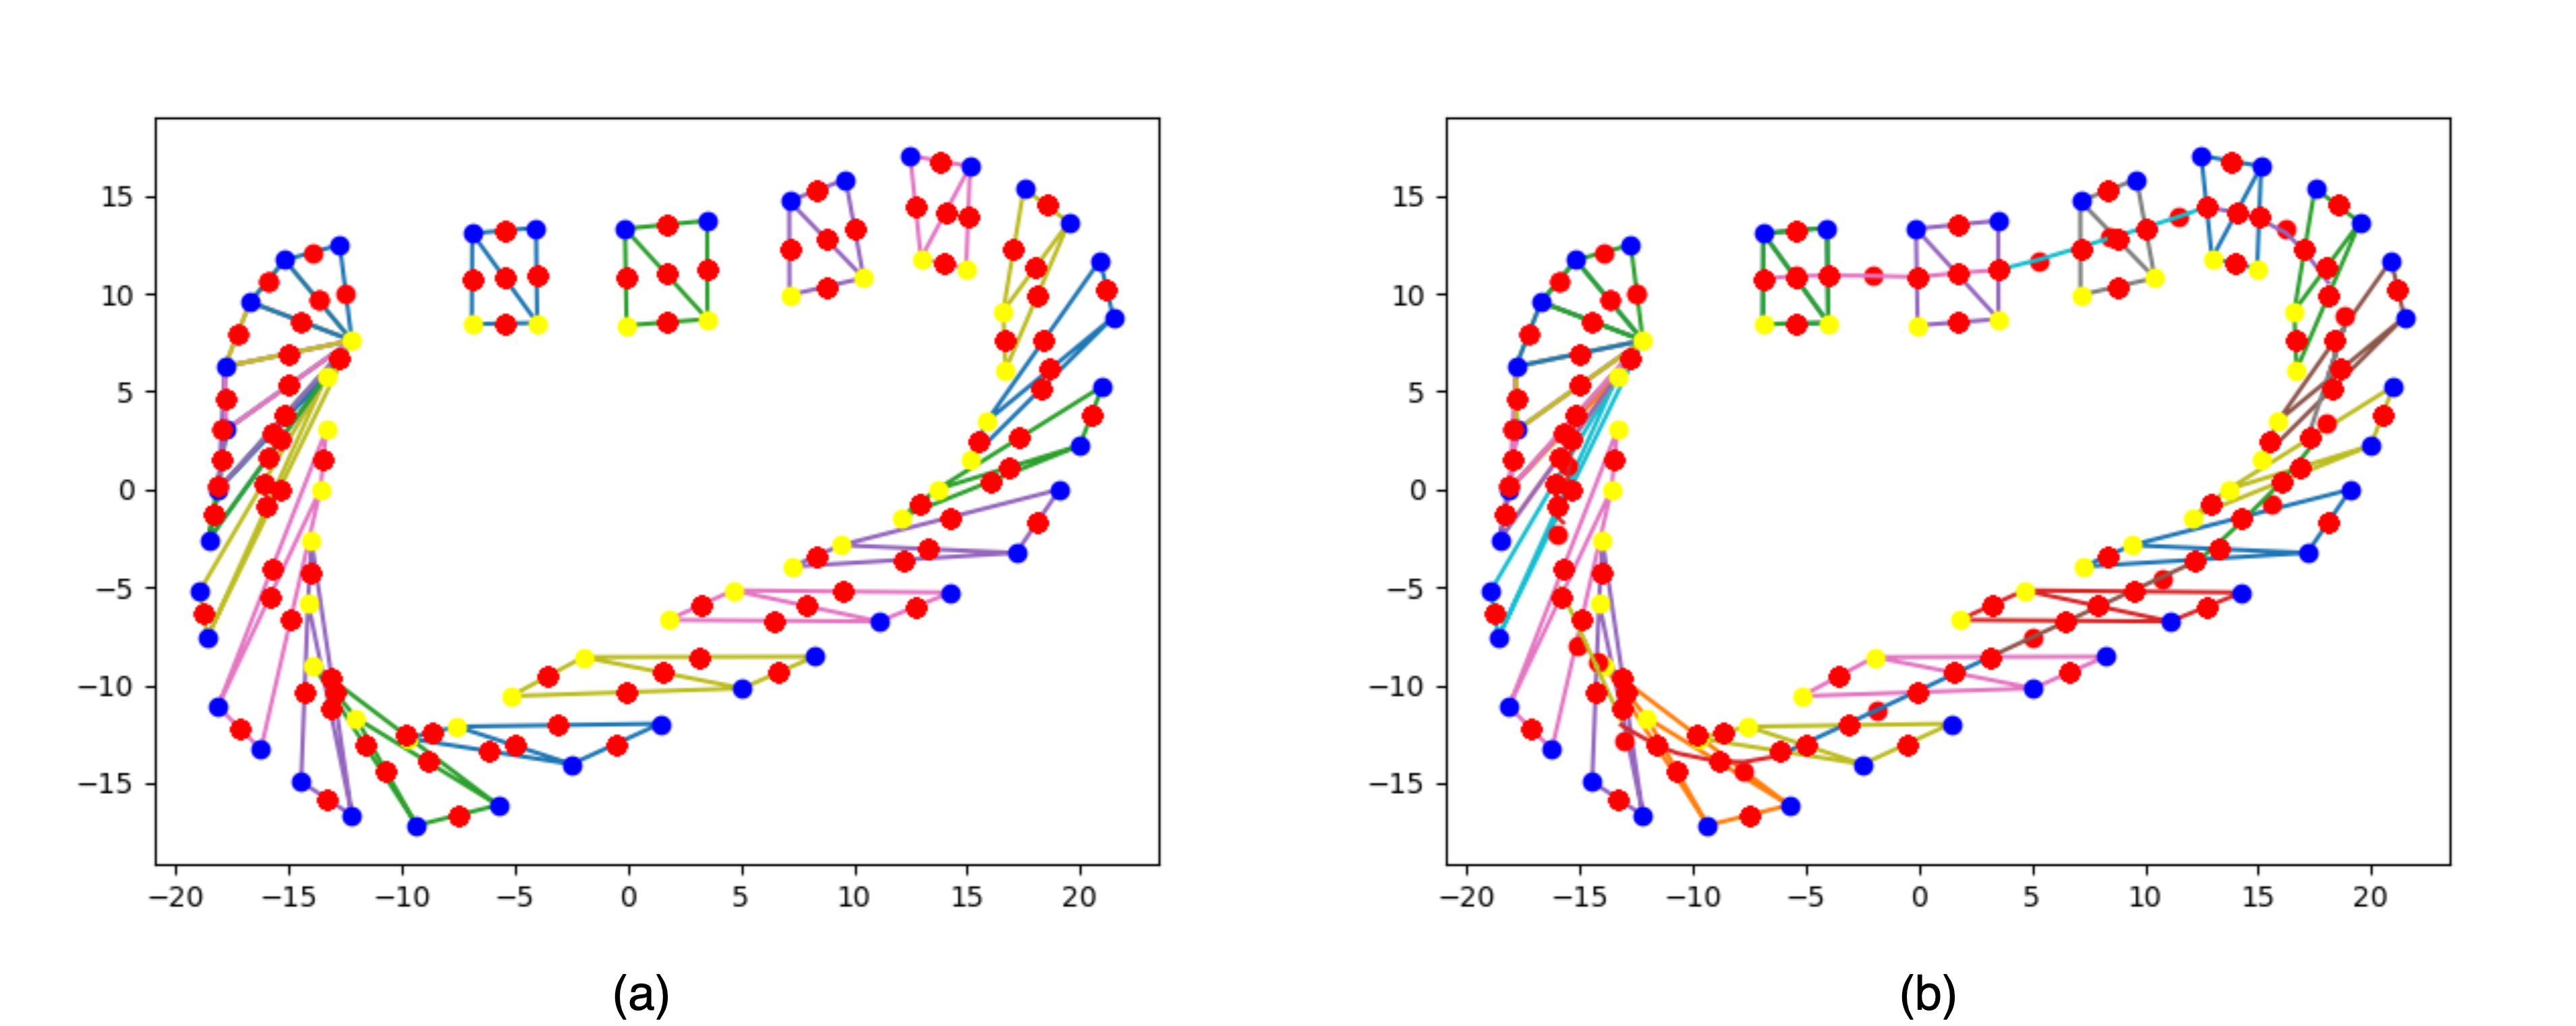
\includegraphics[width=\columnwidth]{Result_SmallTrack_First_Approaches.png}
    \caption{The progression of the improvements of the first implementation (a) to the second implementation (b) is shown.}
    \label{fig:Result Small Track First Approaches}
\end{figure}
\begin{figure}[H]
    \centering
    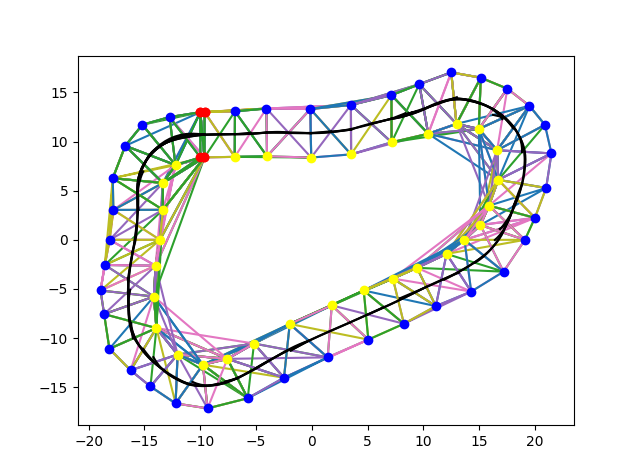
\includegraphics[width=\columnwidth]{Result_SmallTrack_final.png}
    \caption{The image shows the final approach on the Small Track.}
    \label{fig:Result Small Track Final}
\end{figure}

\textbf{Optimization Algorithm}

A comparison of the different objectives on the Small Track is given in table \ref{tab:Results Small Track Optimization Objectives}. Two laps on the given track were calculated for each objective: Shortest Path, Minimum Curvature and Minimum Curvature with iterative call. The result with the Shortest Path objective is seen in figure \ref{fig:Results Small Track Laps 2 Shortest Path}, the result with the Minimum Curvature objective is seen in figure \ref{fig:Results Small Track Laps 2 Minimum Curvature}, and the result with the Minimum Curvature objective with an iterative call is seen in figure \ref{fig:Results Small Track Laps 2 Minimum Curvature IQP}.

\begin{table}[H]
    \centering
    \begin{tabular}{|l|l|l|l|}
        \hline
        \textbf{Objective}    & \textbf{Runtime} & \textbf{Estimated Lap Time} & \textbf{Generated Reference Points} \\ \hline
        Shortest Path         & 0.07 s           & 20.60 s                     & 99 Reference Points                 \\ \hline
        Minimum Curvature     & 0.08 s           & 18.48 s                     & 102 Reference Points                \\ \hline
        Minimum Curvature IQP & 0.10 s           & 17.88 s                     & 102 Reference Points                \\ \hline
    \end{tabular}
    \caption{Results of the different Optimization Algorithm objectives on Small Track for two laps.}
    \label{tab:Results Small Track Optimization Objectives}
\end{table}
\begin{figure}[H]
    \centering
    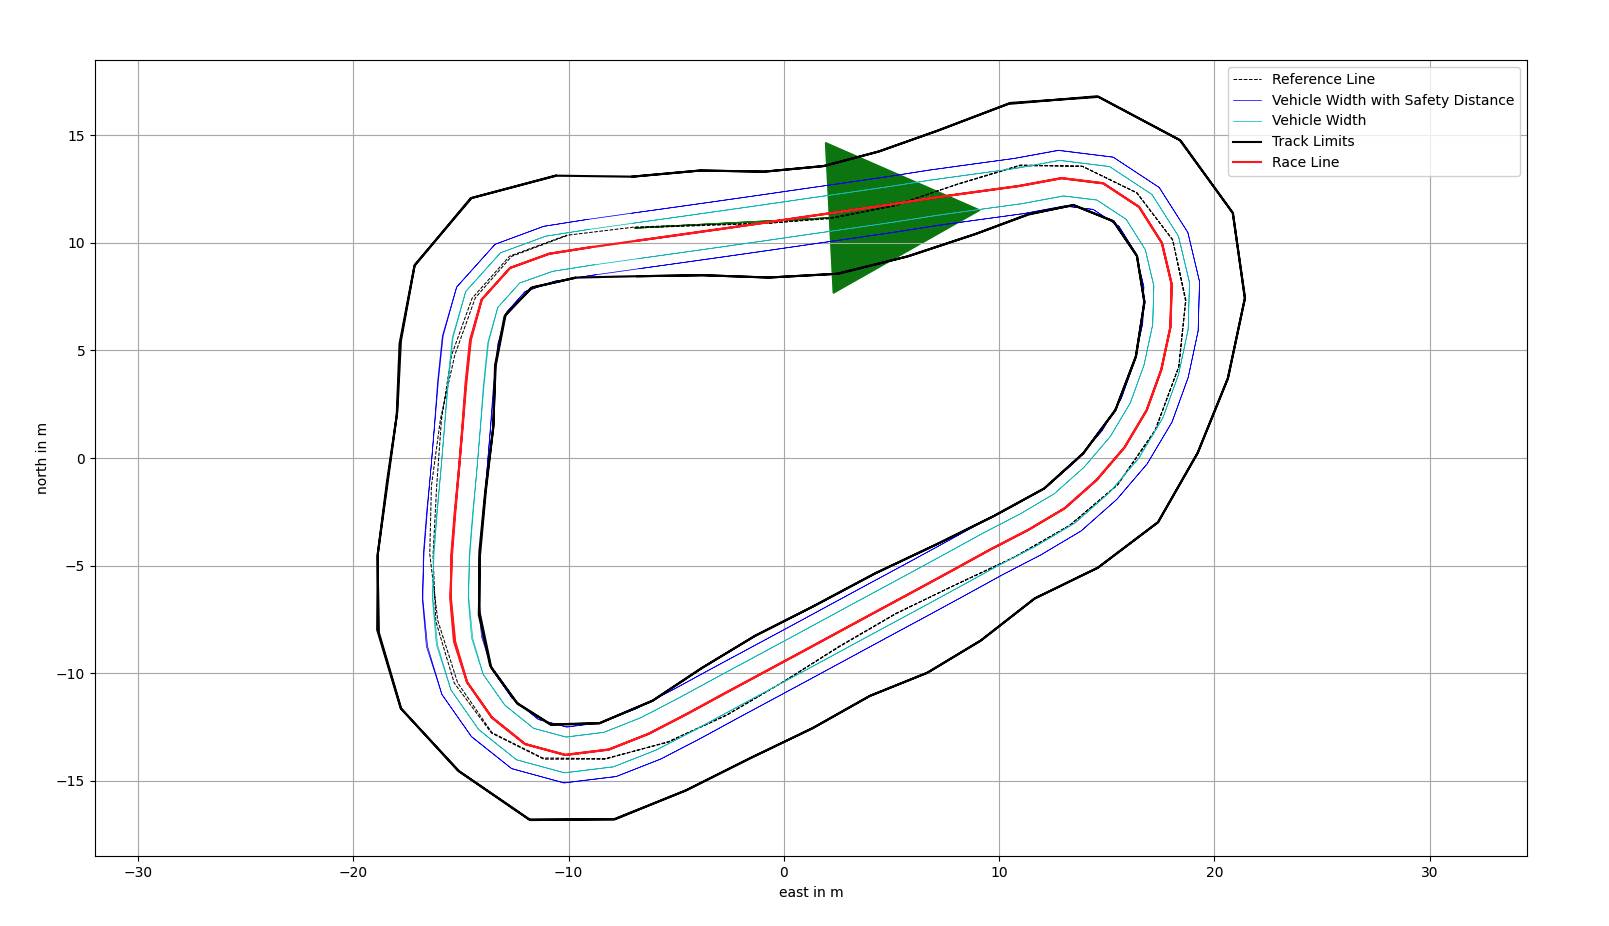
\includegraphics[width=\columnwidth]{Results_Optimization_Small_Track_Laps_2_Shortest_Path.png}
    \caption{Optimization on the Small Track for two laps with the Shortest Path objective.}
    \label{fig:Results Small Track Laps 2 Shortest Path}
\end{figure}
\begin{figure}[H]
    \centering
    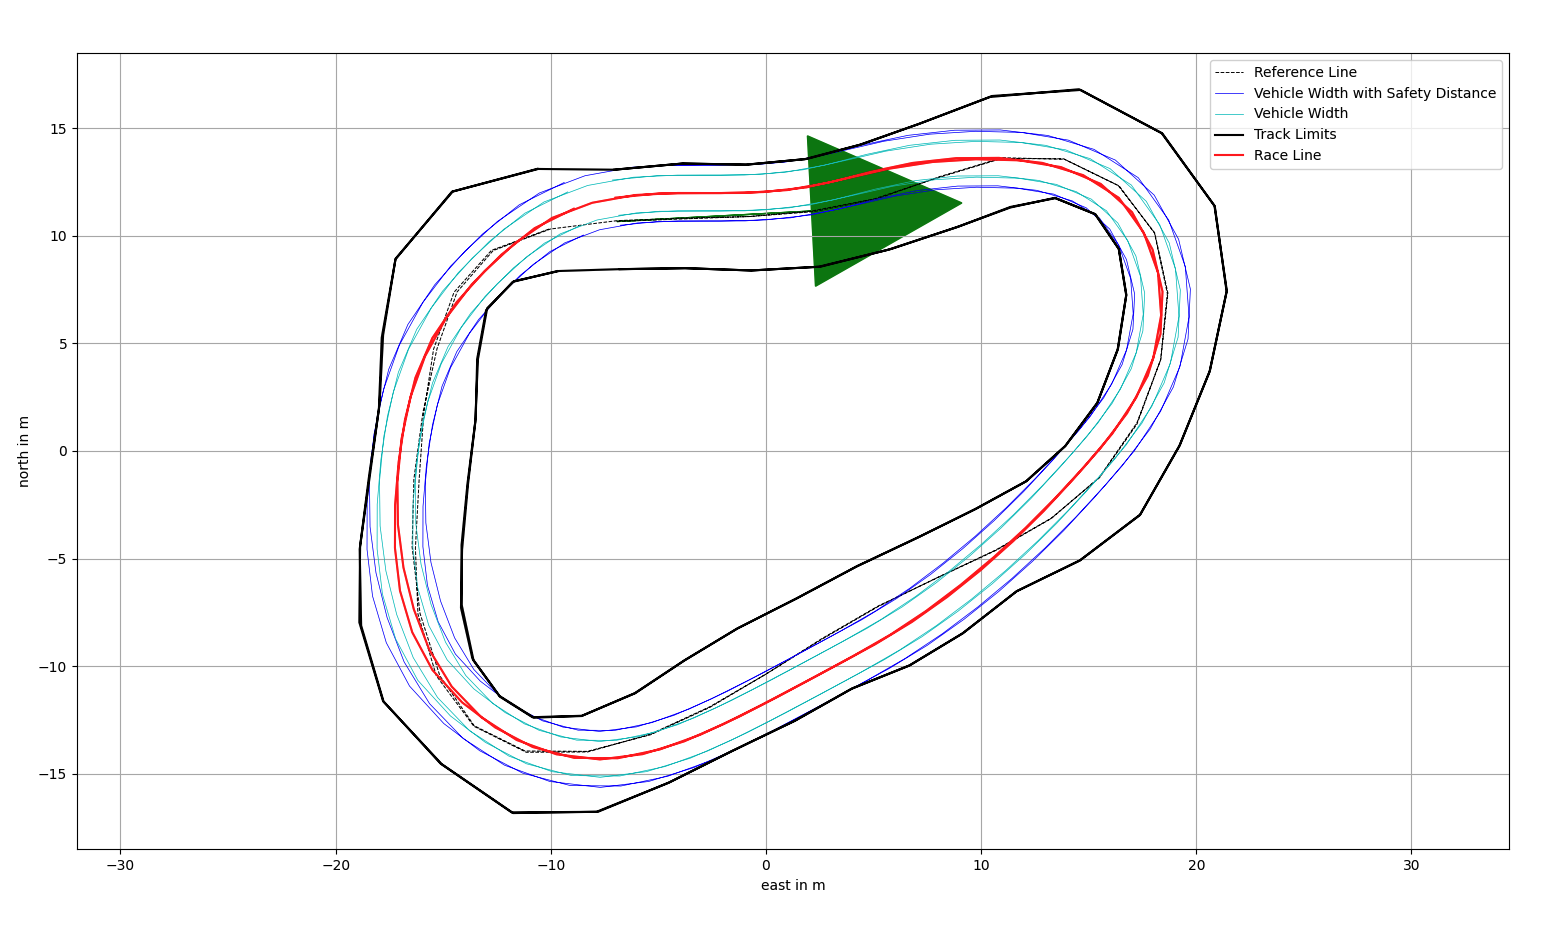
\includegraphics[width=\columnwidth]{Results_Optimization_Small_Track_Laps_2.png}
    \caption{Optimization on the Small Track for two laps with the Minimum Curvature objective.}
    \label{fig:Results Small Track Laps 2 Minimum Curvature}
\end{figure}
\begin{figure}[H]
    \centering
    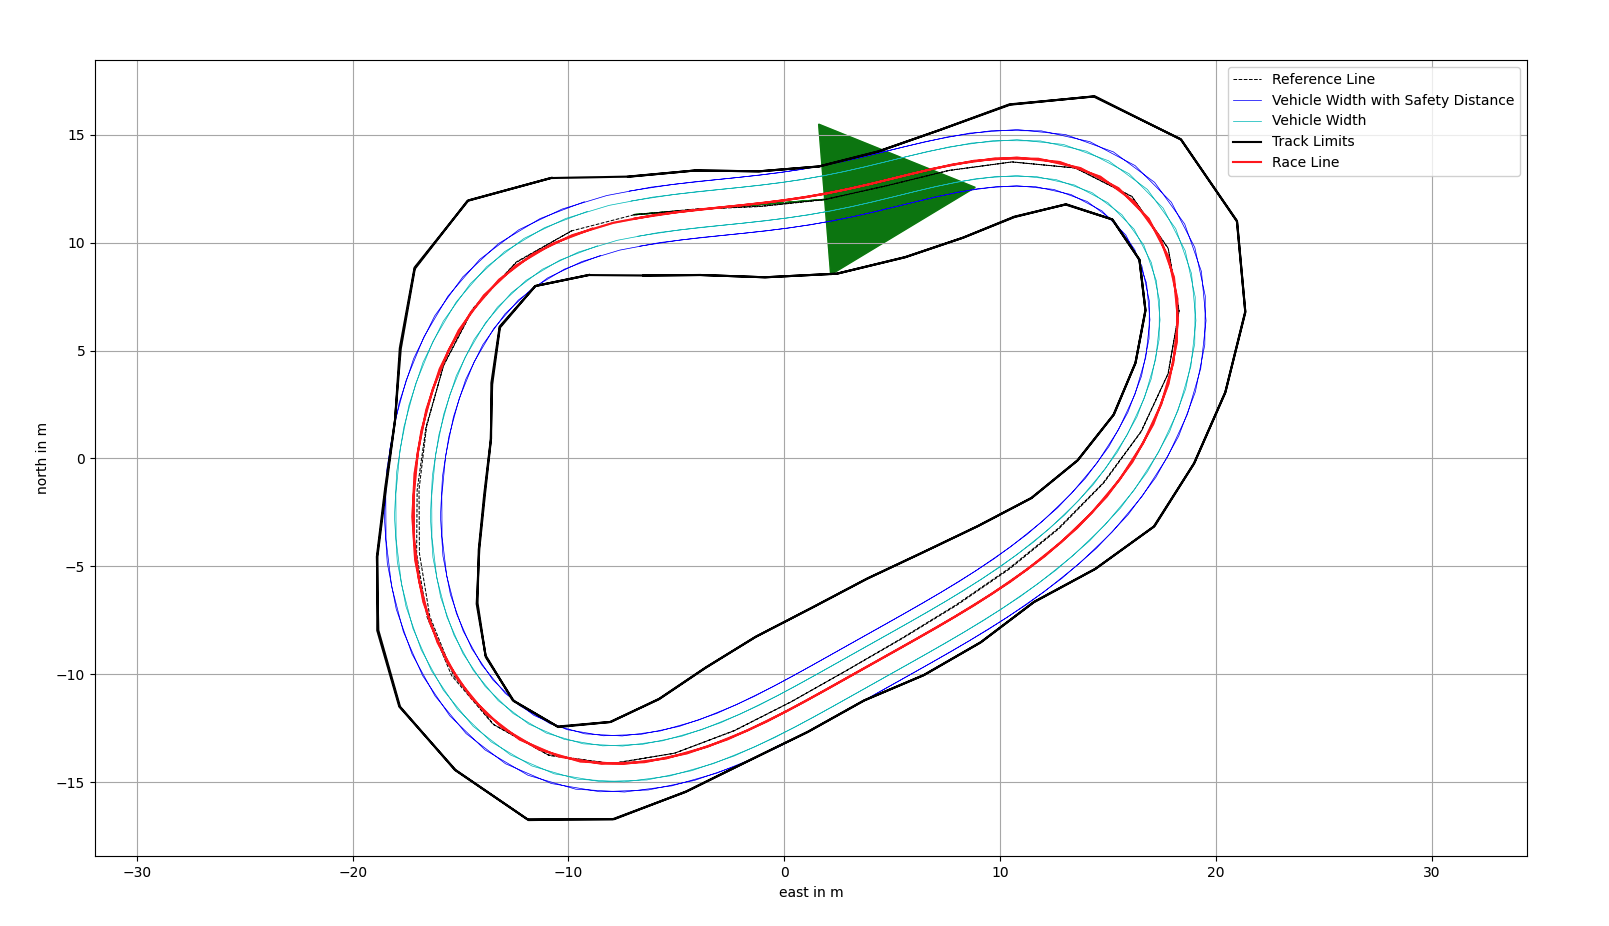
\includegraphics[width=\columnwidth]{Results_Optimization_Small_Track_Laps_2_Mincurv_IQP.png}
    \caption{Optimization on the Small Track for two laps with the Minimum Curvature objective with iterative call.}
    \label{fig:Results Small Track Laps 2 Minimum Curvature IQP}
\end{figure}

The results for the Optimization Algorithm with the Minimum Curvature objective for one lap, two laps, three laps, five laps and eight laps are detailed in table \ref{tab:Results Small Track Optimization Laps 1-8}. The visual comparison of the output between one lap, three laps, five laps and eight laps is shown in figure \ref{fig:Results Small Track Laps 1-8}.

\begin{table}[H]
    \centering
    \begin{tabular}{|l|l|l|l|}
        \hline
        \textbf{Laps} & \textbf{Runtime} & \textbf{Estimated Lap Time} & \textbf{Generated Reference Points} \\ \hline
        1             & 0.04 s           & 9.17 s                      & 52 Reference Points                 \\ \hline
        2             & 0.08 s           & 18.48 s                     & 102 Reference Points                \\ \hline
        3             & 0.12 s           & 28.24 s                     & 152 Reference Points                \\ \hline
        5             & 0.22 s           & 47.39 s                     & 253 Reference Points                \\ \hline
        8             & 0.48 s           & 78.44 s                     & 404 Reference Points                \\ \hline
    \end{tabular}
    \caption{Results of the Optimization Algorithm with the Minimum Curvature objective on Small Track for one to eight laps.}
    \label{tab:Results Small Track Optimization Laps 1-8}
\end{table}
\begin{figure}[H]
    \centering
    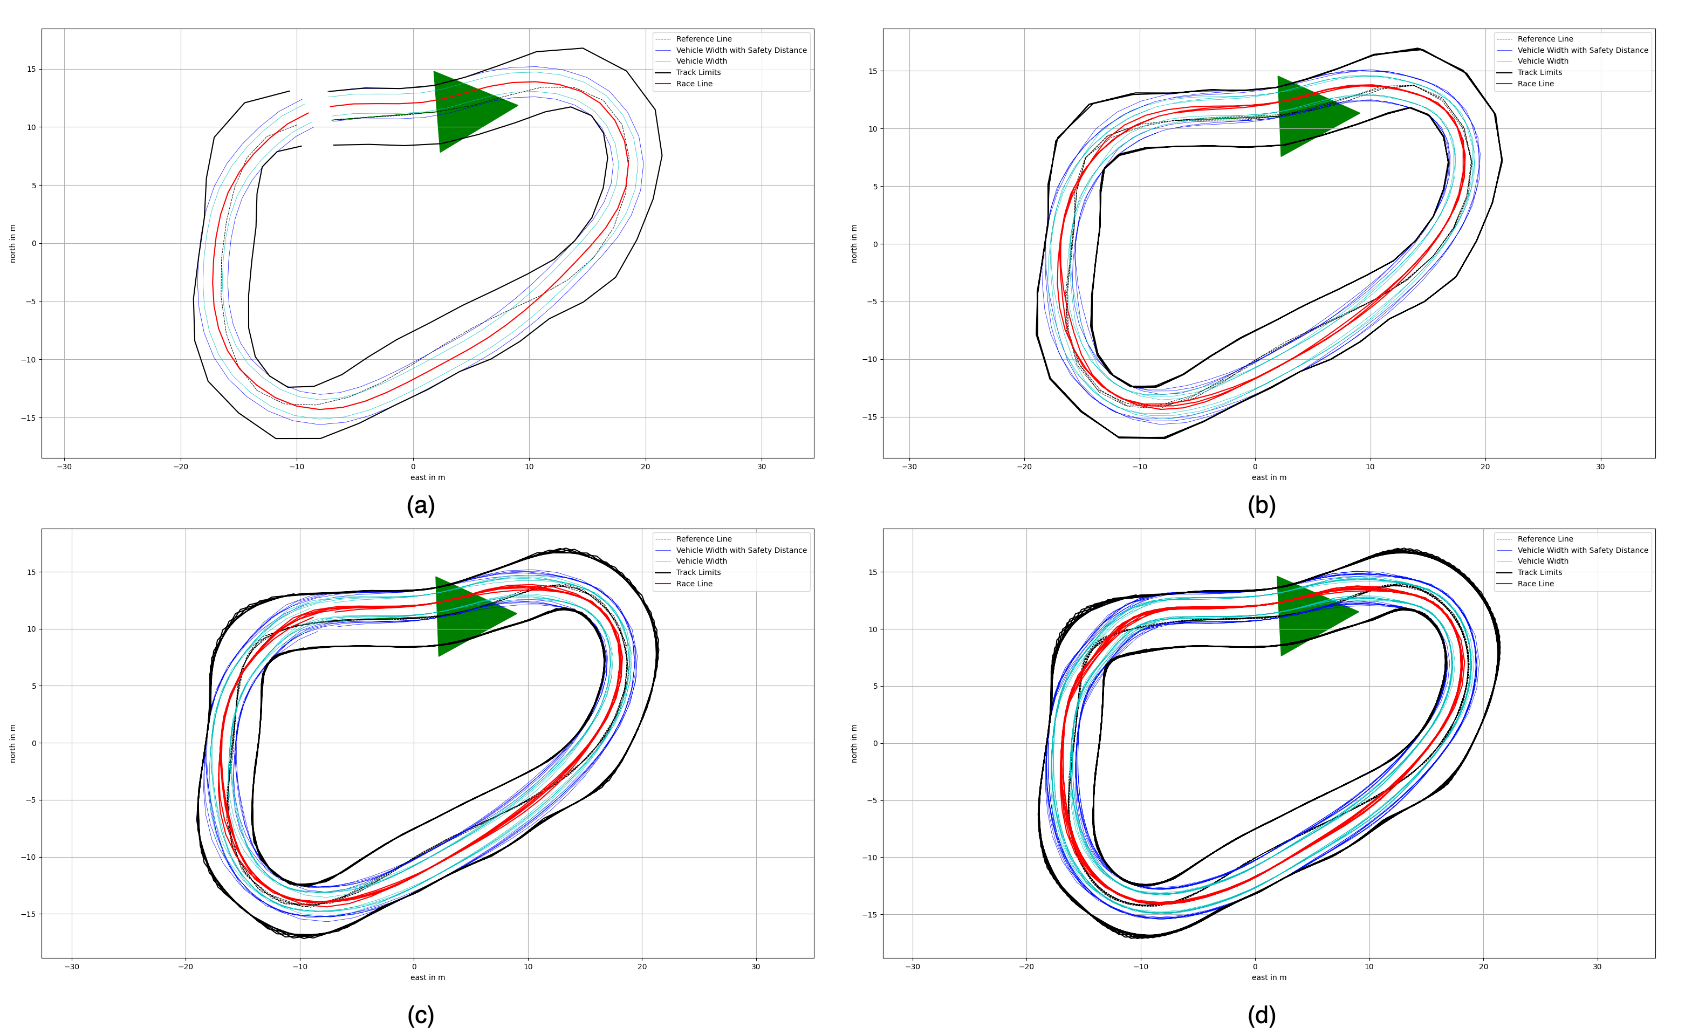
\includegraphics[width=\columnwidth]{Results_Optimization_Small_Track_Laps_1-8.png}
    \caption{Optimization on the Small Track with the Minimum Curvature objective for one lap (a), three laps (b), five laps (c), and eight laps (d).}
    \label{fig:Results Small Track Laps 1-8}
\end{figure}

Additionally, the following outputs of the Optimization Algorithm with the Minimum Curvature objective for two laps on the Small Track are shown: The Velocity and Acceleration Profile in figure \ref{fig:Results Small Track Laps 2 VelAcc Profile}, the Curvature Profile in figure \ref{fig:Results Small Track Laps 2 Curv Profile}, the 3D Velocity Profile in figure \ref{fig:Results Small Track Laps 2 3D Vel Profile}, and the Spline Normals in figure \ref{fig:Results Small Track Laps 2 Spline Normals}.
\begin{figure}[H]
    \centering
    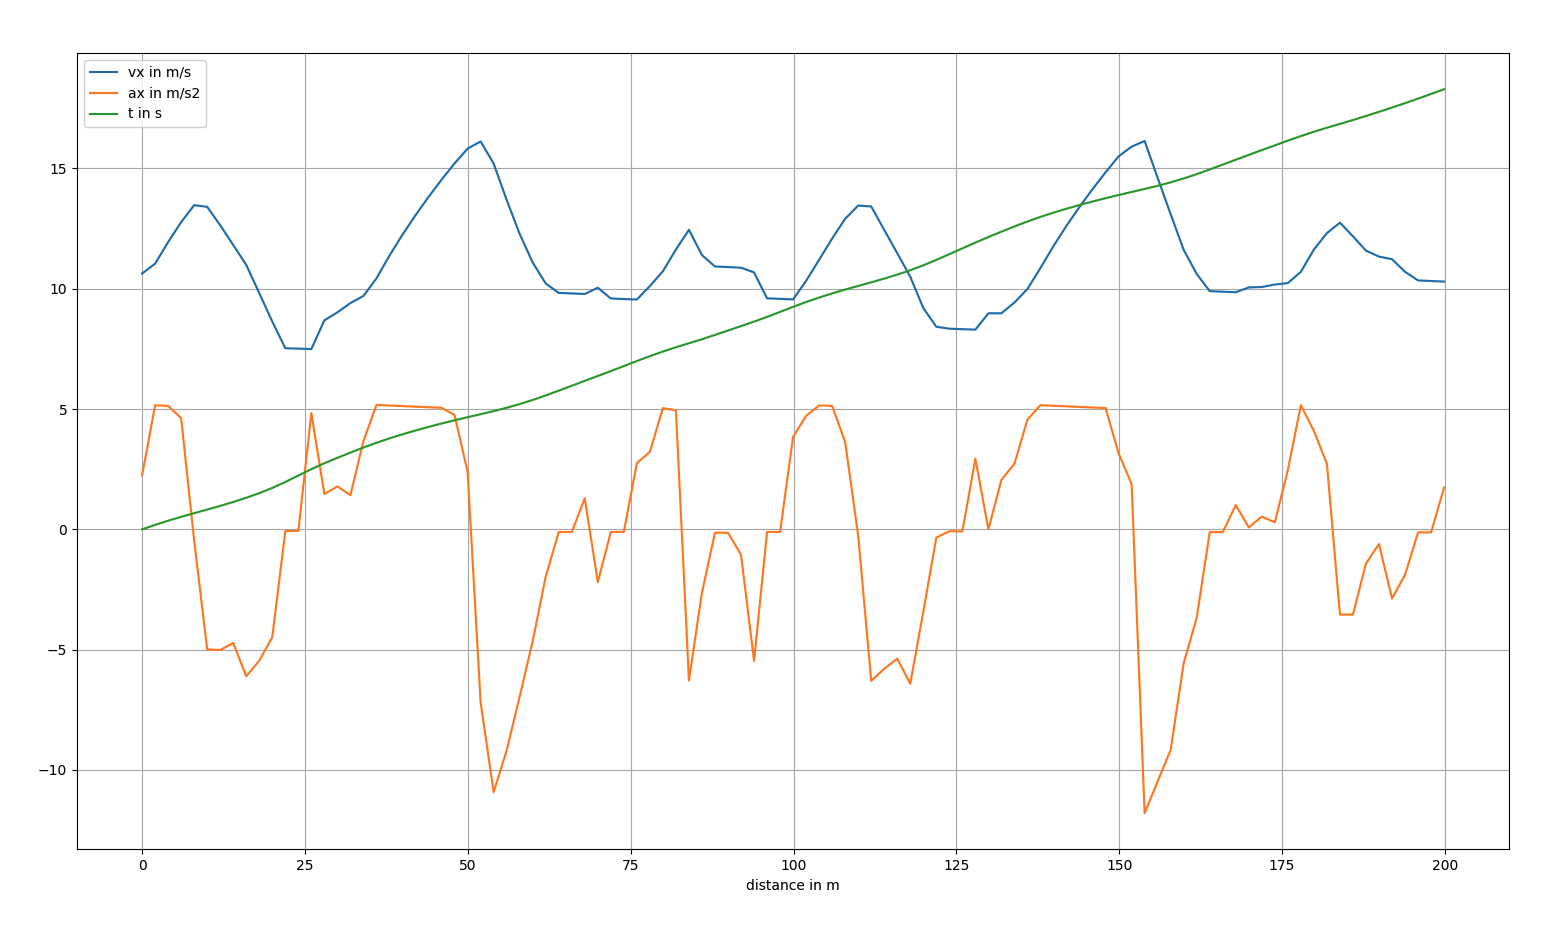
\includegraphics[width=\columnwidth]{Results_Optimization_Small_Track_Laps_2_VelAcc_Profile.png}
    \caption{The Velocity and Acceleration Profile on Small Track for two laps.}
    \label{fig:Results Small Track Laps 2 VelAcc Profile}
\end{figure}
\begin{figure}[H]
    \centering
    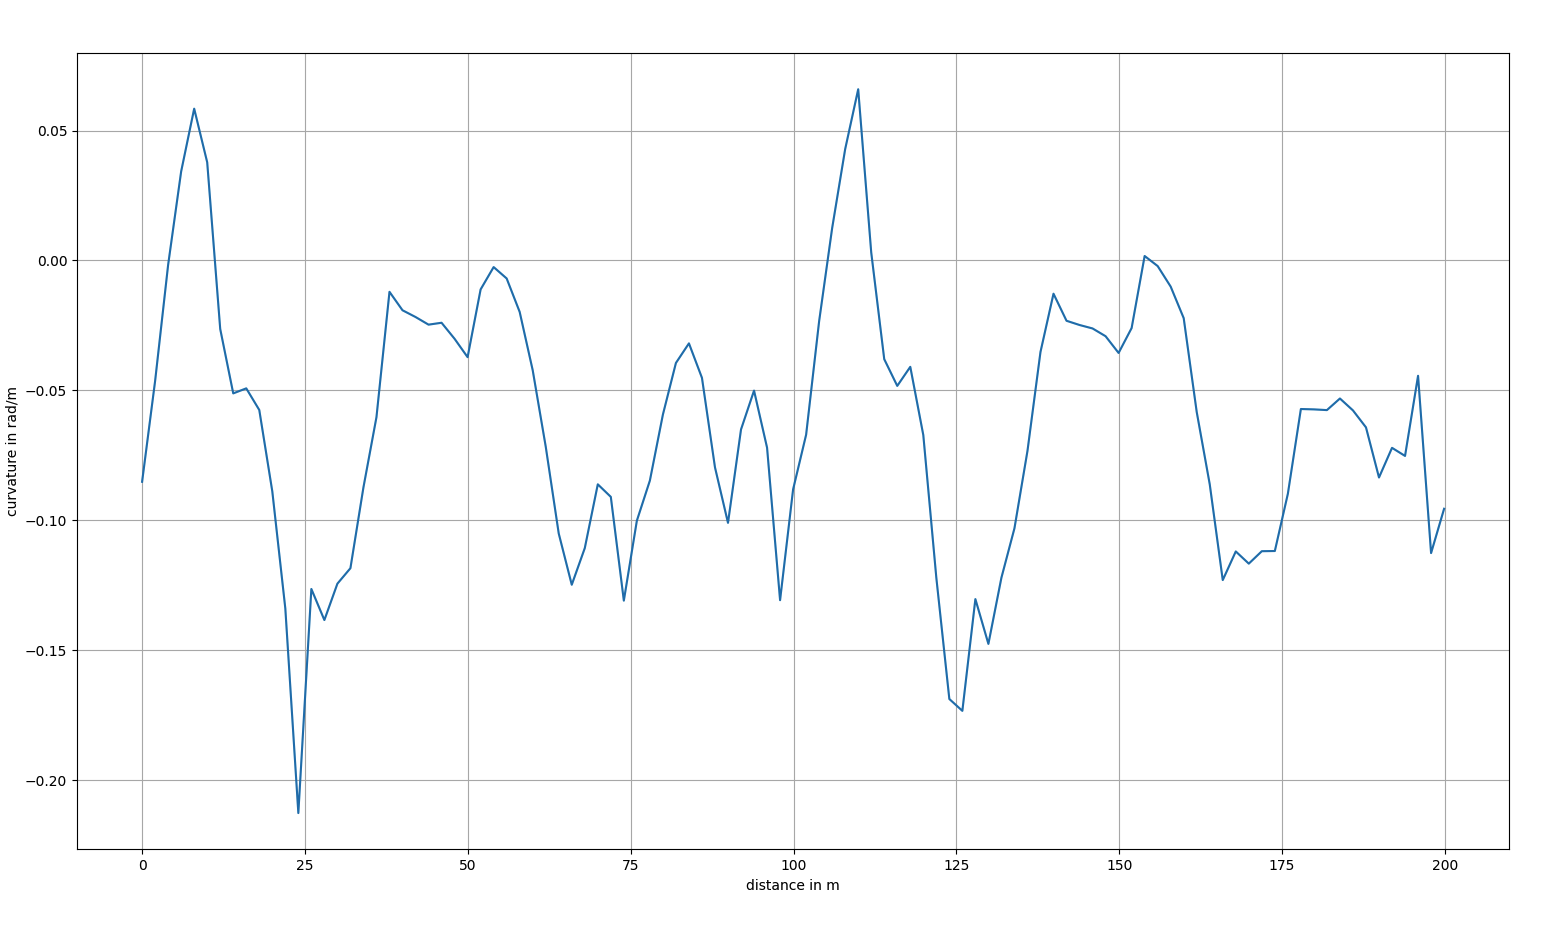
\includegraphics[width=\columnwidth]{Results_Optimization_Small_Track_Laps_2_Curv_Profile.png}
    \caption{The Curvature Profile on Small Track for two laps.}
    \label{fig:Results Small Track Laps 2 Curv Profile}
\end{figure}
\begin{figure}[H]
    \centering
    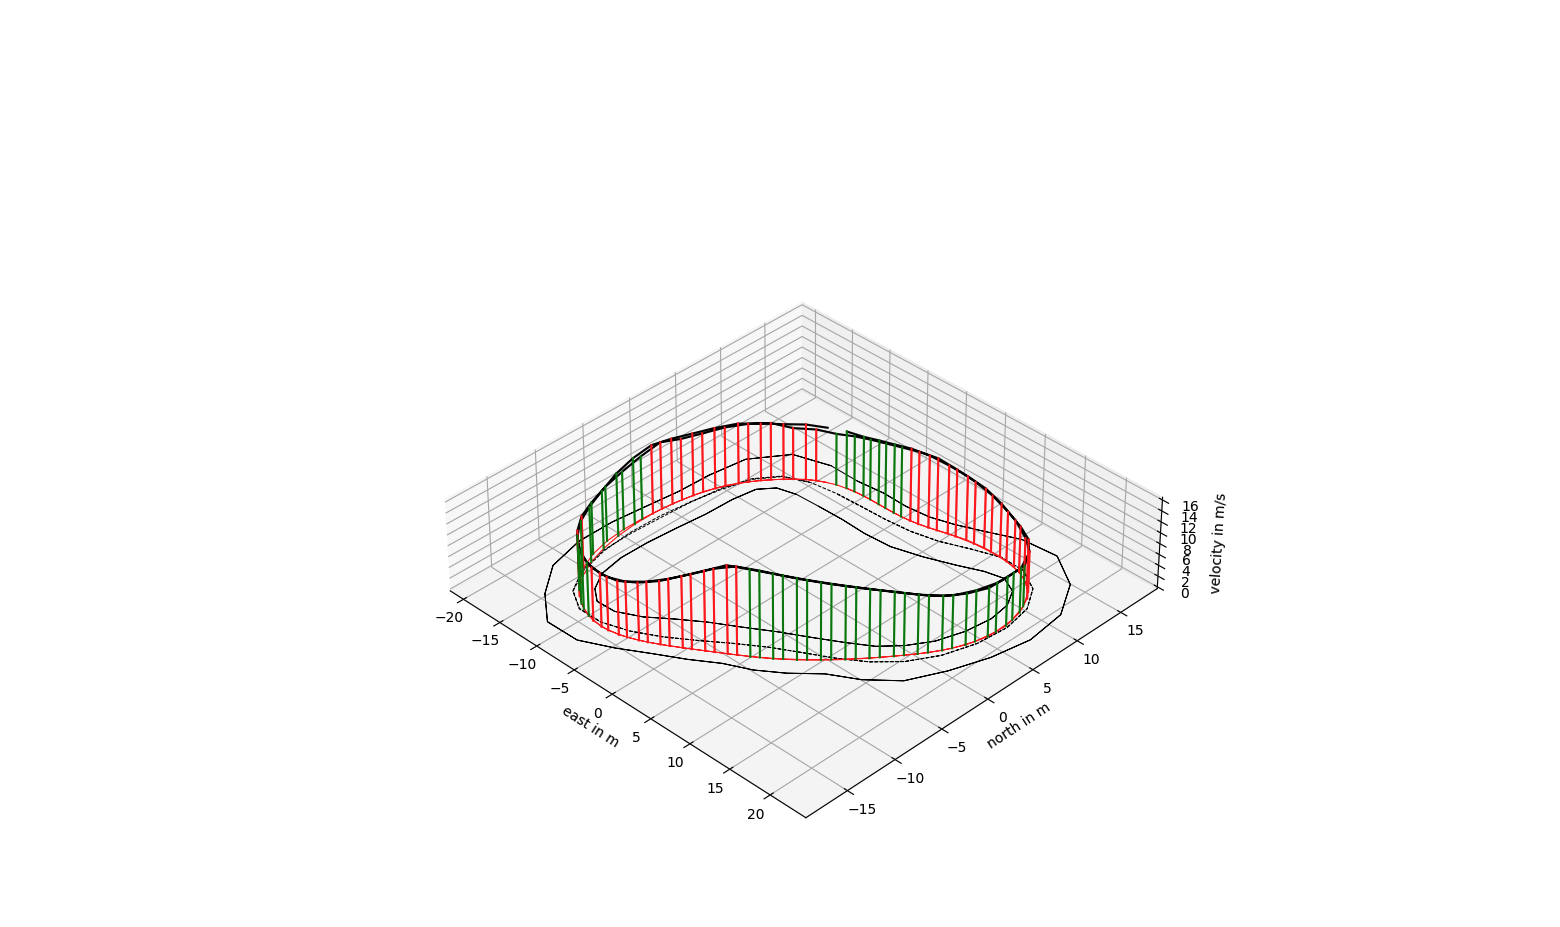
\includegraphics[width=\columnwidth]{Results_Optimization_Small_Track_Laps_2_3D_Vel_Profile.png}
    \caption{The 3D Velocity Profile on Small Track for two laps.}
    \label{fig:Results Small Track Laps 2 3D Vel Profile}
\end{figure}
\begin{figure}[H]
    \centering
    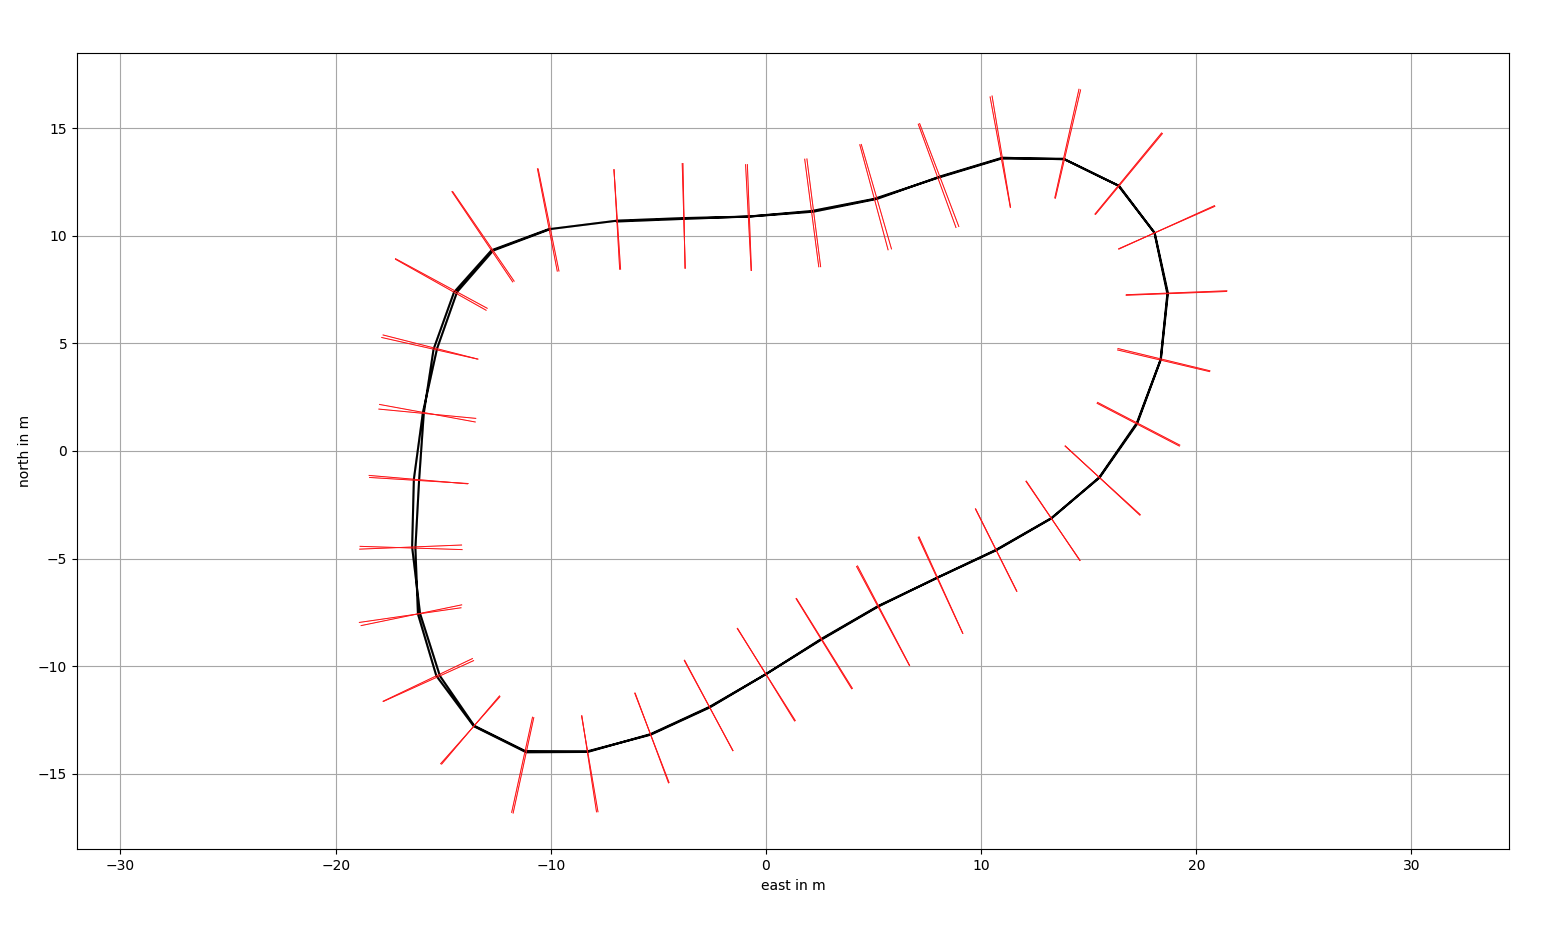
\includegraphics[width=\columnwidth]{Results_Optimization_Small_Track_Laps_2_Spline_Normals.png}
    \caption{The Spline Normals on Small Track for two laps.}
    \label{fig:Results Small Track Laps 2 Spline Normals}
\end{figure}

\section{Rand Track} \label{sec:Results Rand Track}
An overview of the track is shown in figure \ref{fig:Results Rand Initial}. The track was created by the \acrshort{eufs} team too and is called ``Rand''. \cite{eufs_sim_gitlab} It has more cones and curvature than the ``Small Track'' and shows an example of a track that could have been used for the Track Drive event in the competition, as described in section \ref{sec:Dynamic Events}. The track consists of 99 blue cones and 109 yellow cones for the track limits, and 4 big orange cones for the start respectively the end of the track.
\begin{figure}[H]
    \centering
    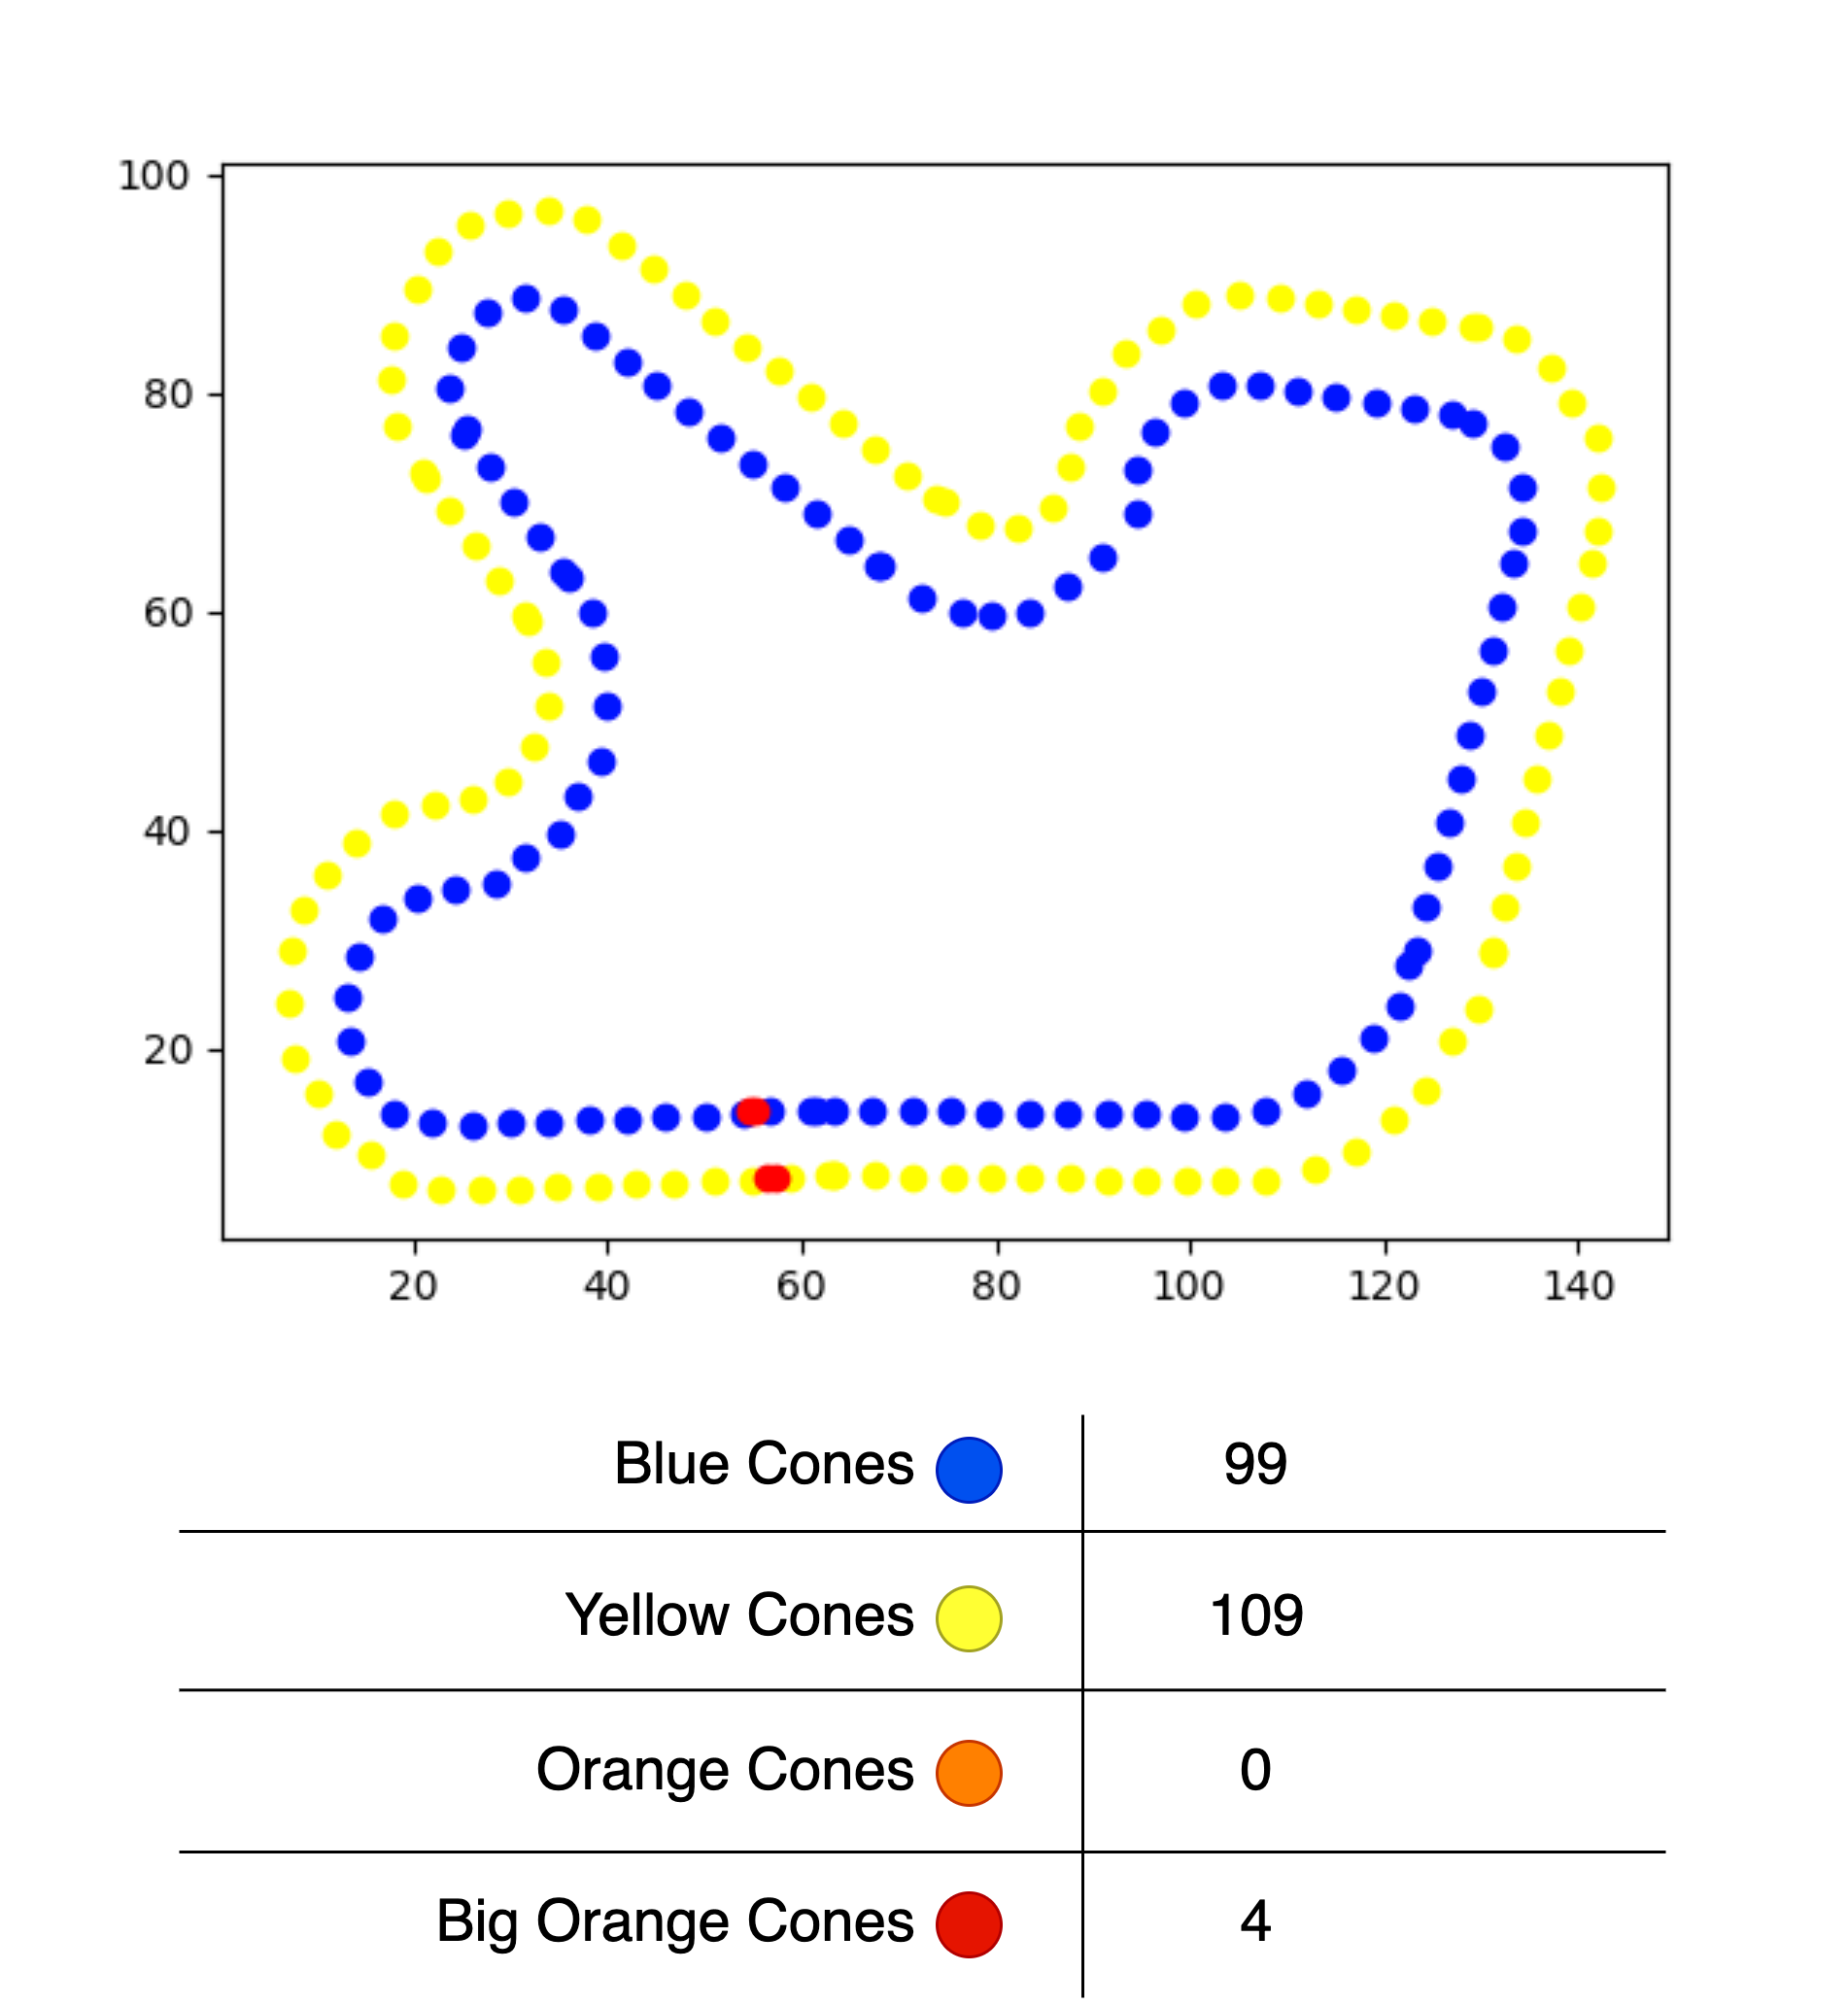
\includegraphics[width=\columnwidth]{Results_Rand_Initial.png}
    \caption{Overview of the Rand Track.}
    \label{fig:Results Rand Initial}
\end{figure}

\textbf{Exploration Algorithm}

During the run with the ``Rand'' track, the algorithm did 215 cycles with a total computation time of 0.6730 seconds. The average cycle lasted 0.0031 seconds, with the fastest cycle taking under < 0.0000 seconds long and the slowest cycle taking 0.0072 seconds long. The algorithm created 2635 reference points during the run. The results are listed in table \ref{tab:Results Rand Exploration}.

\begin{table}[H]
    \centering
    \begin{tabular}{|l|l|l|}
        \hline
        \textbf{Result}            & \textbf{Value} \\ \hline
        Minimum Cycle Time         & < 0.0000 s     \\ \hline
        Maximum Cycle Time         & 0.0072 s       \\ \hline
        Average Cycle  Time        & 0.0031 s       \\ \hline
        Total Cycle Time           & 0.6730 s       \\ \hline
        Number of Cycles           & 215            \\ \hline
        Generated Reference Points & 2635           \\ \hline
    \end{tabular}
    \caption{Results of the Exploration Algorithm on Rand.}
    \label{tab:Results Rand Exploration}
\end{table}

Figure \ref{fig:Result Rand Final} shows the final version of the algorithm on the ``Rand'' track.
\begin{figure}[H]
    \centering
    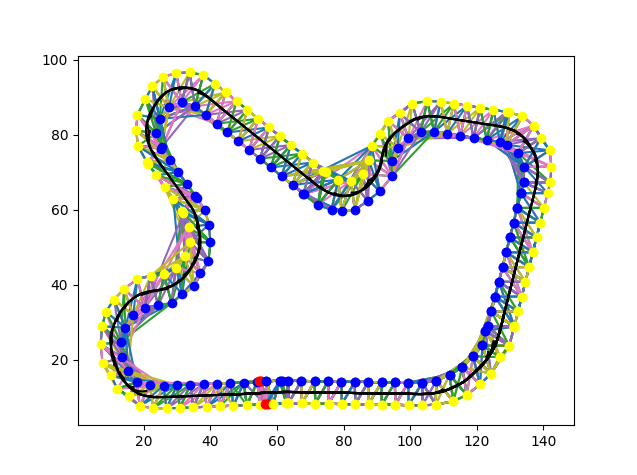
\includegraphics[width=\columnwidth]{Result_Rand_final.png}
    \caption{The ``Rand'' track with the final algorithm implementation.}
    \label{fig:Result Rand Final}
\end{figure}

\textbf{Optimization Algorithm}

A comparison of the different objectives on the Rand track is given in table \ref{tab:Results Rand Optimization Objectives}. Two laps on the given track were calculated for each objective: Shortest Path, Minimum Curvature and Minimum Curvature with iterative call. The result with the Shortest Path objective is seen in figure \ref{fig:Results Rand Laps 2 Shortest Path}, the result with the Minimum Curvature objective is seen in figure \ref{fig:Results Rand Laps 2 Minimum Curvature}, and the result with the Minimum Curvature objective with an iterative call is seen in figure \ref{fig:Results Rand Laps 2 Minimum Curvature IQP}.

\begin{table}[H]
    \centering
    \begin{tabular}{|l|l|l|l|}
        \hline
        \textbf{Objective}    & \textbf{Runtime} & \textbf{Estimated Lap Time} & \textbf{Generated Reference Points} \\ \hline
        Shortest Path         & 0.28 s           & 60.84 s                     & 376 Reference Points                \\ \hline
        Minimum Curvature     & 0.37 s           & 49.83 s                     & 388 Reference Points                \\ \hline
        Minimum Curvature IQP & 0.82 s           & 47.80 s                     & 384 Reference Points                \\ \hline
    \end{tabular}
    \caption{Results of the different Optimization Algorithm objectives on Rand for two laps.}
    \label{tab:Results Rand Optimization Objectives}
\end{table}
\begin{figure}[H]
    \centering
    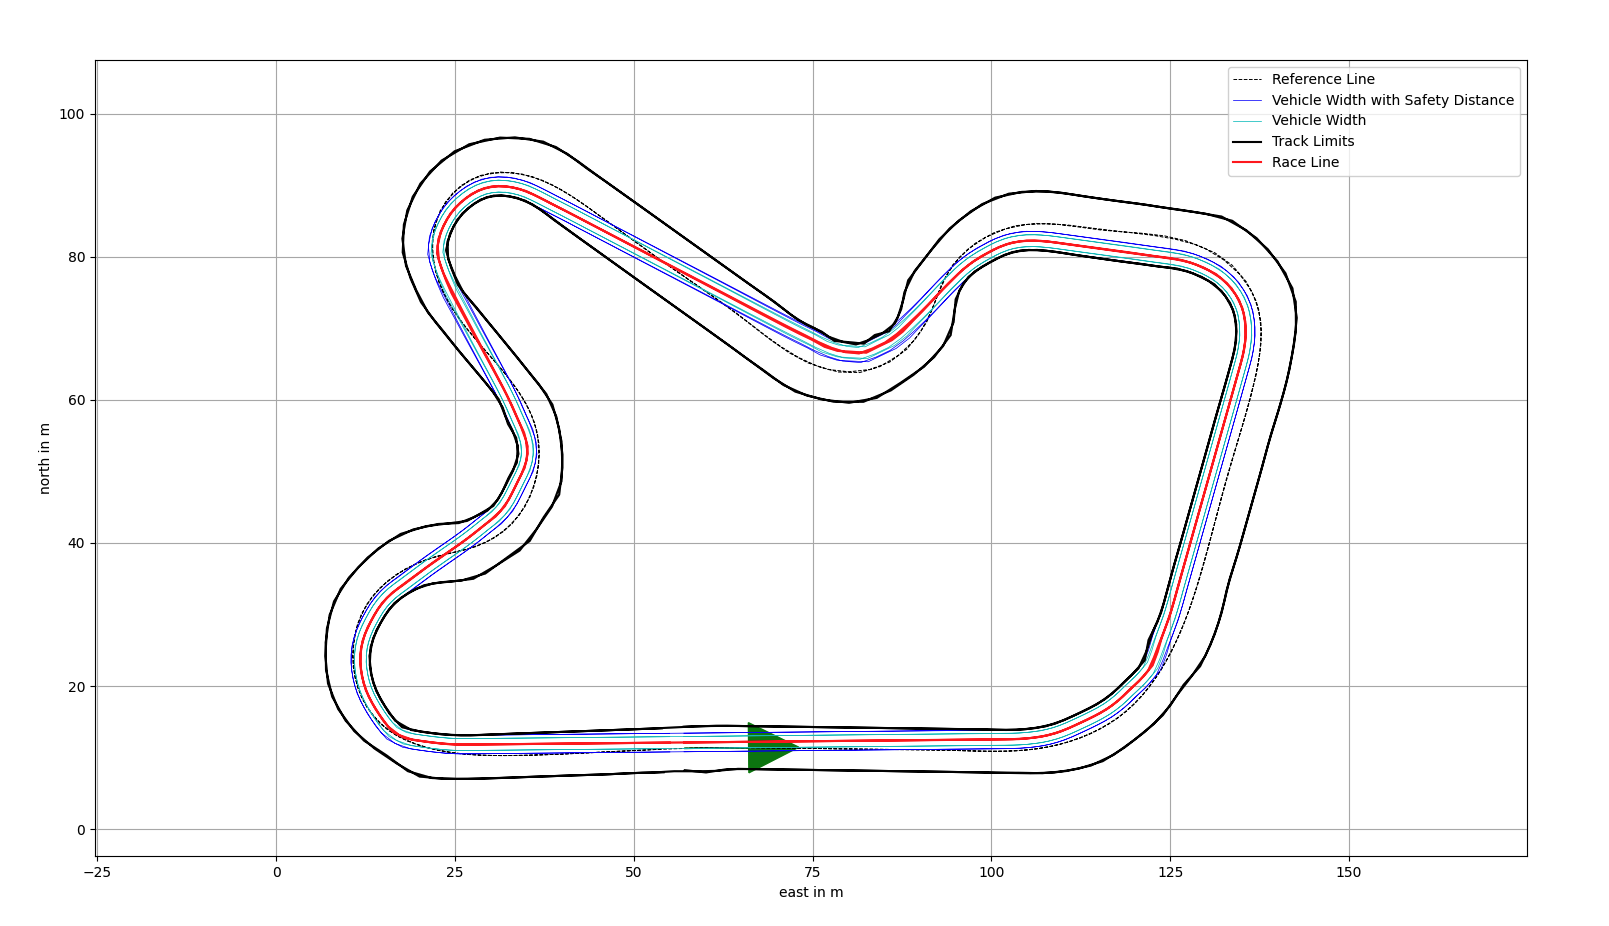
\includegraphics[width=\columnwidth]{Results_Optimization_Rand_Laps_2_Shortest_Path.png}
    \caption{Optimization on the Rand track for two laps with the Shortest Path objective.}
    \label{fig:Results Rand Laps 2 Shortest Path}
\end{figure}
\begin{figure}[H]
    \centering
    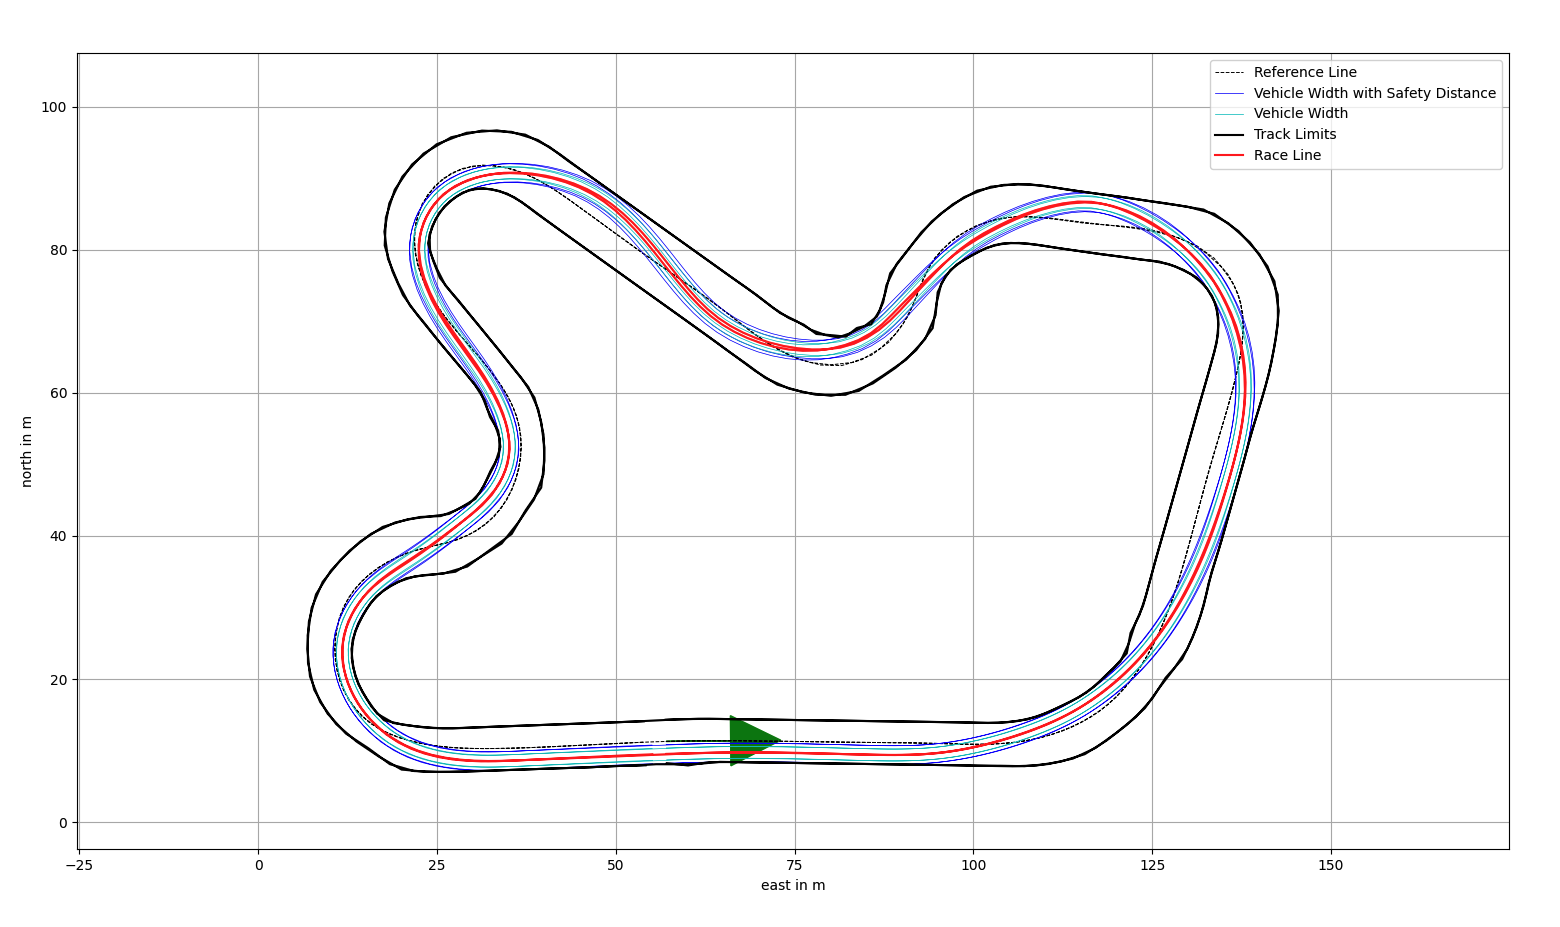
\includegraphics[width=\columnwidth]{Results_Optimization_Rand_Laps_2.png}
    \caption{Optimization on the Rand track for two laps with the Minimum Curvature objective.}
    \label{fig:Results Rand Laps 2 Minimum Curvature}
\end{figure}
\begin{figure}[H]
    \centering
    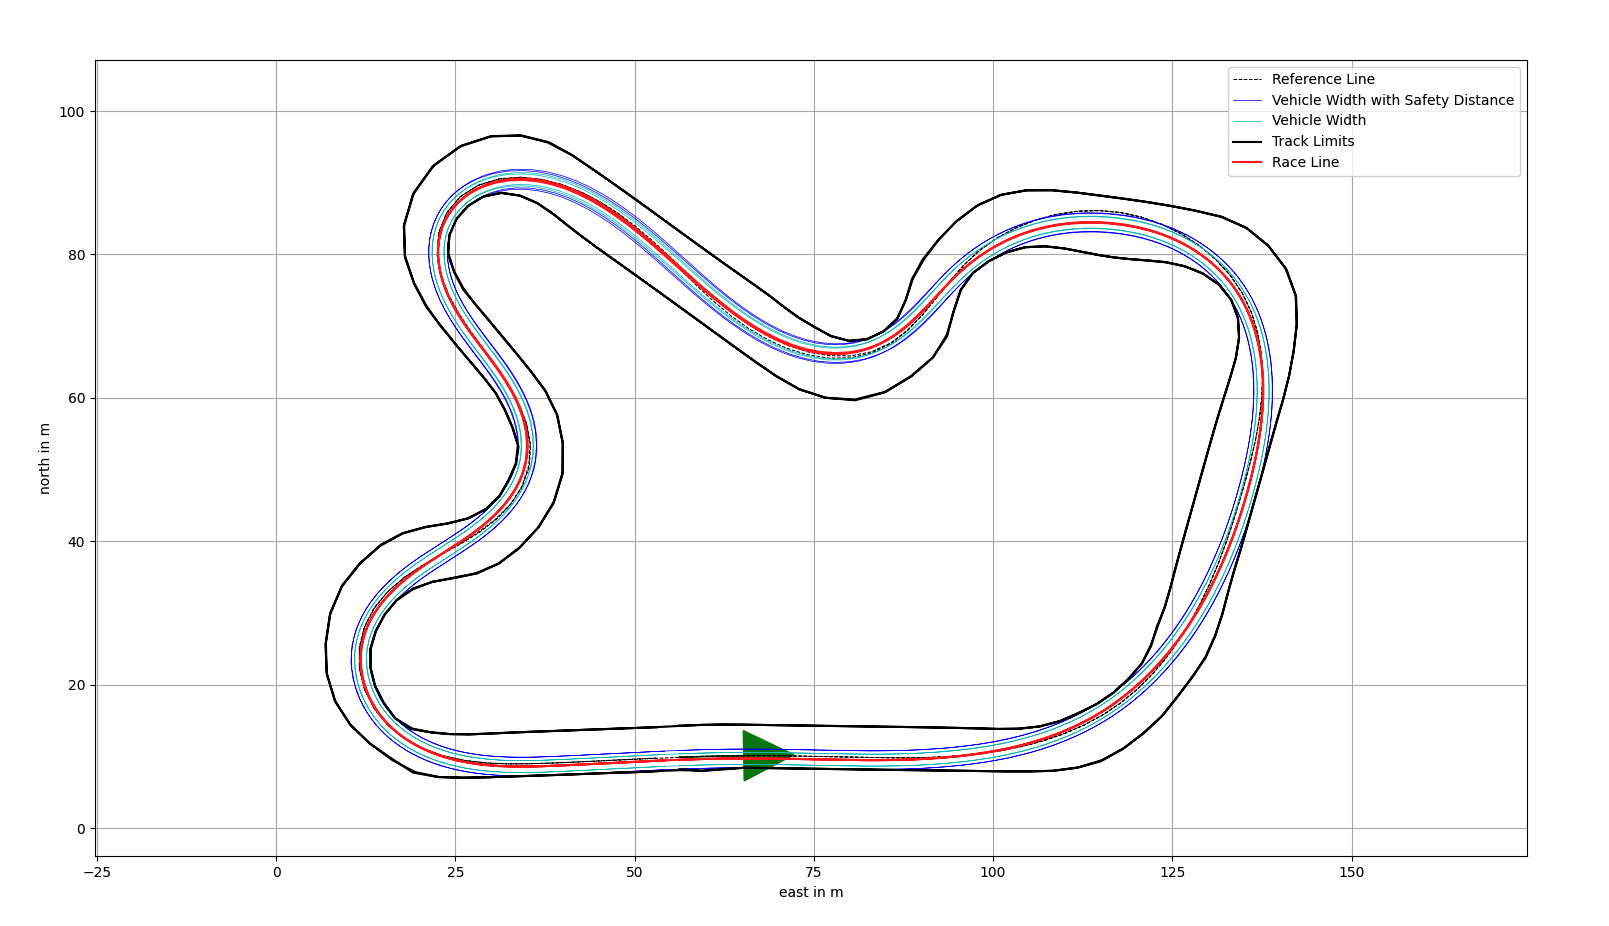
\includegraphics[width=\columnwidth]{Results_Optimization_Rand_Laps_2_Mincurv_IQP.png}
    \caption{Optimization on the Rand track for two laps with the Minimum Curvature objective with iterative call.}
    \label{fig:Results Rand Laps 2 Minimum Curvature IQP}
\end{figure}

The results for the Optimization Algorithm with the Minimum Curvature objective for one lap, two laps, three laps, five laps and eight laps are detailed in table \ref{tab:Results Rand Optimization Laps 1-8}. The visual comparison of the output between one lap, three laps, five laps and eight laps is shown in figure \ref{fig:Results Rand Laps 1-8}.

\begin{table}[H]
    \centering
    \begin{tabular}{|l|l|l|l|}
        \hline
        \textbf{Laps} & \textbf{Runtime} & \textbf{Estimated Lap Time} & \textbf{Generated Reference Points} \\ \hline
        1             & 0.12 s           & 24.76 s                     & 194 Reference Points                \\ \hline
        2             & 0.37 s           & 49.83 s                     & 388 Reference Points                \\ \hline
        3             & 0.92 s           & 75.69 s                     & 581 Reference Points                \\ \hline
        5             & 3.41 s           & 129.65 s                    & 967 Reference Points                \\ \hline
        8             & 13.18 s          & 219.83 s                    & 1546 Reference Points               \\ \hline
    \end{tabular}
    \caption{Results of the Optimization Algorithm with the Minimum Curvature objective on Small Track for one to eight laps.}
    \label{tab:Results Rand Optimization Laps 1-8}
\end{table}
\begin{figure}[H]
    \centering
    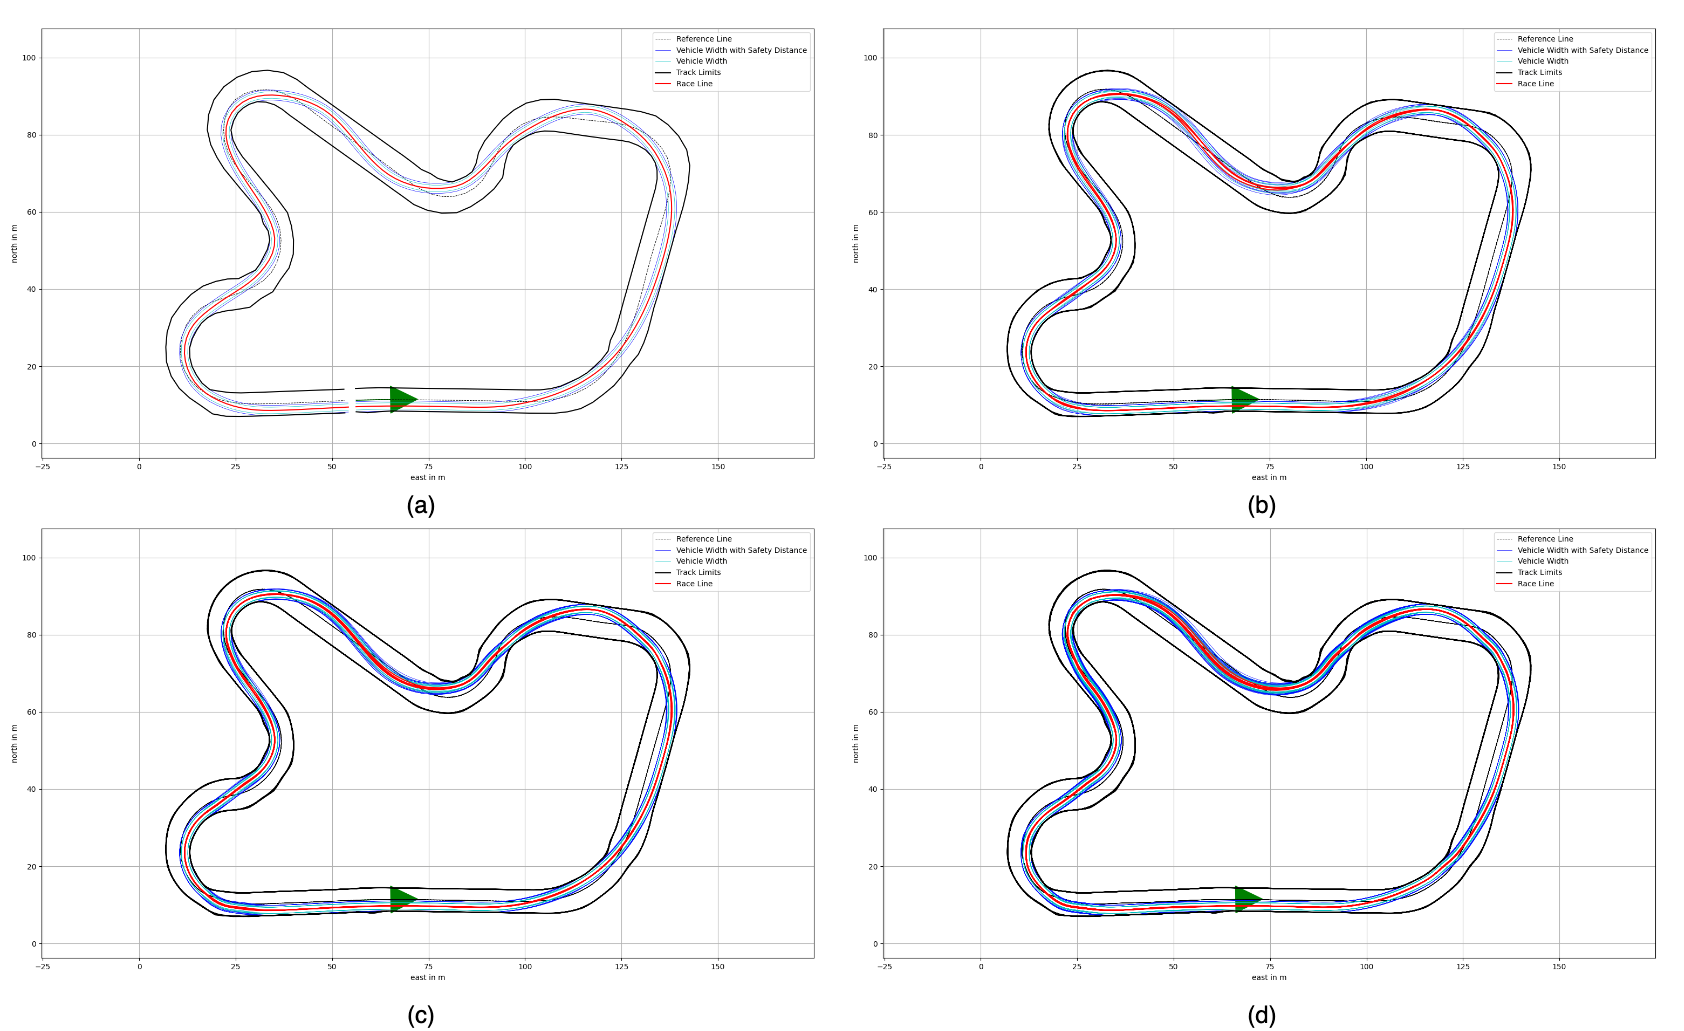
\includegraphics[width=\columnwidth]{Results_Optimization_Rand_Laps_1-8.png}
    \caption{Optimization on the Rand track with the Minimum Curvature objective for one lap (a), three laps (b), five laps (c), and eight laps (d).}
    \label{fig:Results Rand Laps 1-8}
\end{figure}

Additionally, the following outputs of the Optimization Algorithm with the Minimum Curvature objective for two laps on the Rand track are shown: The Velocity and Acceleration Profile in figure \ref{fig:Results Rand Laps 2 VelAcc Profile}, the Curvature Profile in figure \ref{fig:Results Rand Laps 2 Curv Profile}, the 3D Velocity Profile in figure \ref{fig:Results Rand Laps 2 3D Vel Profile}, and the Spline Normals in figure \ref{fig:Results Rand Laps 2 Spline Normals}.
\begin{figure}[H]
    \centering
    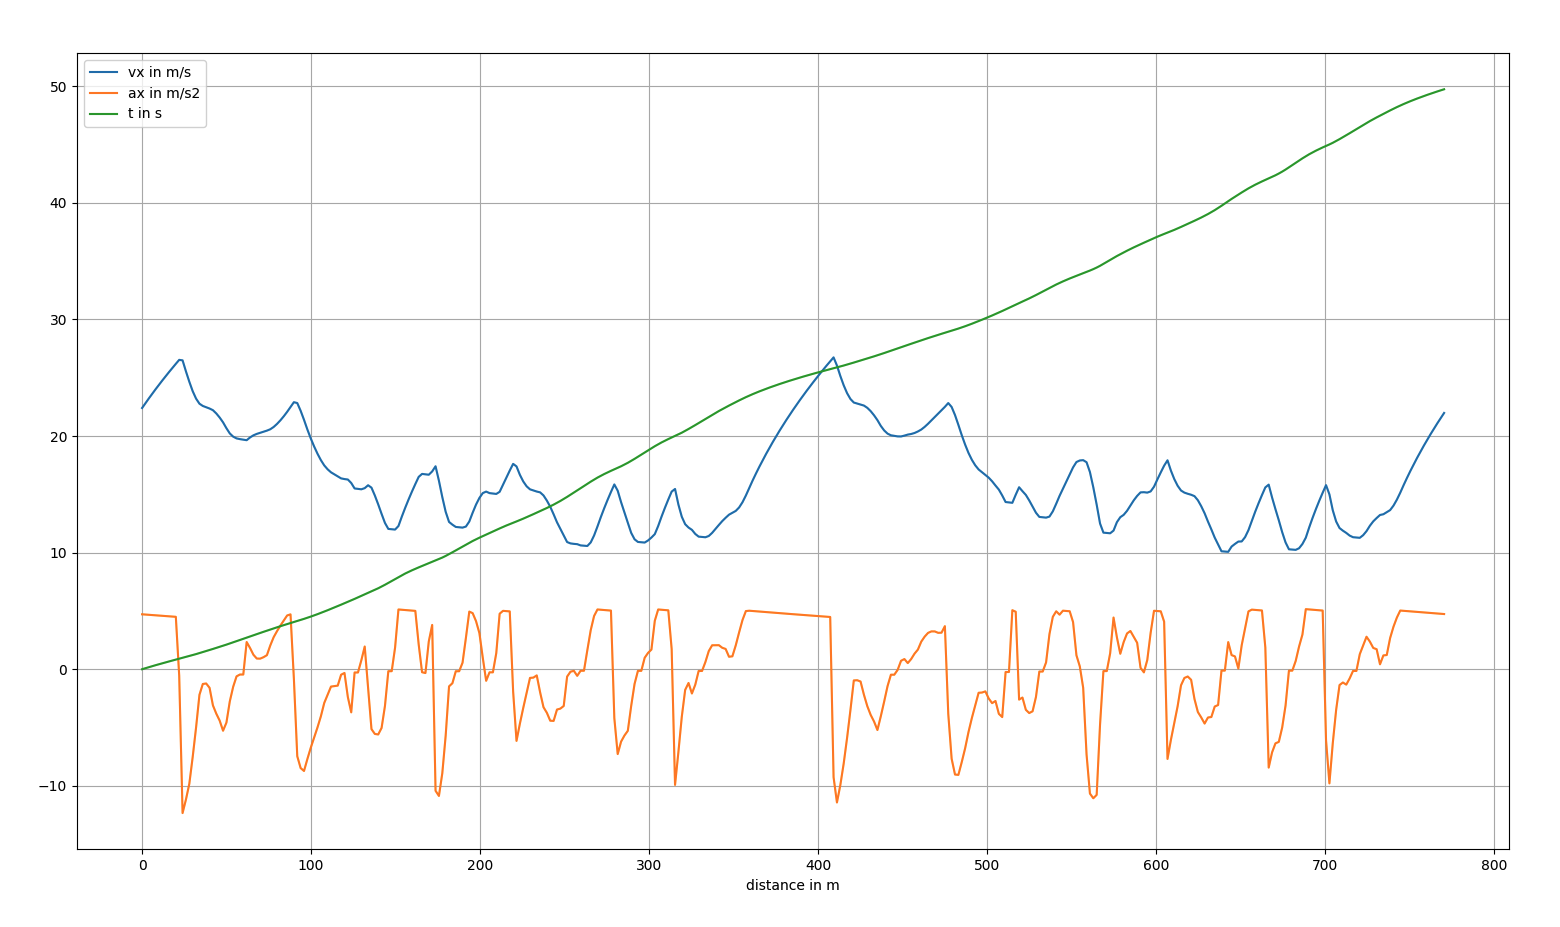
\includegraphics[width=\columnwidth]{Results_Optimization_Rand_Laps_2_VelAcc_Profile.png}
    \caption{The Velocity and Acceleration Profile on Rand for two laps.}
    \label{fig:Results Rand Laps 2 VelAcc Profile}
\end{figure}
\begin{figure}[H]
    \centering
    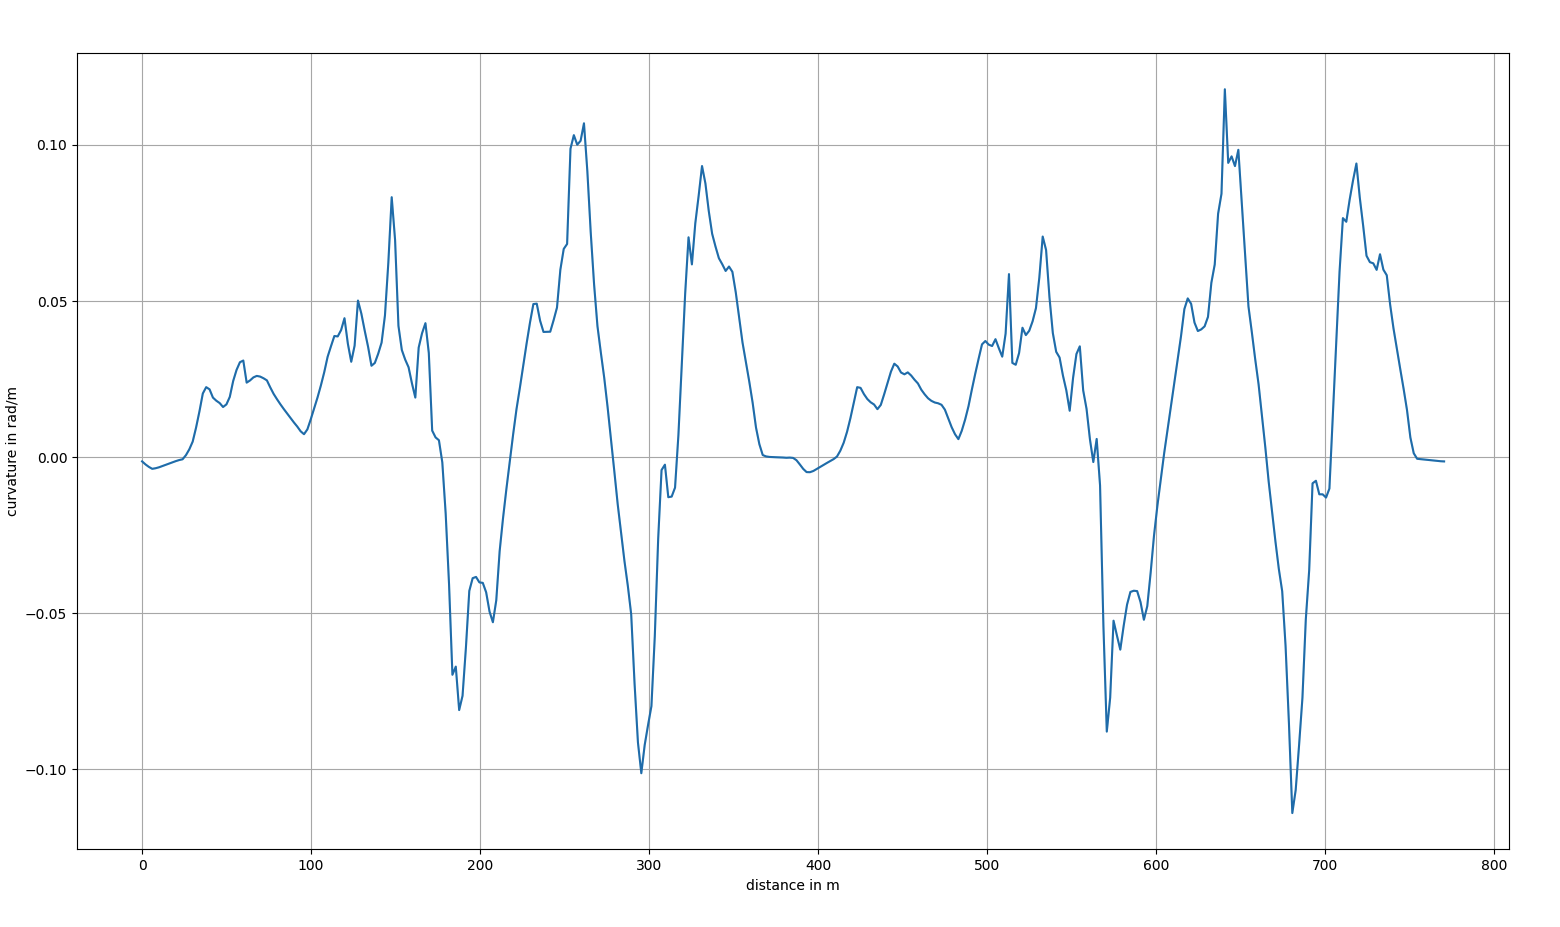
\includegraphics[width=\columnwidth]{Results_Optimization_Rand_Laps_2_Curv_Profile.png}
    \caption{The Curvature Profile on Rand for two laps.}
    \label{fig:Results Rand Laps 2 Curv Profile}
\end{figure}
\begin{figure}[H]
    \centering
    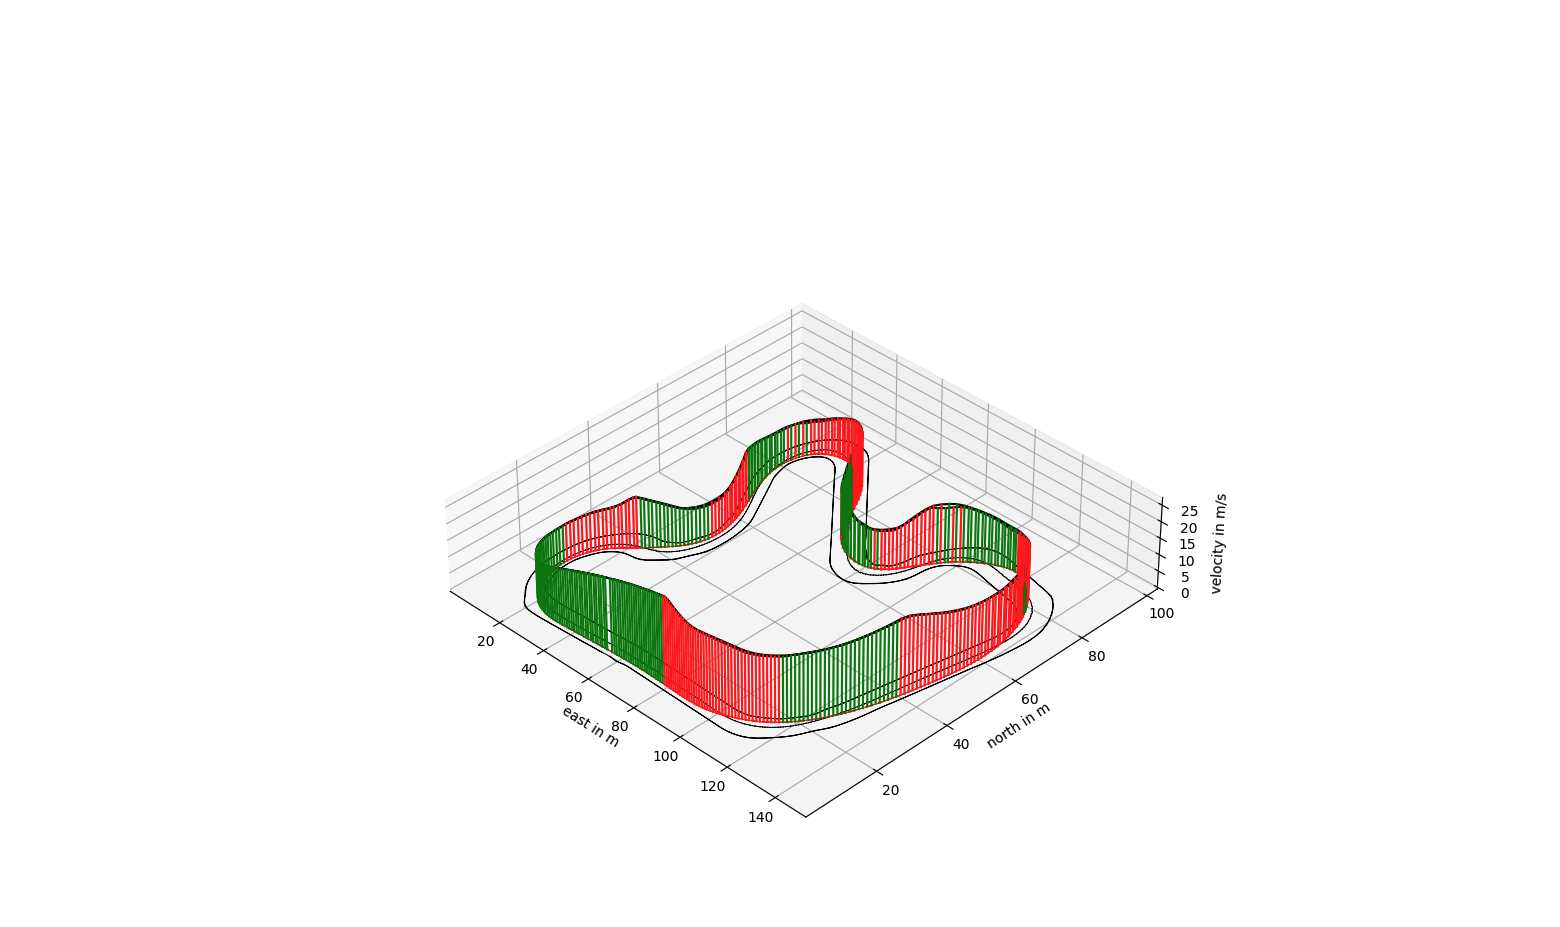
\includegraphics[width=\columnwidth]{Results_Optimization_Rand_Laps_2_3D_Vel_Profile.png}
    \caption{The 3D Velocity Profile on Rand for two laps.}
    \label{fig:Results Rand Laps 2 3D Vel Profile}
\end{figure}
\begin{figure}[H]
    \centering
    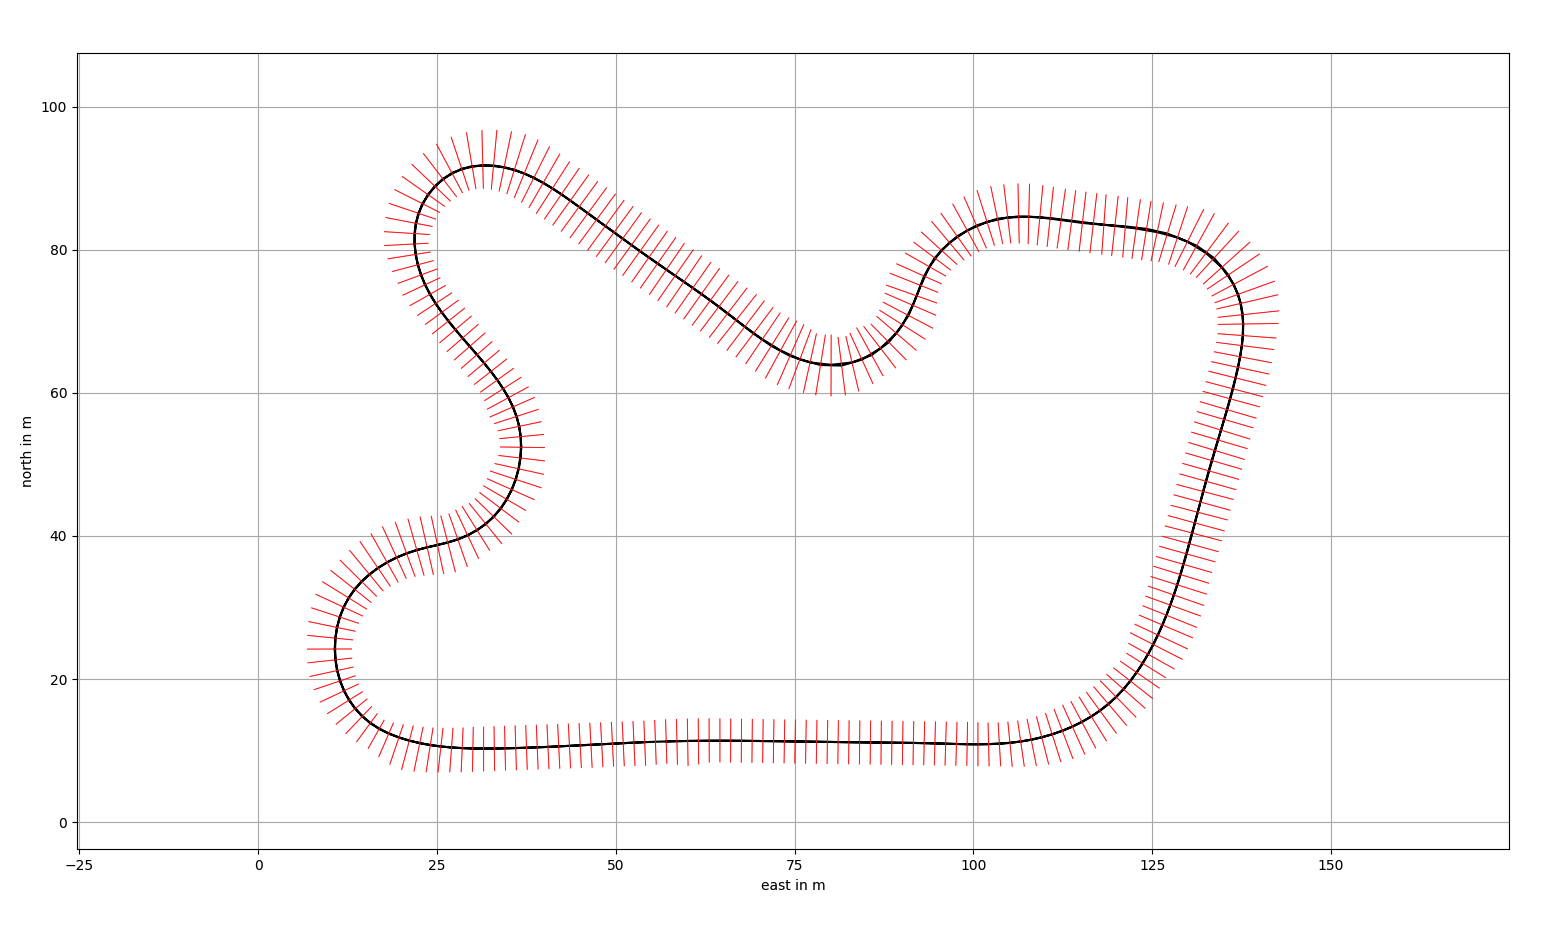
\includegraphics[width=\columnwidth]{Results_Optimization_Rand_Laps_2_Spline_Normals.png}
    \caption{The Spline Normals on Rand for two laps.}
    \label{fig:Results Rand Laps 2 Spline Normals}
\end{figure}

\section{Competition 2021 Track} \label{sec:Results Competition 2021 Track}
An overview of the track is shown in figure \ref{fig:Results Comp 2021 Initial}. The track was created by the \acrshort{eufs} team too and is called ``Comp 2021''. \cite{eufs_sim_gitlab} The track was used for a competition in 2021 and consists of more corners than the ``Rand'' track. The track consists of 156 blue cones and 156 yellow cones for the track limits, and 4 big orange cones for the start respectively the end of the track.
\begin{figure}[H]
    \centering
    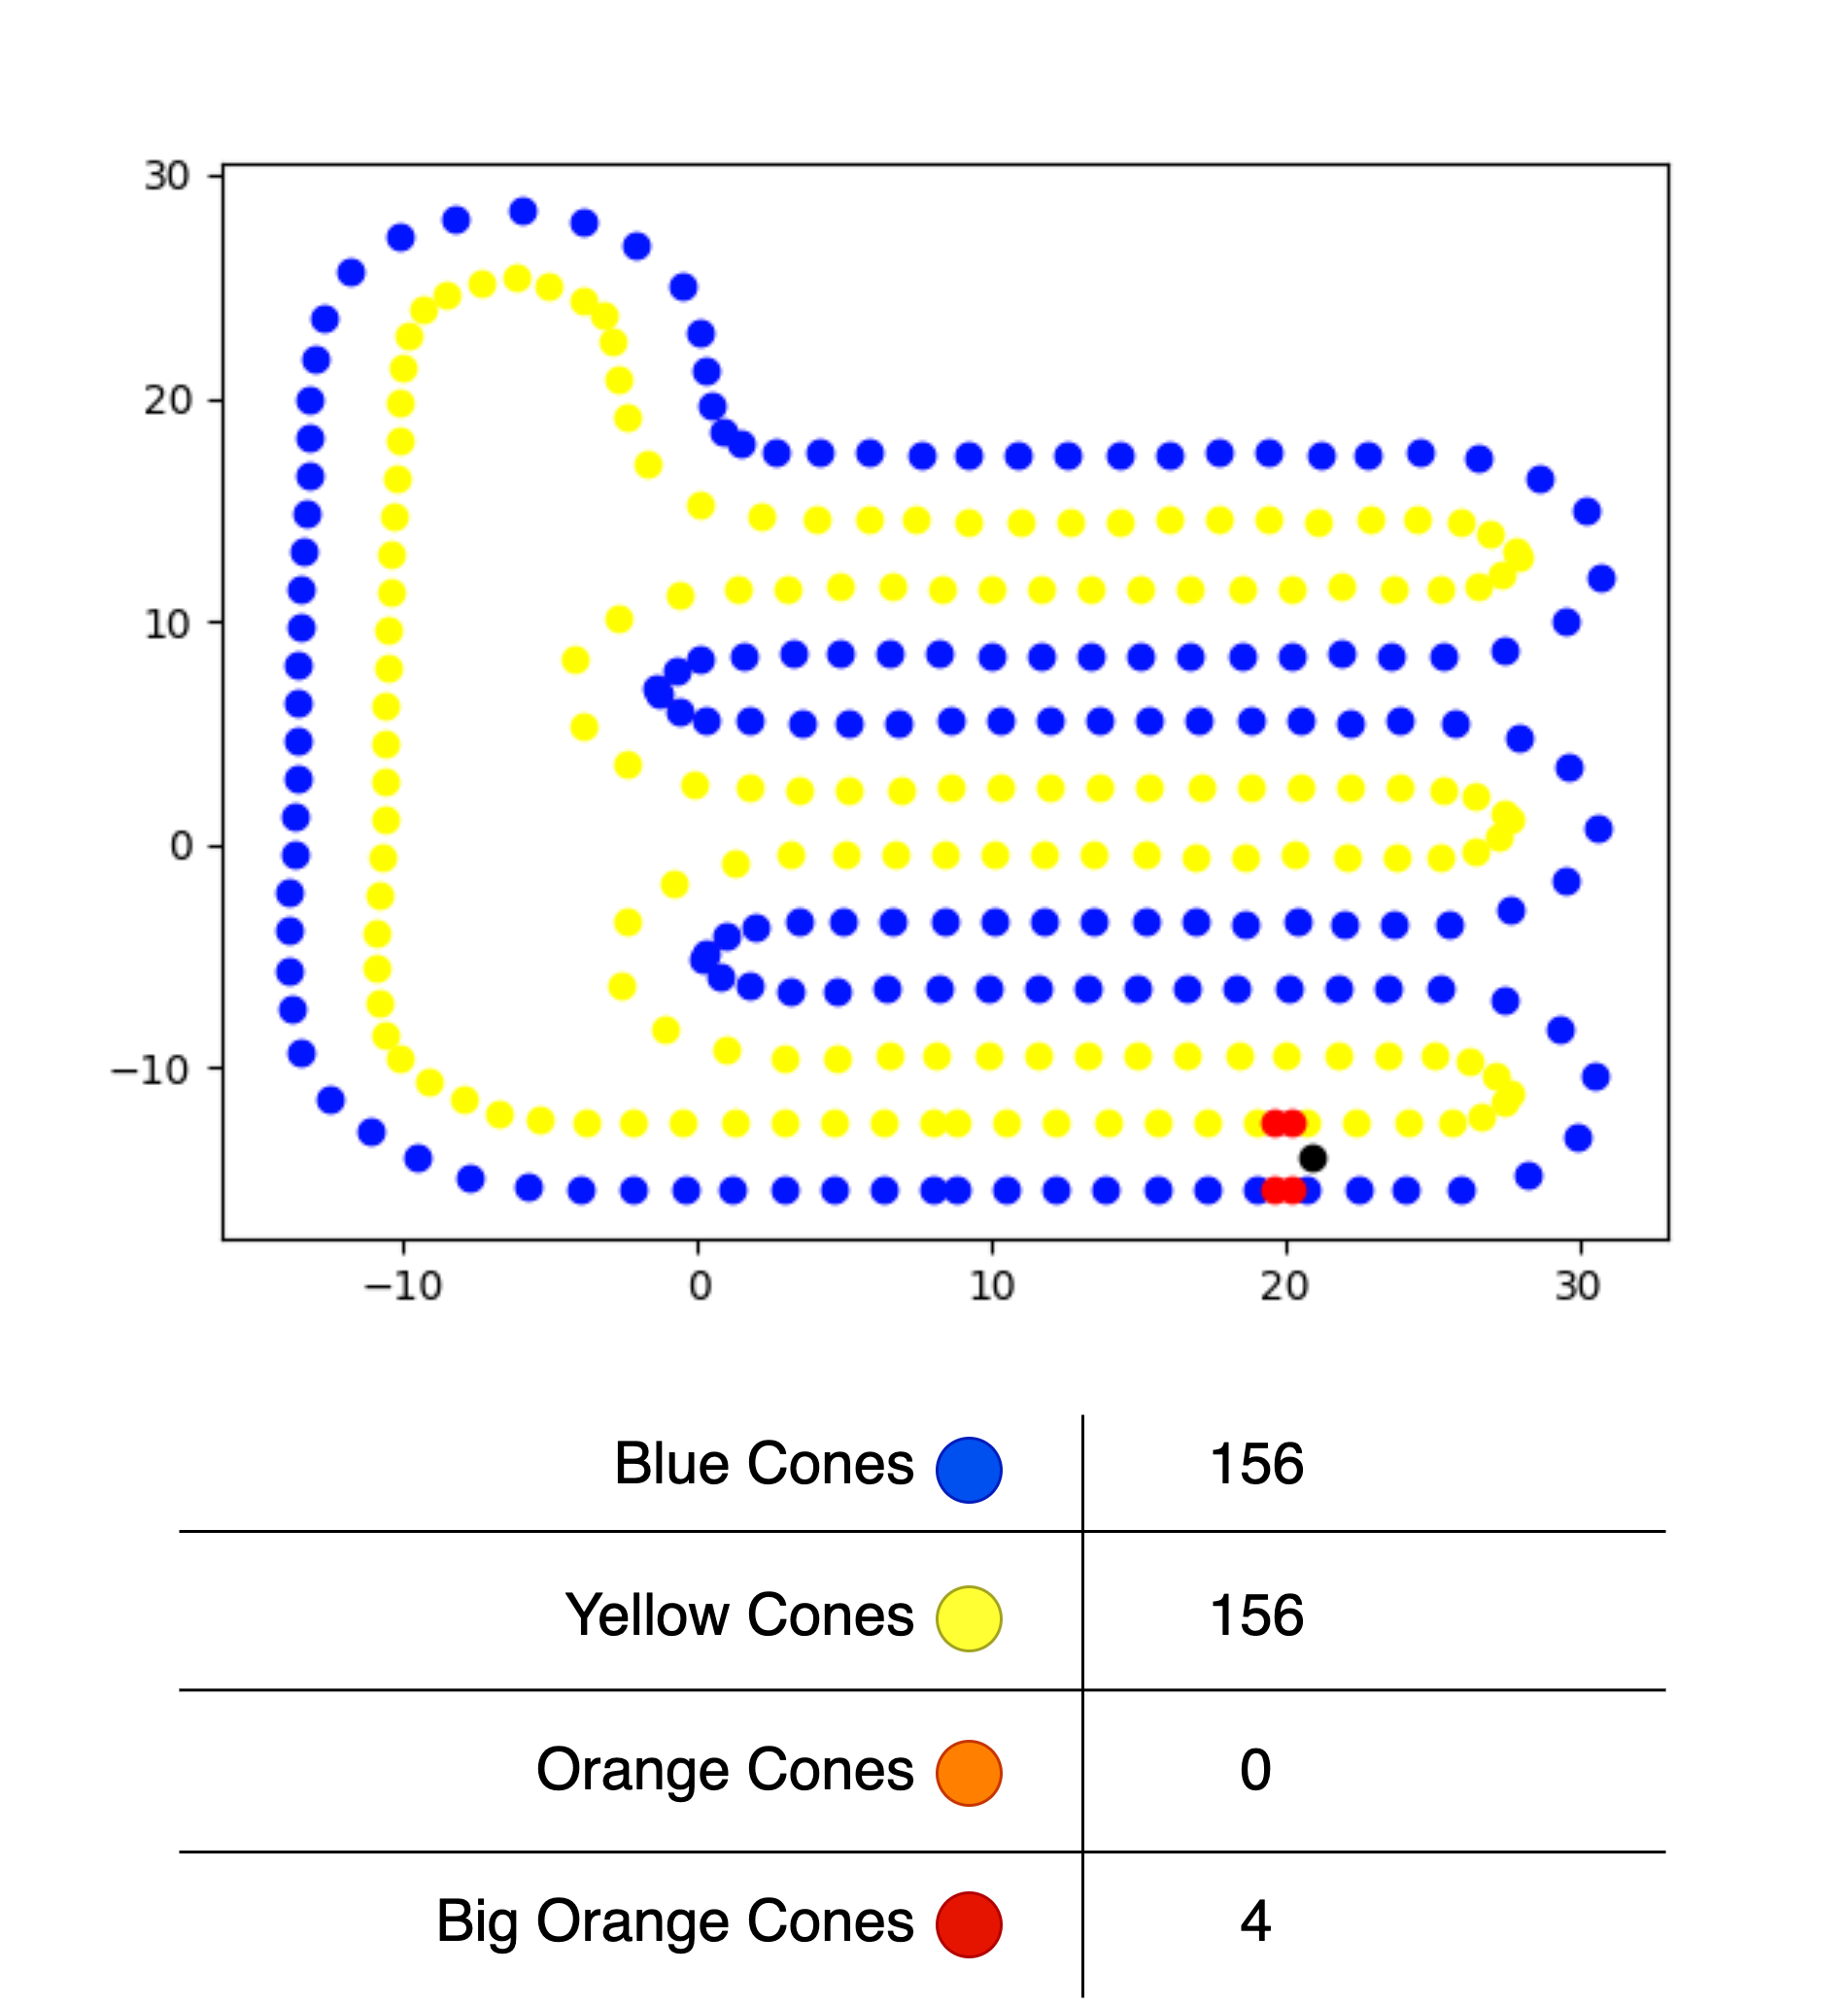
\includegraphics[width=\columnwidth]{Results_Comp_2021_Initial.png}
    \caption{Overview of the Competition 2021 Track.}
    \label{fig:Results Comp 2021 Initial}
\end{figure}

\textbf{Exploration Algorithm}

During the run with the ``Comp 2021'' track, the algorithm did 320 cycles with a total computation time of 0.6621 seconds. The average cycle lasted 0.0021 seconds, with the fastest cycle taking under < 0.0000 seconds long and the slowest cycle taking 0.0069 seconds long. The algorithm created 3425 reference points during the run. The results are listed in table \ref{tab:Results Comp 2021 Exploration}.

\begin{table}[H]
    \centering
    \begin{tabular}{|l|l|l|}
        \hline
        \textbf{Result}            & \textbf{Value} \\ \hline
        Minimum Cycle Time         & < 0.0000 s     \\ \hline
        Maximum Cycle Time         & 0.0072 s       \\ \hline
        Average Cycle  Time        & 0.0031 s       \\ \hline
        Total Cycle Time           & 0.6730 s       \\ \hline
        Number of Cycles           & 215            \\ \hline
        Generated Reference Points & 2635           \\ \hline
    \end{tabular}
    \caption{Results of the Exploration Algorithm on the Competition 2021 track.}
    \label{tab:Results Comp 2021 Exploration}
\end{table}

Figure \ref{fig:Result Comp 2021 Final} shows the final version of the algorithm on the ``Comp 2021'' track.
\begin{figure}[H]
    \centering
    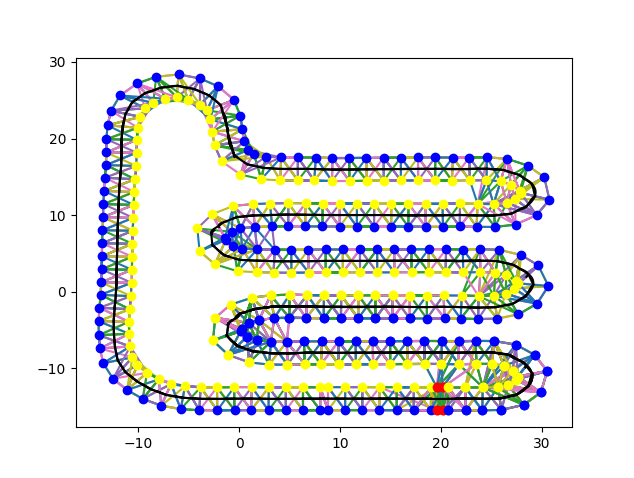
\includegraphics[width=\columnwidth]{Result_Comp2021_final.png}
    \caption{The ``Rand'' track with the final algorithm implementation.}
    \label{fig:Result Comp 2021 Final}
\end{figure}

\textbf{Optimization Algorithm}

A comparison of the different objectives on the Competition 2021 track is given in table \ref{tab:Results Comp 2021 Optimization Objectives}. Two laps on the given track were calculated for each objective: Shortest Path, Minimum Curvature and Minimum Curvature with iterative call. The result with the Shortest Path objective is seen in figure \ref{fig:Results Comp 2021 Laps 2 Shortest Path}, the result with the Minimum Curvature objective is seen in figure \ref{fig:Results Comp 2021 Laps 2 Minimum Curvature}, and the calculation with the Minimum Curvature objective with an iterative call did not finish in a reasonable time.

\begin{table}[H]
    \centering
    \begin{tabular}{|l|l|l|l|}
        \hline
        \textbf{Objective}    & \textbf{Runtime} & \textbf{Estimated Lap Time} & \textbf{Generated Reference Points} \\ \hline
        Shortest Path         & 0.25 s           & 59.29 s                     & 248 Reference Points                \\ \hline
        Minimum Curvature     & 0.30 s           & 58.87 s                     & 259 Reference Points                \\ \hline
        Minimum Curvature IQP & DNF*             & DNF*                        & DNF*                                \\ \hline
    \end{tabular}
    \caption{Results of the different Optimization Algorithm objectives on the Competition 2021 track for two laps. (* Did not finish)}
    \label{tab:Results Comp 2021 Optimization Objectives}
\end{table}
\begin{figure}[H]
    \centering
    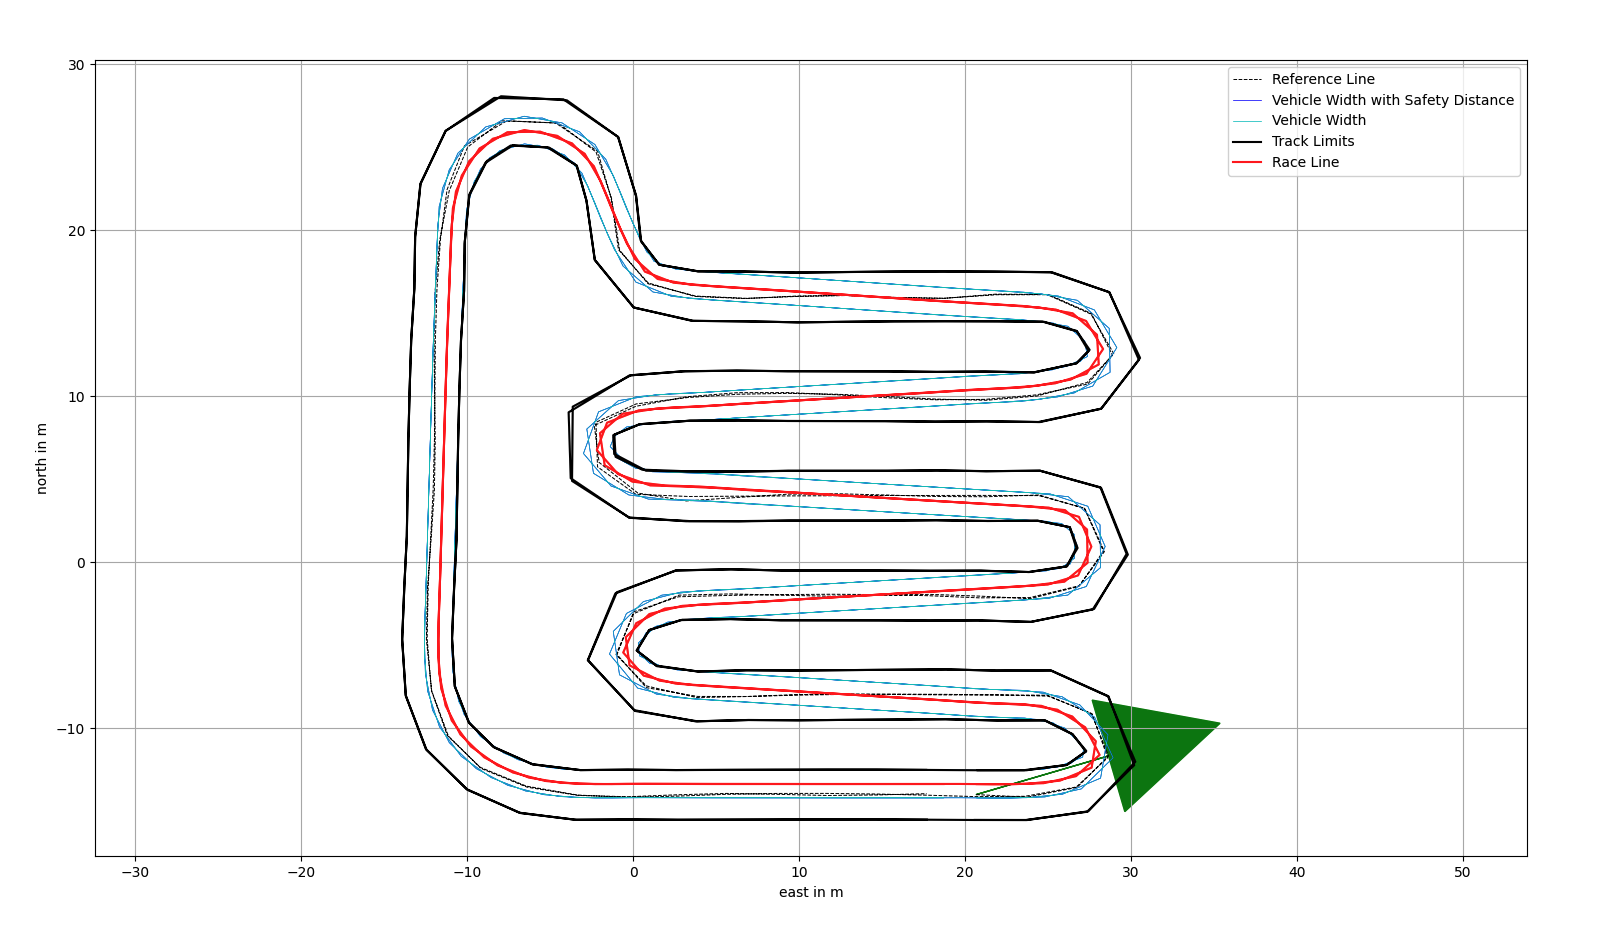
\includegraphics[width=\columnwidth]{Results_Optimization_Comp_2021_Laps_2_Shortest_Path.png}
    \caption{Optimization on the Competition 2021 track for two laps with the Shortest Path objective.}
    \label{fig:Results Comp 2021 Laps 2 Shortest Path}
\end{figure}
\begin{figure}[H]
    \centering
    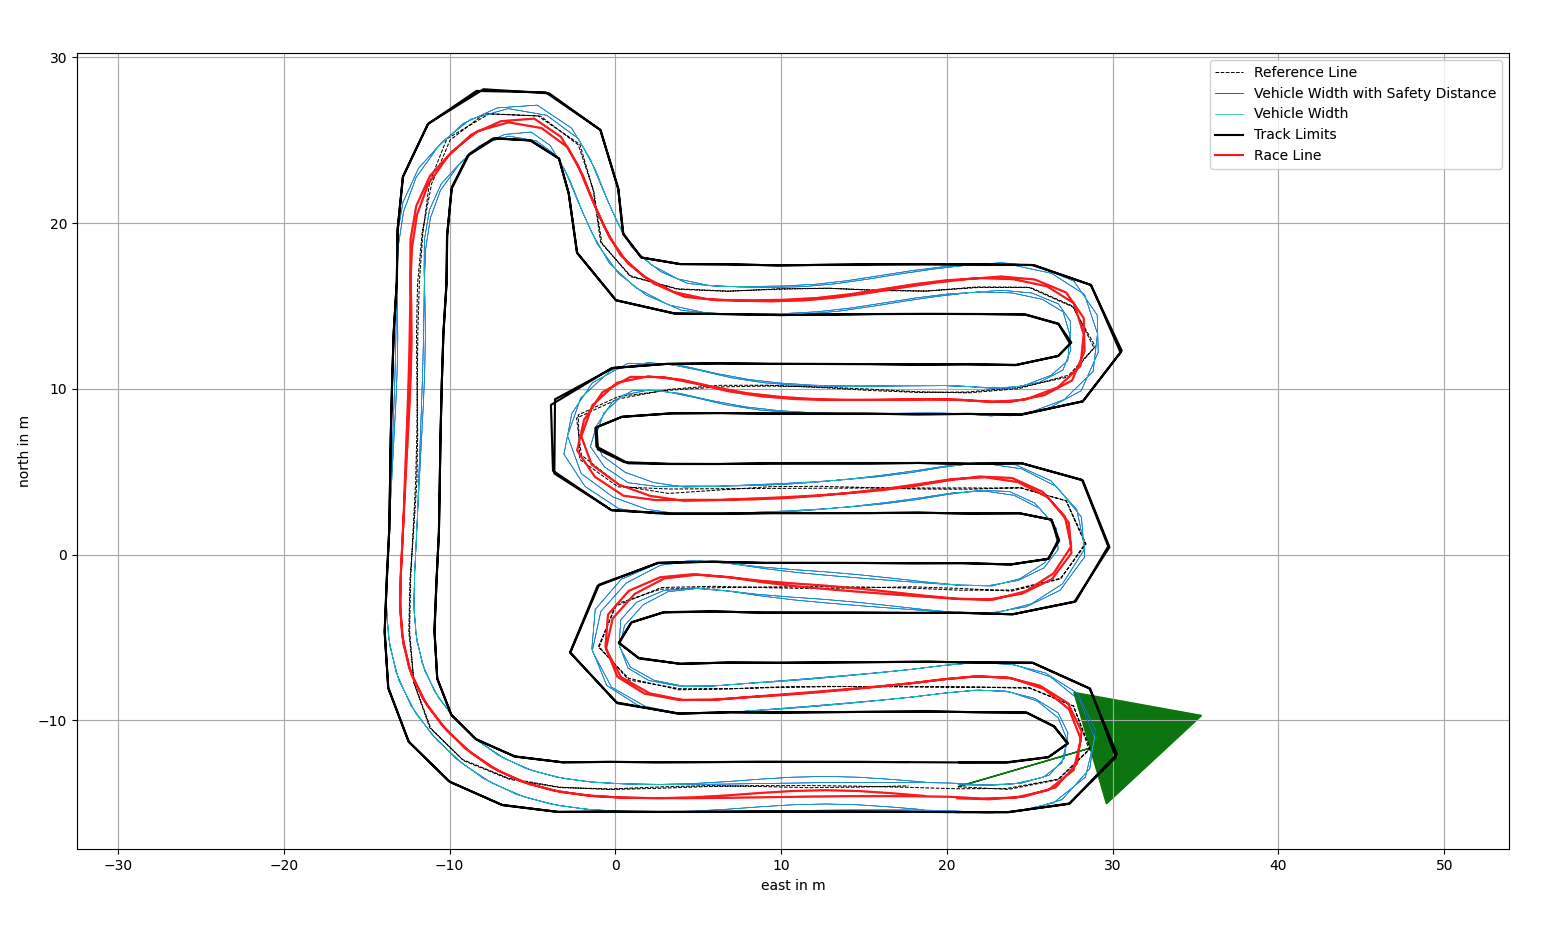
\includegraphics[width=\columnwidth]{Results_Optimization_Comp_2021_Laps_2.png}
    \caption{Optimization on the Competition 2021 track for two laps with the Minimum Curvature objective.}
    \label{fig:Results Comp 2021 Laps 2 Minimum Curvature}
\end{figure}

The results for the Optimization Algorithm with the Minimum Curvature objective for one lap, two laps, three laps, five laps and eight laps are detailed in table \ref{tab:Results Comp 2021 Optimization Laps 1-8}. The visual comparison of the output between one lap, three laps, five laps and eight laps is shown in figure \ref{fig:Results Comp 2021 Laps 1-8}.

\begin{table}[H]
    \centering
    \begin{tabular}{|l|l|l|l|}
        \hline
        \textbf{Laps} & \textbf{Runtime} & \textbf{Estimated Lap Time} & \textbf{Generated Reference Points} \\ \hline
        1             & 0.12 s           & 29.37 s                     & 130 Reference Points                \\ \hline
        2             & 0.30 s           & 58.87 s                     & 259 Reference Points                \\ \hline
        3             & 0.57 s           & 90.06 s                     & 386 Reference Points                \\ \hline
        5             & 1.66 s           & 146.97 s                    & 642 Reference Points                \\ \hline
        8             & 5.37 s           & 234.88 s                    & 1029 Reference Points               \\ \hline
    \end{tabular}
    \caption{Results of the Optimization Algorithm with the Minimum Curvature objective on the Competition 2021 track for one to eight laps.}
    \label{tab:Results Comp 2021 Optimization Laps 1-8}
\end{table}
\begin{figure}[H]
    \centering
    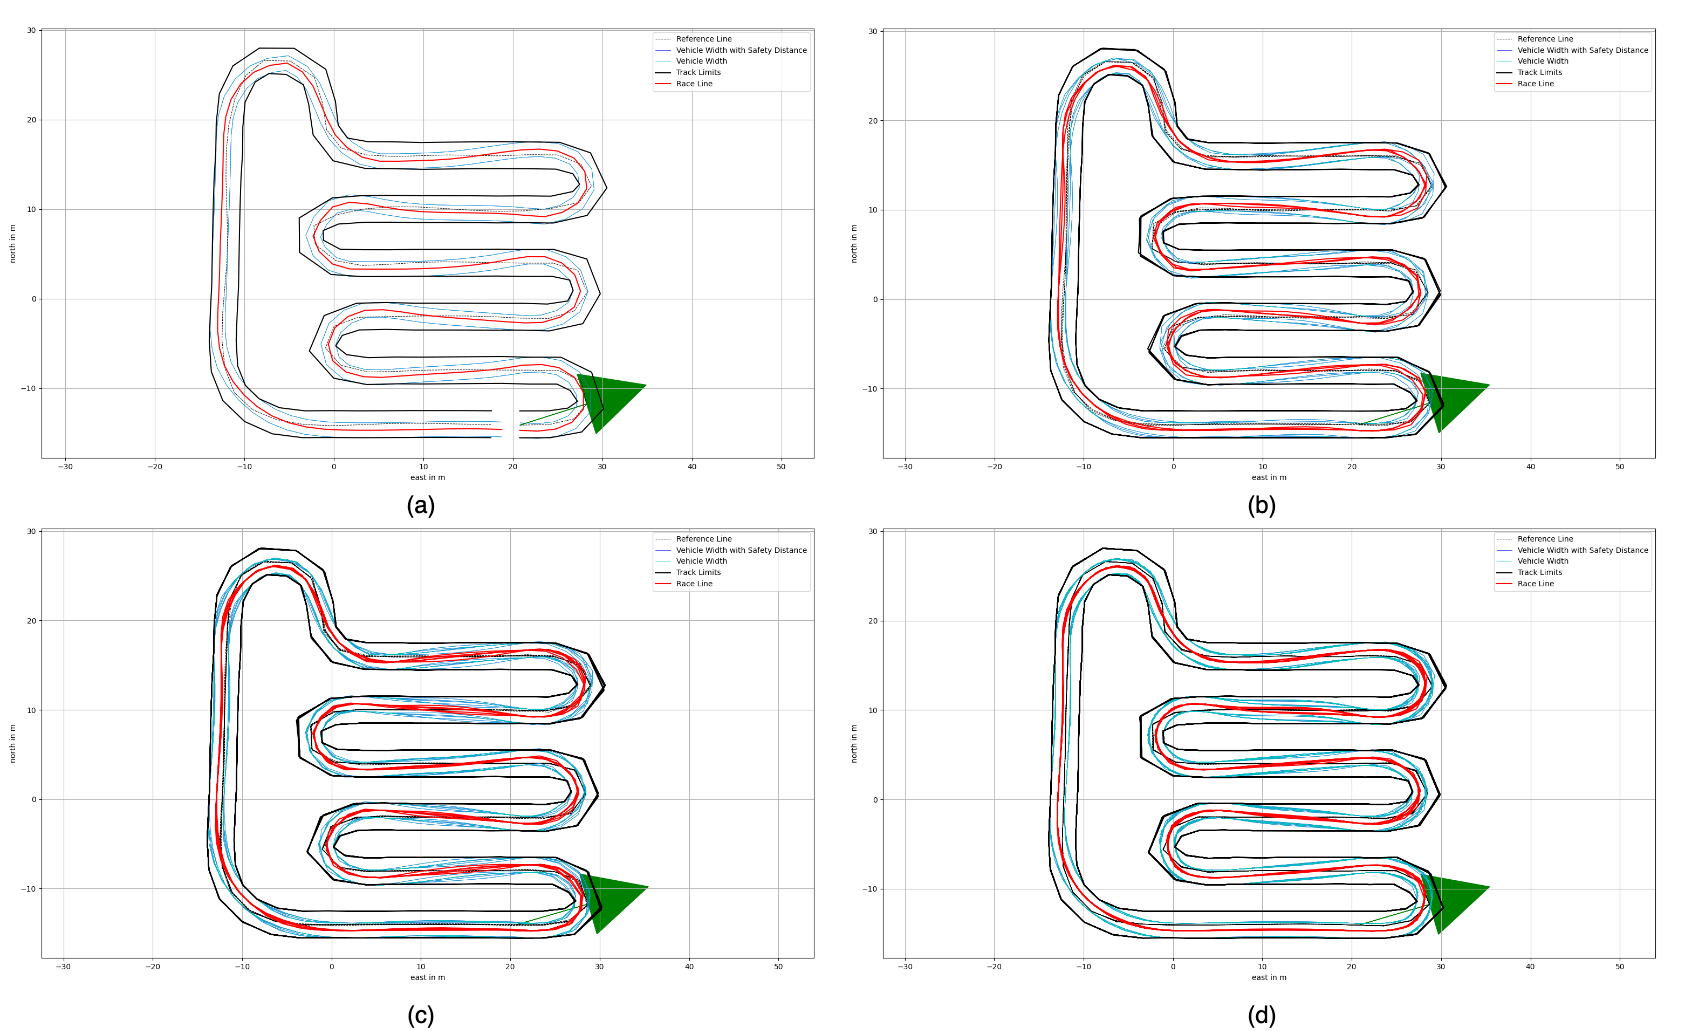
\includegraphics[width=\columnwidth]{Results_Optimization_Comp_2021_Laps_1-8.png}
    \caption{Optimization on the Competition 2021 track with the Minimum Curvature objective for one lap (a), three laps (b), five laps (c), and eight laps (d).}
    \label{fig:Results Comp 2021 Laps 1-8}
\end{figure}

Additionally, the following outputs of the Optimization Algorithm with the Minimum Curvature objective for two laps on the Competition 2021 track are shown: The Velocity and Acceleration Profile in figure \ref{fig:Results Comp 2021 Laps 2 VelAcc Profile}, the Curvature Profile in figure \ref{fig:Results Comp 2021 Laps 2 Curv Profile}, the 3D Velocity Profile in figure \ref{fig:Results Comp 2021 Laps 2 3D Vel Profile}, and the Spline Normals in figure \ref{fig:Results Comp 2021 Laps 2 Spline Normals}.
\begin{figure}[H]
    \centering
    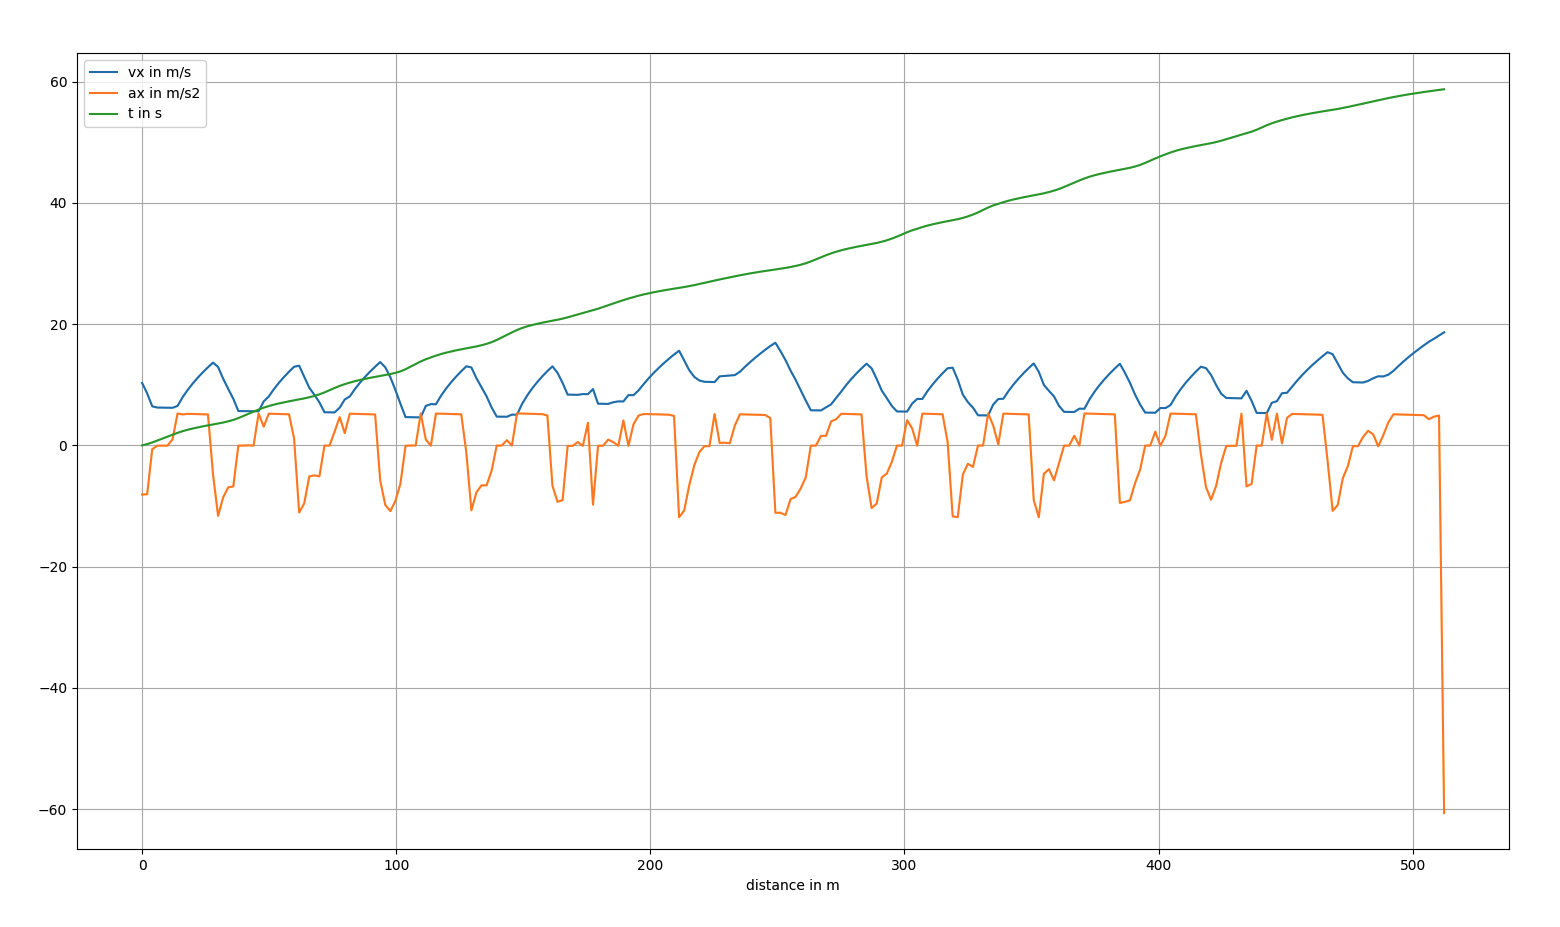
\includegraphics[width=\columnwidth]{Results_Optimization_Comp_2021_Laps_2_VelAcc_Profile.png}
    \caption{The Velocity and Acceleration Profile on the Competition 2021 track for two laps.}
    \label{fig:Results Comp 2021 Laps 2 VelAcc Profile}
\end{figure}
\begin{figure}[H]
    \centering
    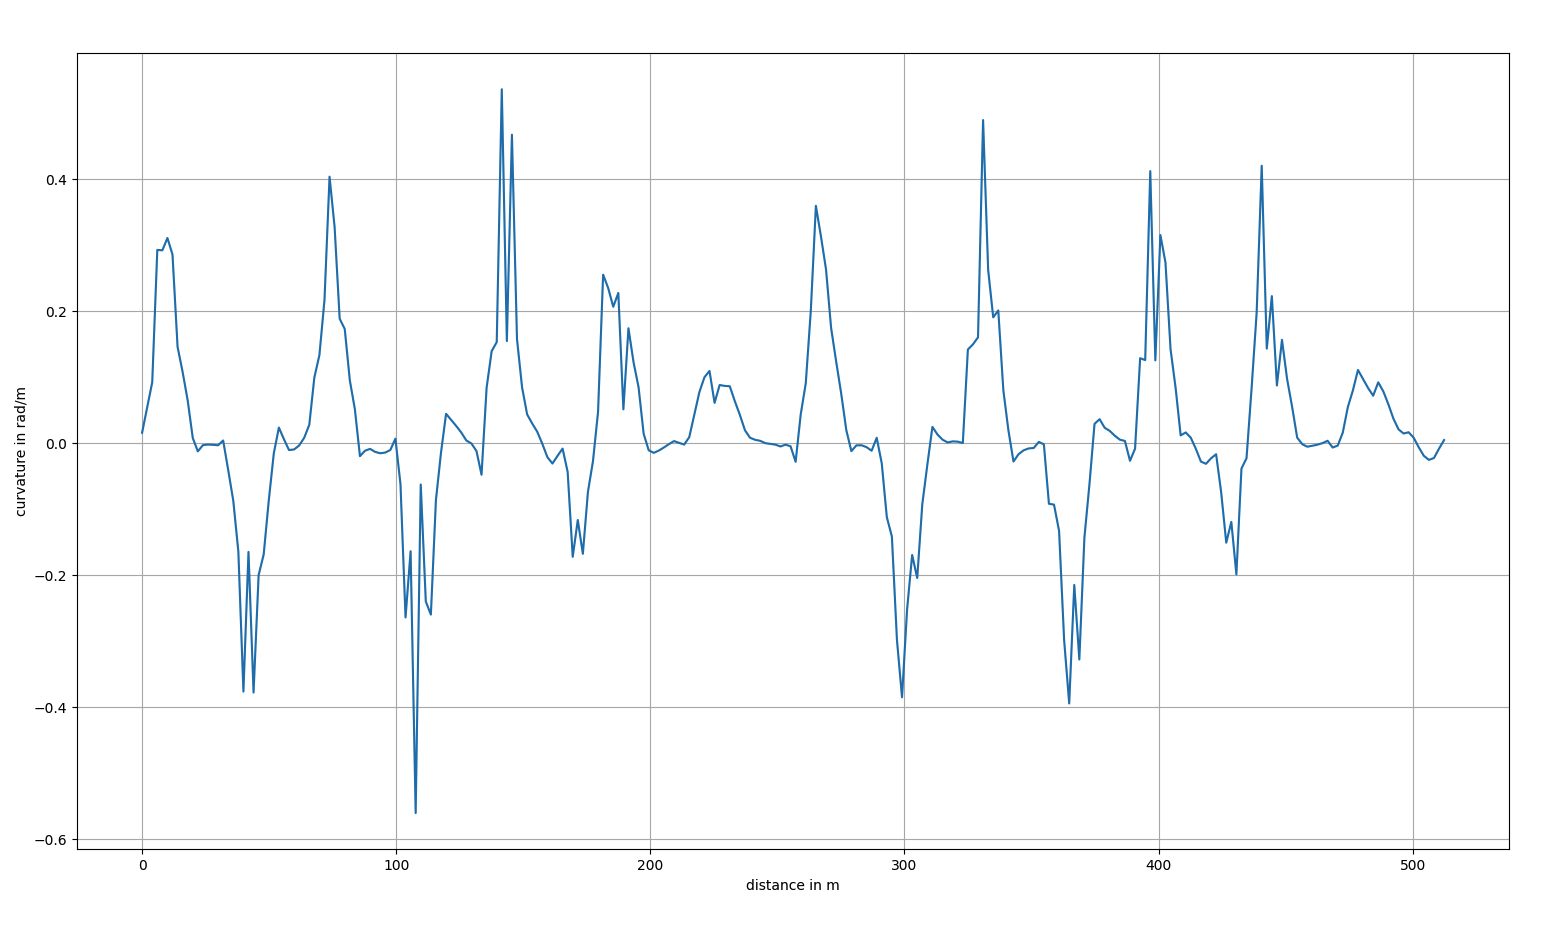
\includegraphics[width=\columnwidth]{Results_Optimization_Comp_2021_Laps_2_Curv_Profile.png}
    \caption{The Curvature Profile on the Competition 2021 track for two laps.}
    \label{fig:Results Comp 2021 Laps 2 Curv Profile}
\end{figure}
\begin{figure}[H]
    \centering
    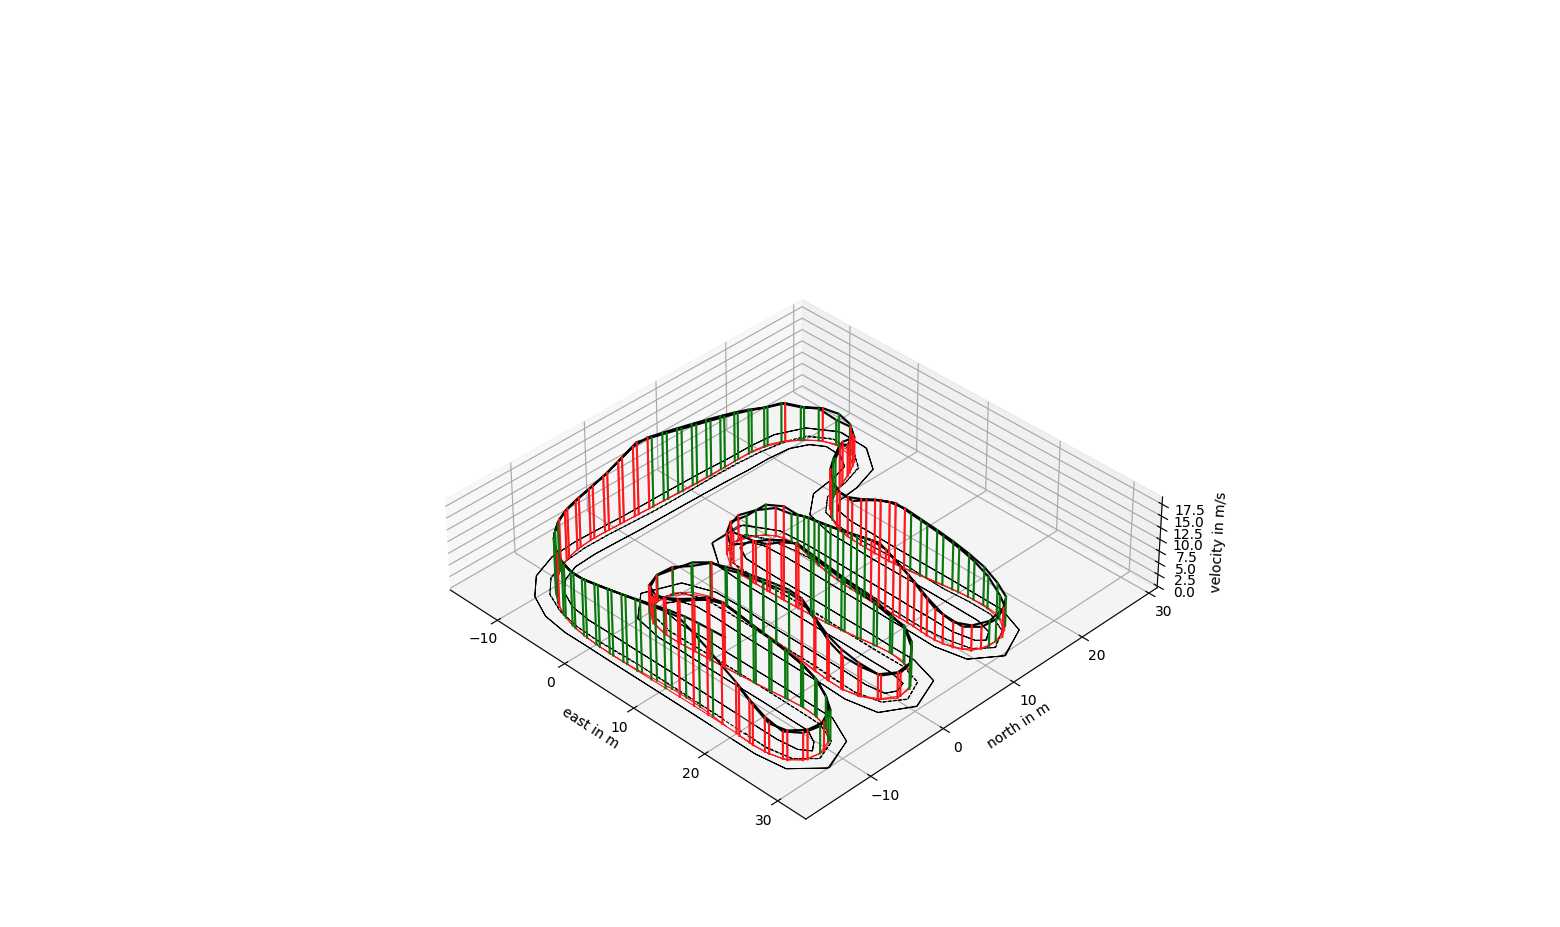
\includegraphics[width=\columnwidth]{Results_Optimization_Comp_2021_Laps_2_3D_Vel_Profile.png}
    \caption{The 3D Velocity Profile on the Competition 2021 track for two laps.}
    \label{fig:Results Comp 2021 Laps 2 3D Vel Profile}
\end{figure}
\begin{figure}[H]
    \centering
    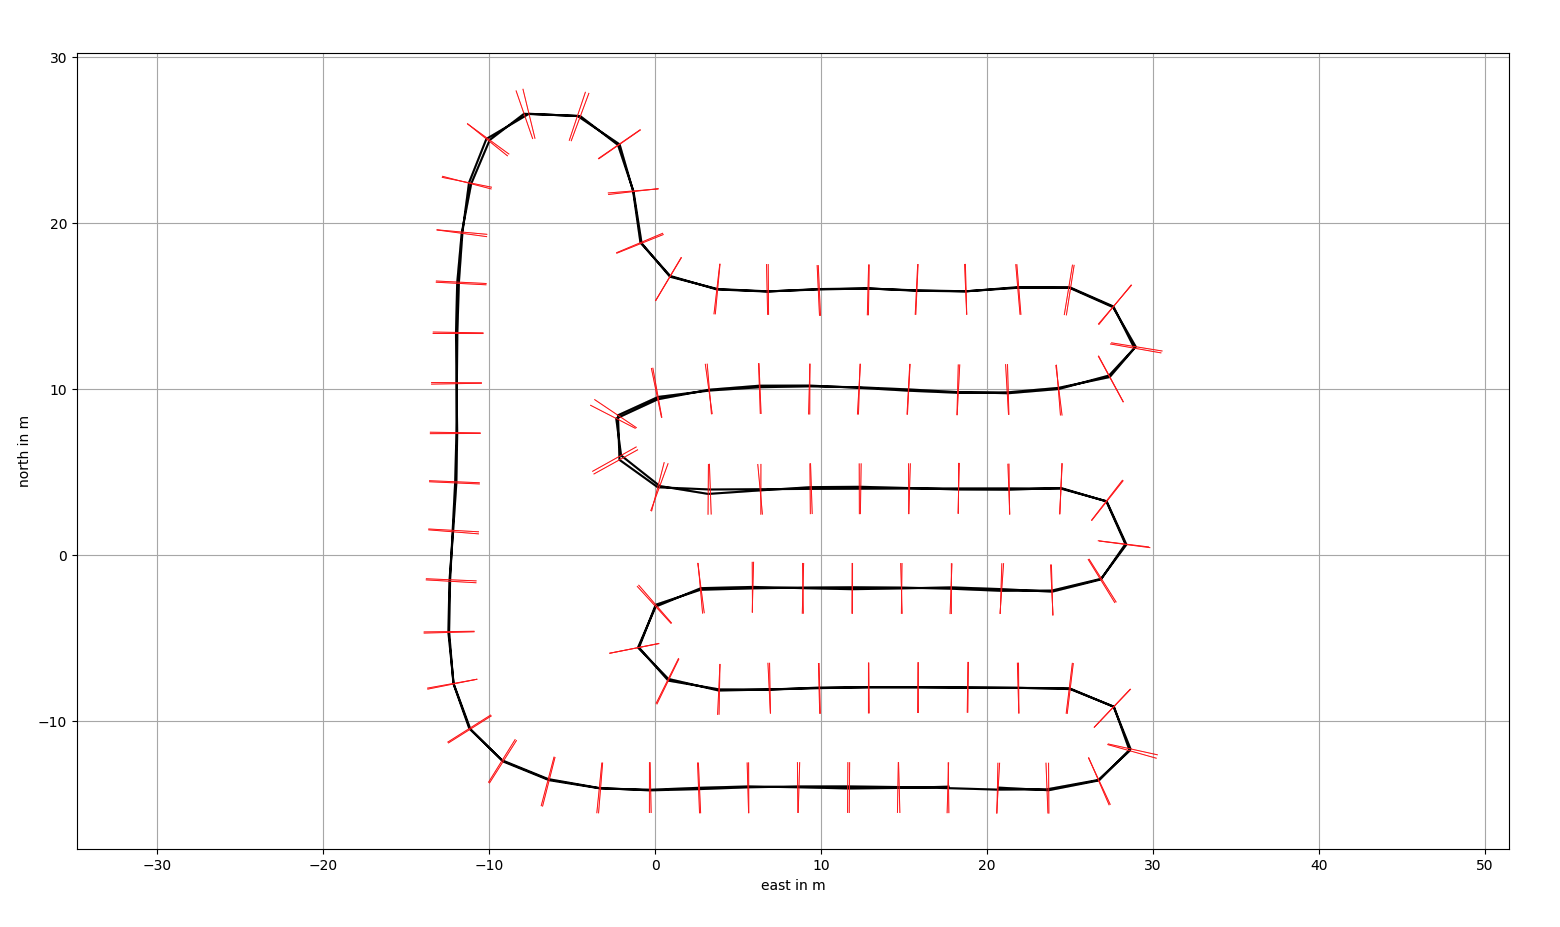
\includegraphics[width=\columnwidth]{Results_Optimization_Comp_2021_Laps_2_Spline_Normals.png}
    \caption{The Spline Normals on the Competition 2021 track for two laps.}
    \label{fig:Results Comp 2021 Laps 2 Spline Normals}
\end{figure}

\section{Garden Light Track} \label{sec:Results Garden Light Track}
An overview of the track is shown in figure \ref{fig:Results Garden Light Initial}. The track was created by the \acrshort{eufs} team too and is called ``Garden Light''. \cite{eufs_sim_gitlab} The track has some parts where the left track limits (blue cones) are very close. Additionally, the track has additional cones on its curves. The track consists of 101 blue cones and 99 yellow cones for the track limits, and 4 big orange cones for the start respectively the end of the track.
\begin{figure}[H]
    \centering
    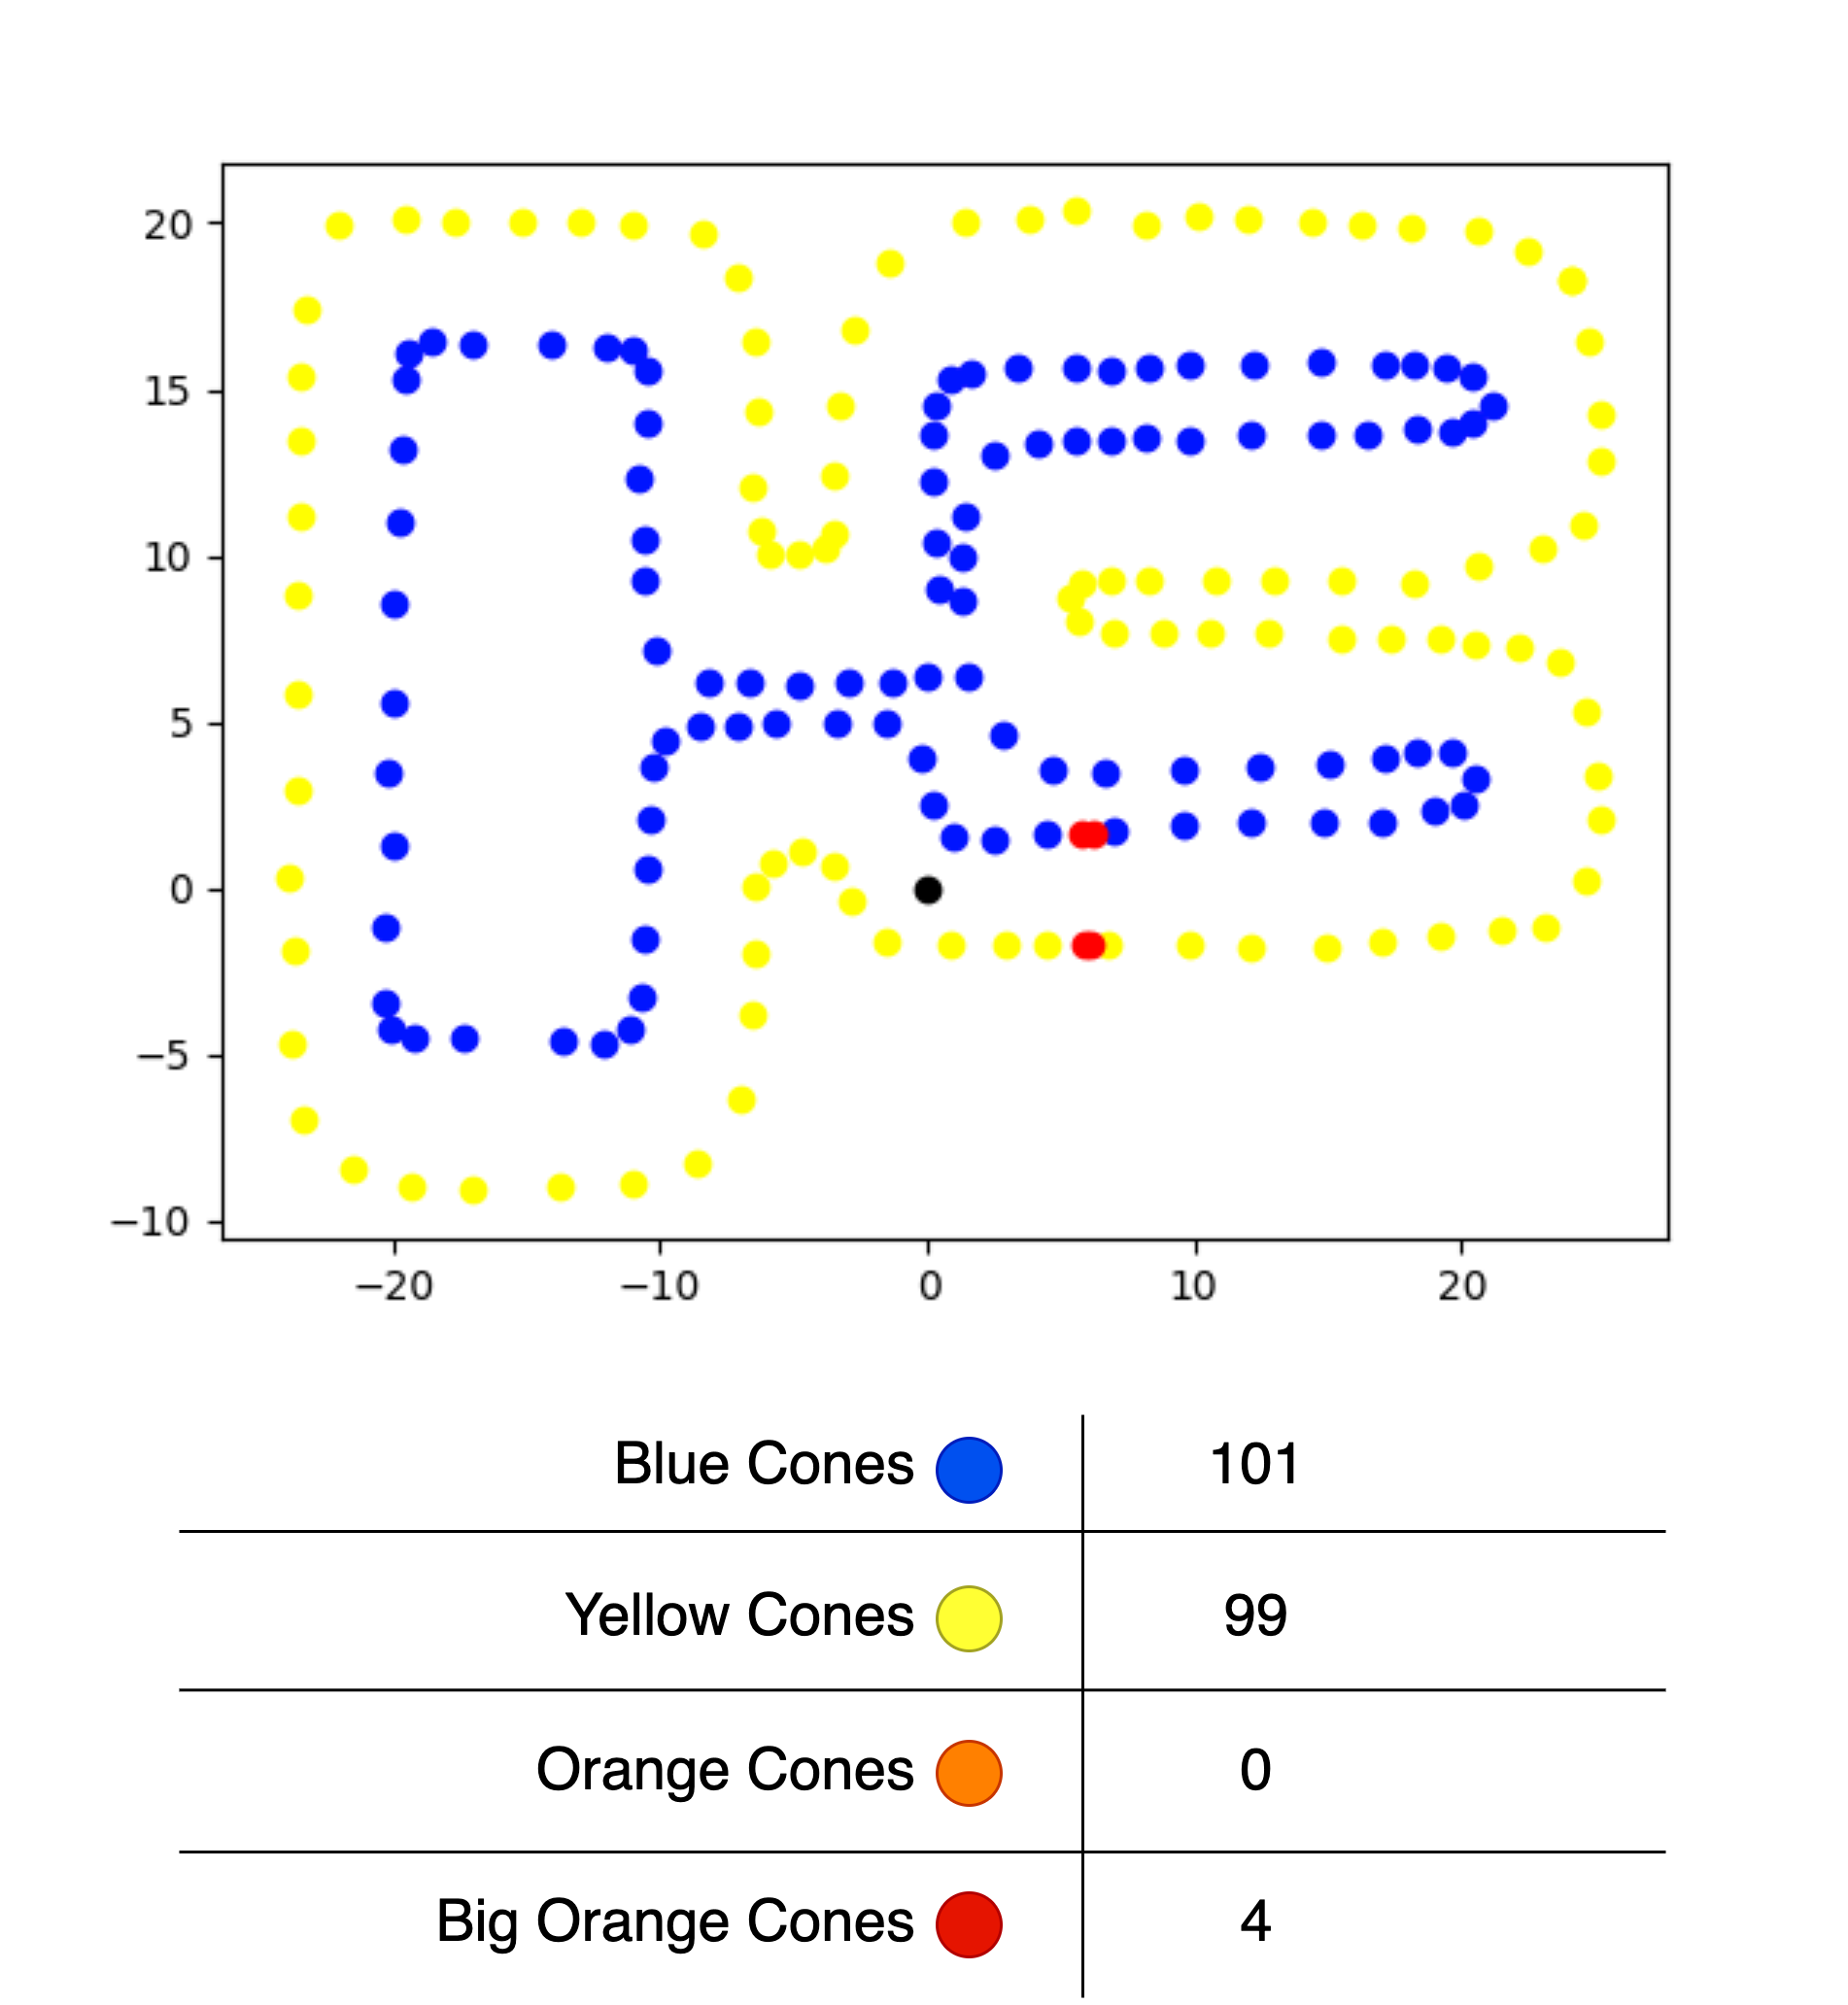
\includegraphics[width=\columnwidth]{Results_Garden_Light_Initial.png}
    \caption{Overview of the Garden Light Track.}
    \label{fig:Results Garden Light Initial}
\end{figure}

\textbf{Exploration Algorithm}

During the run with the Garden Light track, the algorithm did 205 cycles with a total computation time of 0.5926 seconds. The average cycle lasted 0.0029 seconds, with the fastest cycle taking under < 0.0000 seconds long and the slowest cycle taking 0.0076 seconds long. The algorithm created 2631 reference points during the run. The results are listed in table \ref{tab:Results Garden Light Exploration}.

\begin{table}[H]
    \centering
    \begin{tabular}{|l|l|l|}
        \hline
        \textbf{Result}            & \textbf{Value} \\ \hline
        Minimum Cycle Time         & < 0.0000 s     \\ \hline
        Maximum Cycle Time         & 0.0076 s       \\ \hline
        Average Cycle  Time        & 0.0029 s       \\ \hline
        Total Cycle Time           & 0.5926 s       \\ \hline
        Number of Cycles           & 205            \\ \hline
        Generated Reference Points & 2631           \\ \hline
    \end{tabular}
    \caption{Results of the Exploration Algorithm on the Garden Light track.}
    \label{tab:Results Garden Light Exploration}
\end{table}

Figure \ref{fig:Result Garden Light Final} shows the final version of the algorithm on the Garden Light track.
\begin{figure}[H]
    \centering
    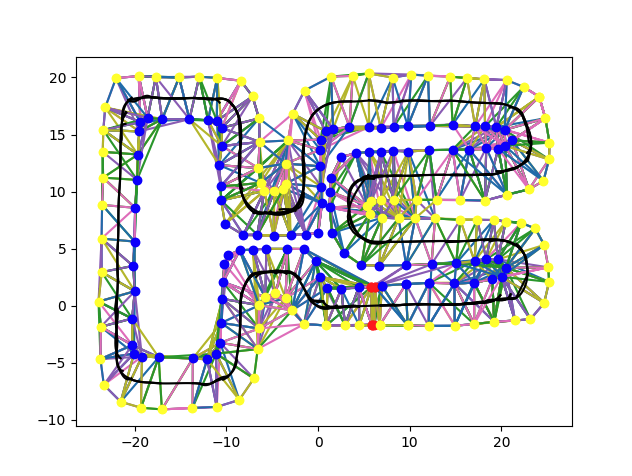
\includegraphics[width=\columnwidth]{Result_GardenLight_final.png}
    \caption{The Garden Light track with the final algorithm implementation.}
    \label{fig:Result Garden Light Final}
\end{figure}

\textbf{Optimization Algorithm}

A comparison of the different objectives on the Garden Light track is given in table \ref{tab:Results Garden Light Optimization Objectives}. Two laps on the given track were calculated for each objective: Shortest Path, Minimum Curvature and Minimum Curvature with iterative call. The result with the Shortest Path objective is seen in figure \ref{fig:Results Garden Light Laps 2 Shortest Path}, the result with the Minimum Curvature objective is seen in figure \ref{fig:Results Garden Light Laps 2 Minimum Curvature}, and the calculation with the Minimum Curvature objective with an iterative call did not finish in a reasonable time.

\begin{table}[H]
    \centering
    \begin{tabular}{|l|l|l|l|}
        \hline
        \textbf{Objective}    & \textbf{Runtime} & \textbf{Estimated Lap Time} & \textbf{Generated Reference Points} \\ \hline
        Shortest Path         & 0.15 s           & 47.39 s                     & 159 Reference Points                \\ \hline
        Minimum Curvature     & 0.17 s           & 48.72 s                     & 173 Reference Points                \\ \hline
        Minimum Curvature IQP & DNF*             & DNF*                        & DNF*                                \\ \hline
    \end{tabular}
    \caption{Results of the different Optimization Algorithm objectives on the Garden Light track for two laps. (* Did not finish)}
    \label{tab:Results Garden Light Optimization Objectives}
\end{table}
\begin{figure}[H]
    \centering
    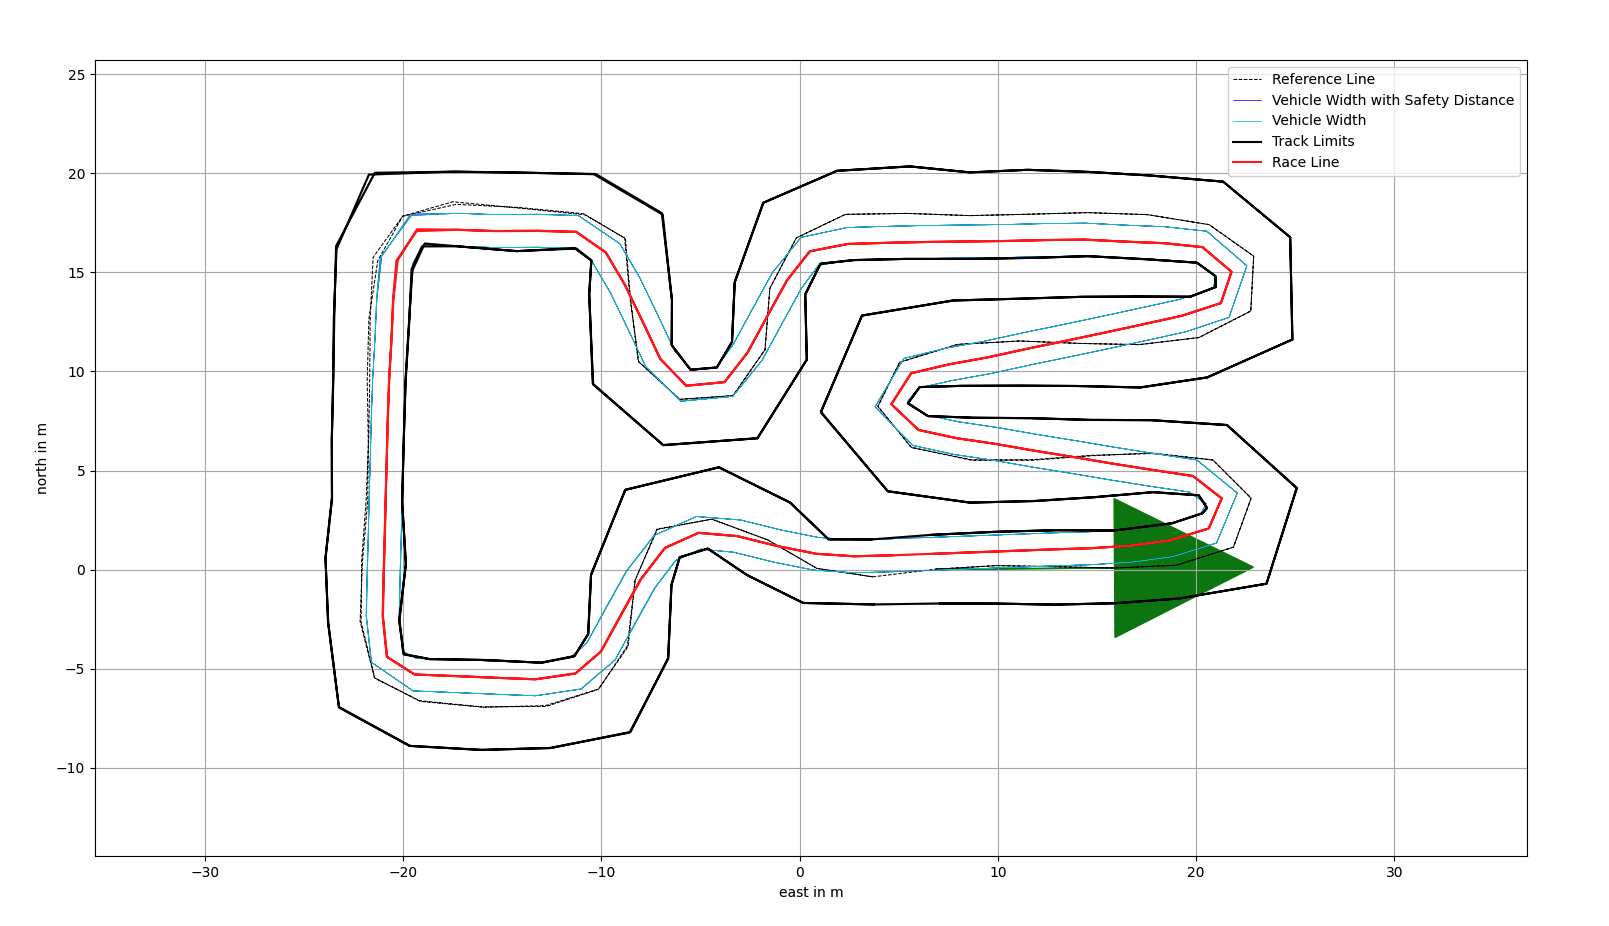
\includegraphics[width=\columnwidth]{Results_Optimization_Garden_Light_Laps_2_Shortest_Path.png}
    \caption{Optimization on the Garden Light track for two laps with the Shortest Path objective.}
    \label{fig:Results Garden Light Laps 2 Shortest Path}
\end{figure}
\begin{figure}[H]
    \centering
    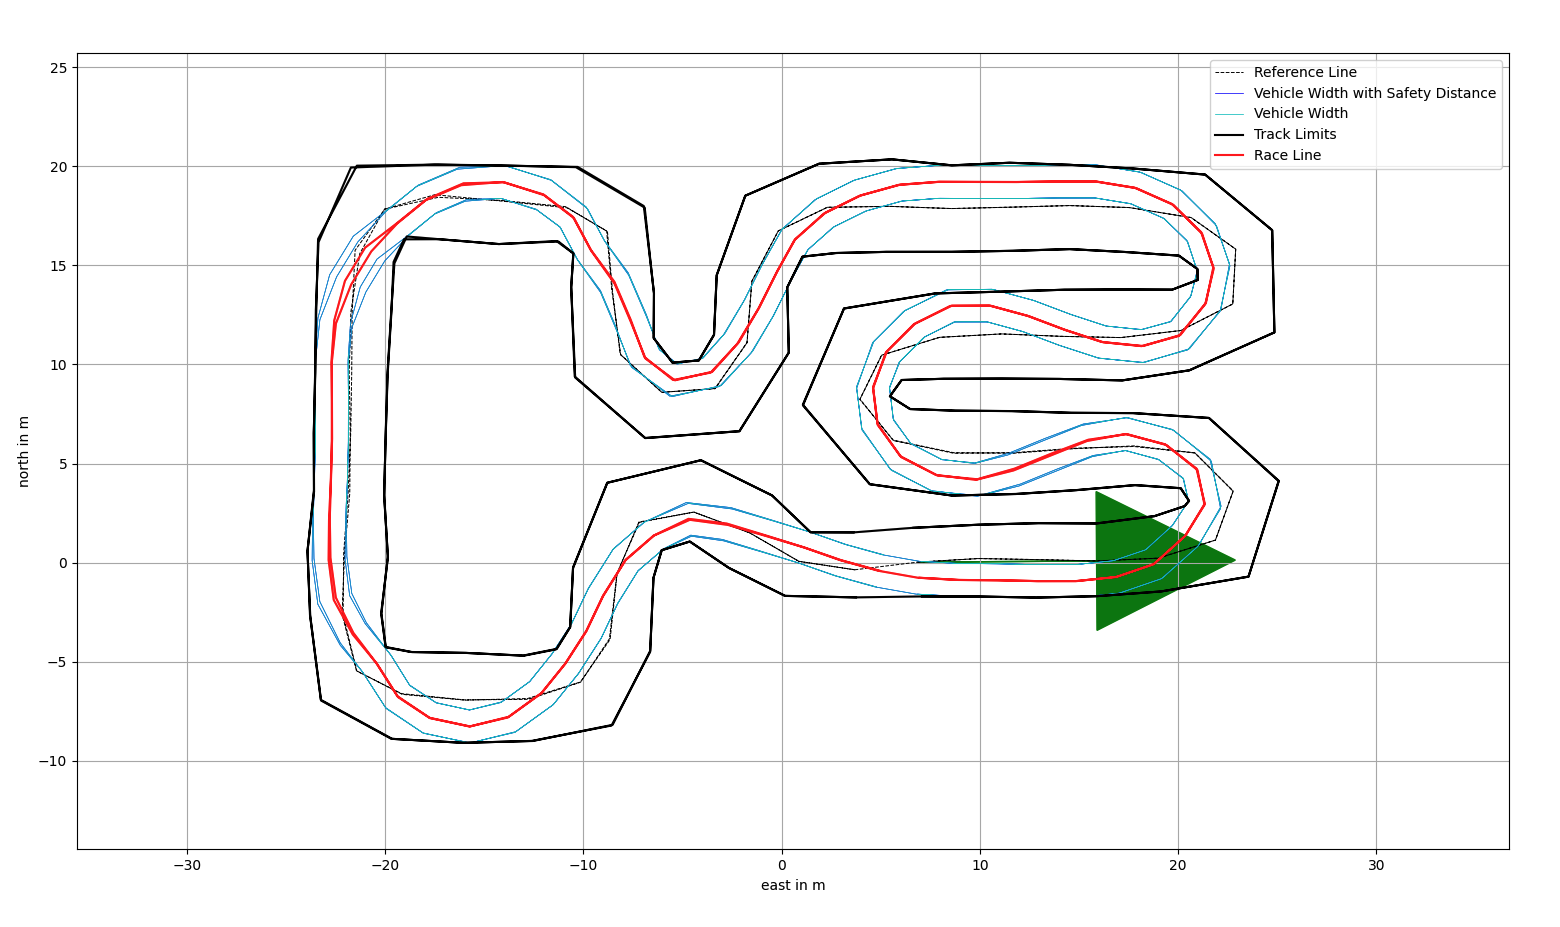
\includegraphics[width=\columnwidth]{Results_Optimization_Garden_Light_Laps_2.png}
    \caption{Optimization on the Garden Light track for two laps with the Minimum Curvature objective.}
    \label{fig:Results Garden Light Laps 2 Minimum Curvature}
\end{figure}

The results for the Optimization Algorithm with the Minimum Curvature objective for one lap, two laps, three laps, five laps and eight laps are detailed in table \ref{tab:Results Garden Light Optimization Laps 1-8}. The visual comparison of the output between one lap, three laps, five laps and eight laps is shown in figure \ref{fig:Results Garden Light Laps 1-8}.

\begin{table}[H]
    \centering
    \begin{tabular}{|l|l|l|l|}
        \hline
        \textbf{Laps} & \textbf{Runtime} & \textbf{Estimated Lap Time} & \textbf{Generated Reference Points} \\ \hline
        1             & 0.07 s           & 25.20 s                     & 88 Reference Points                 \\ \hline
        2             & 0.17 s           & 48.72 s                     & 173 Reference Points                \\ \hline
        3             & 0.29 s           & 71.59 s                     & 258 Reference Points                \\ \hline
        5             & 0.74 s           & 117.31 s                    & 428 Reference Points                \\ \hline
        8             & 2.03 s           & 190.31 s                    & 682 Reference Points                \\ \hline
    \end{tabular}
    \caption{Results of the Optimization Algorithm with the Minimum Curvature objective on the Garden Light track for one to eight laps.}
    \label{tab:Results Garden Light Optimization Laps 1-8}
\end{table}
\begin{figure}[H]
    \centering
    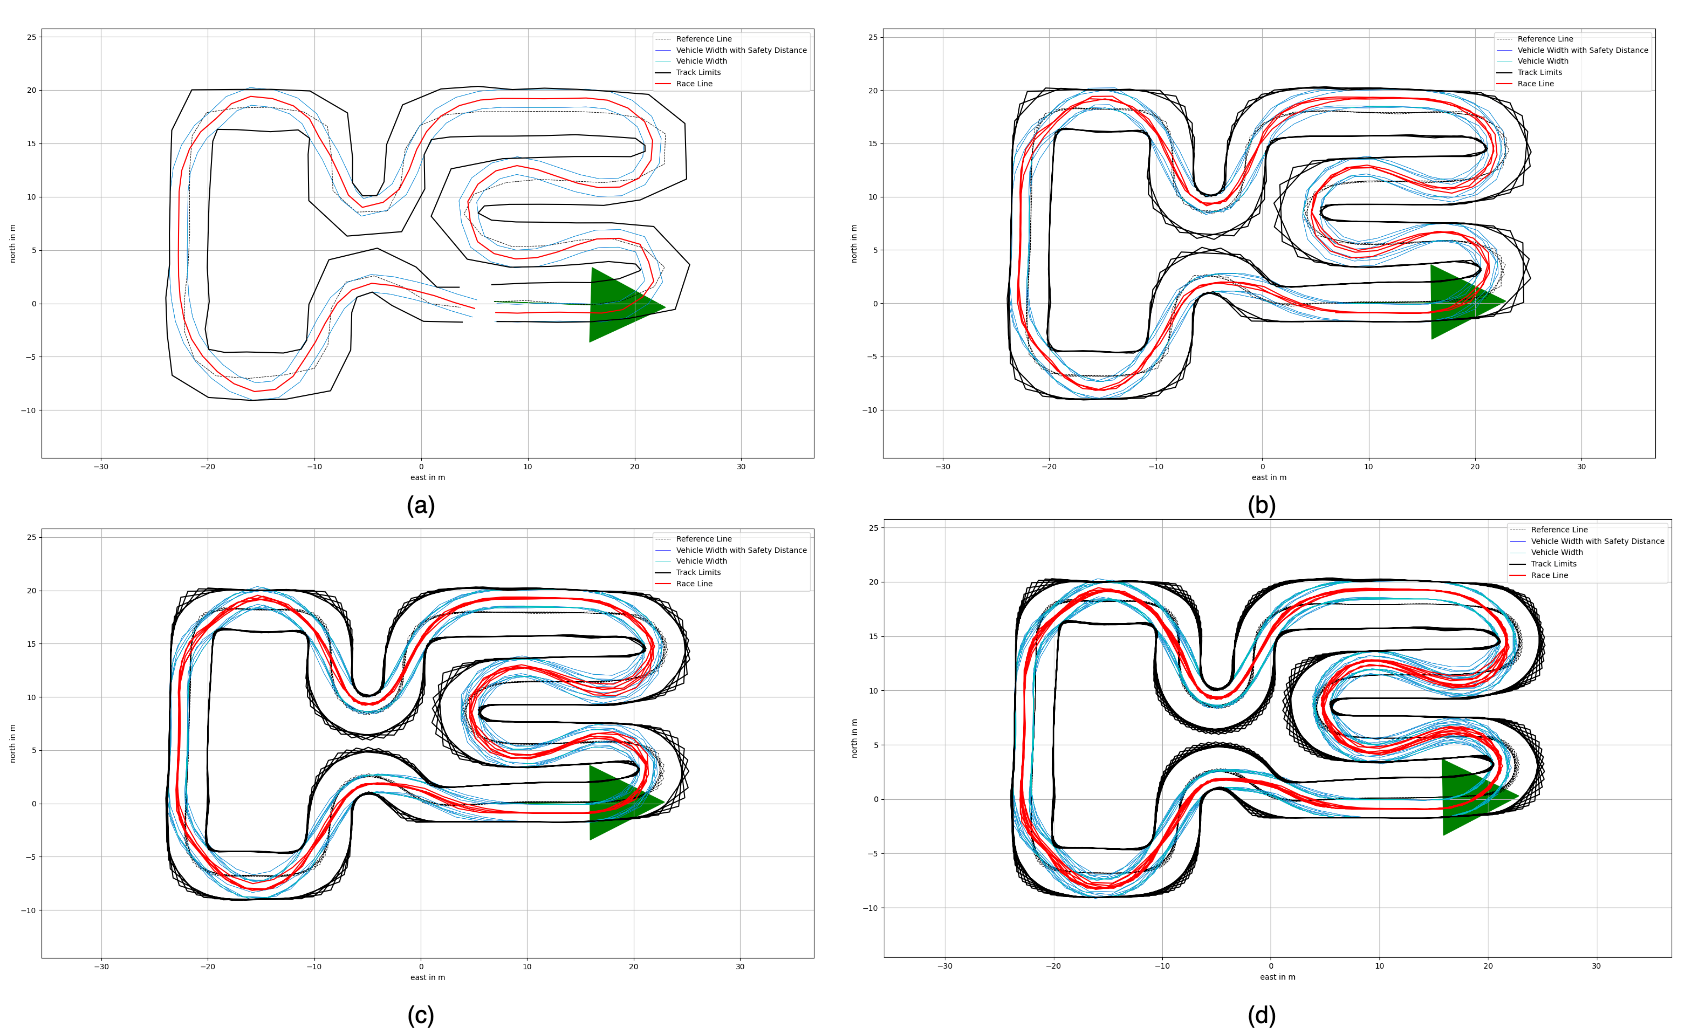
\includegraphics[width=\columnwidth]{Results_Optimization_Garden_Light_Laps_1-8.png}
    \caption{Optimization on the Garden Light track with the Minimum Curvature objective for one lap (a), three laps (b), five laps (c), and eight laps (d).}
    \label{fig:Results Garden Light Laps 1-8}
\end{figure}

Additionally, the following outputs of the Optimization Algorithm with the Minimum Curvature objective for two laps on the Garden Light track are shown: The Velocity and Acceleration Profile in figure \ref{fig:Results Garden Light Laps 2 VelAcc Profile}, the Curvature Profile in figure \ref{fig:Results Garden Light Laps 2 Curv Profile}, the 3D Velocity Profile in figure \ref{fig:Results Garden Light Laps 2 3D Vel Profile}, and the Spline Normals in figure \ref{fig:Results Garden Light Laps 2 Spline Normals}.
\begin{figure}[H]
    \centering
    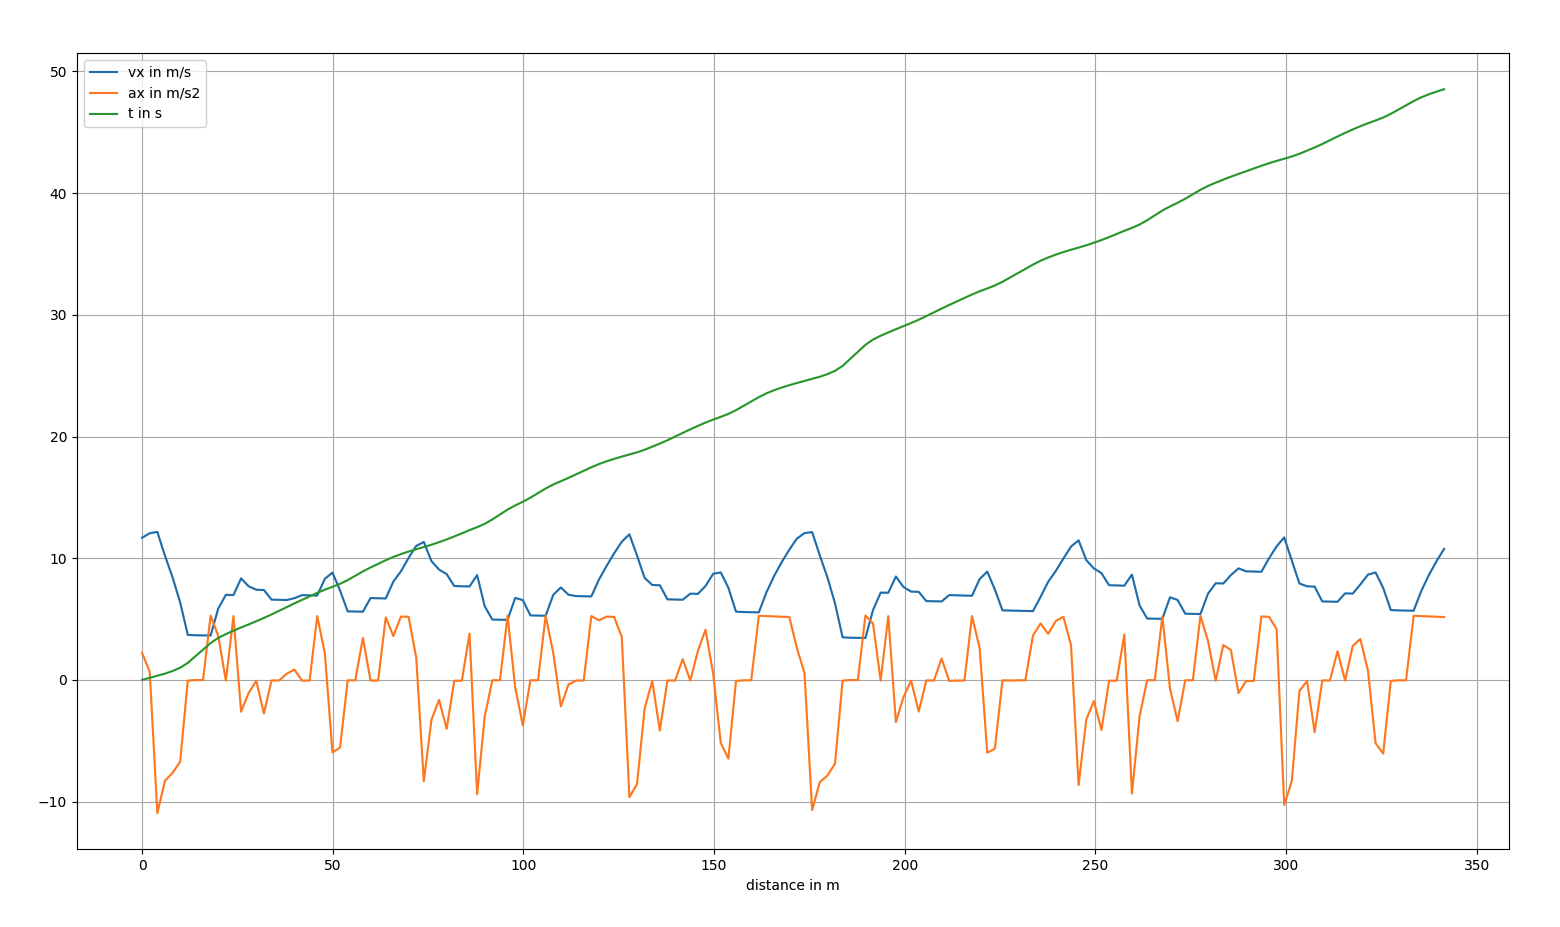
\includegraphics[width=\columnwidth]{Results_Optimization_Garden_Light_Laps_2_VelAcc_Profile.png}
    \caption{The Velocity and Acceleration Profile on the Garden Light track for two laps.}
    \label{fig:Results Garden Light Laps 2 VelAcc Profile}
\end{figure}
\begin{figure}[H]
    \centering
    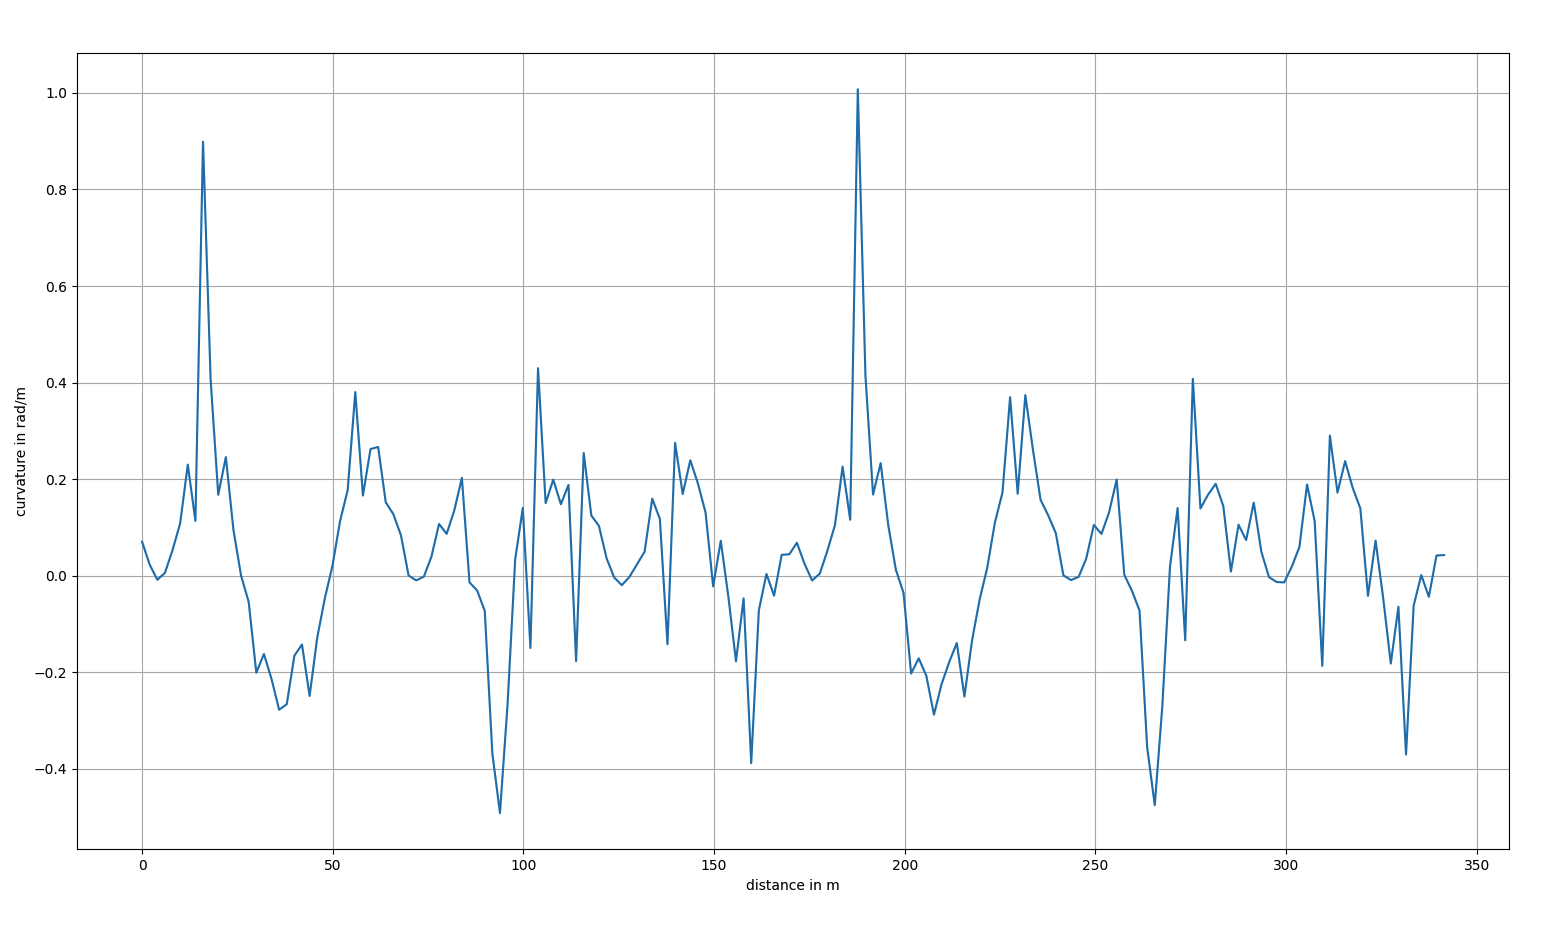
\includegraphics[width=\columnwidth]{Results_Optimization_Garden_Light_Laps_2_Curv_Profile.png}
    \caption{The Curvature Profile on the Garden Light track for two laps.}
    \label{fig:Results Garden Light Laps 2 Curv Profile}
\end{figure}
\begin{figure}[H]
    \centering
    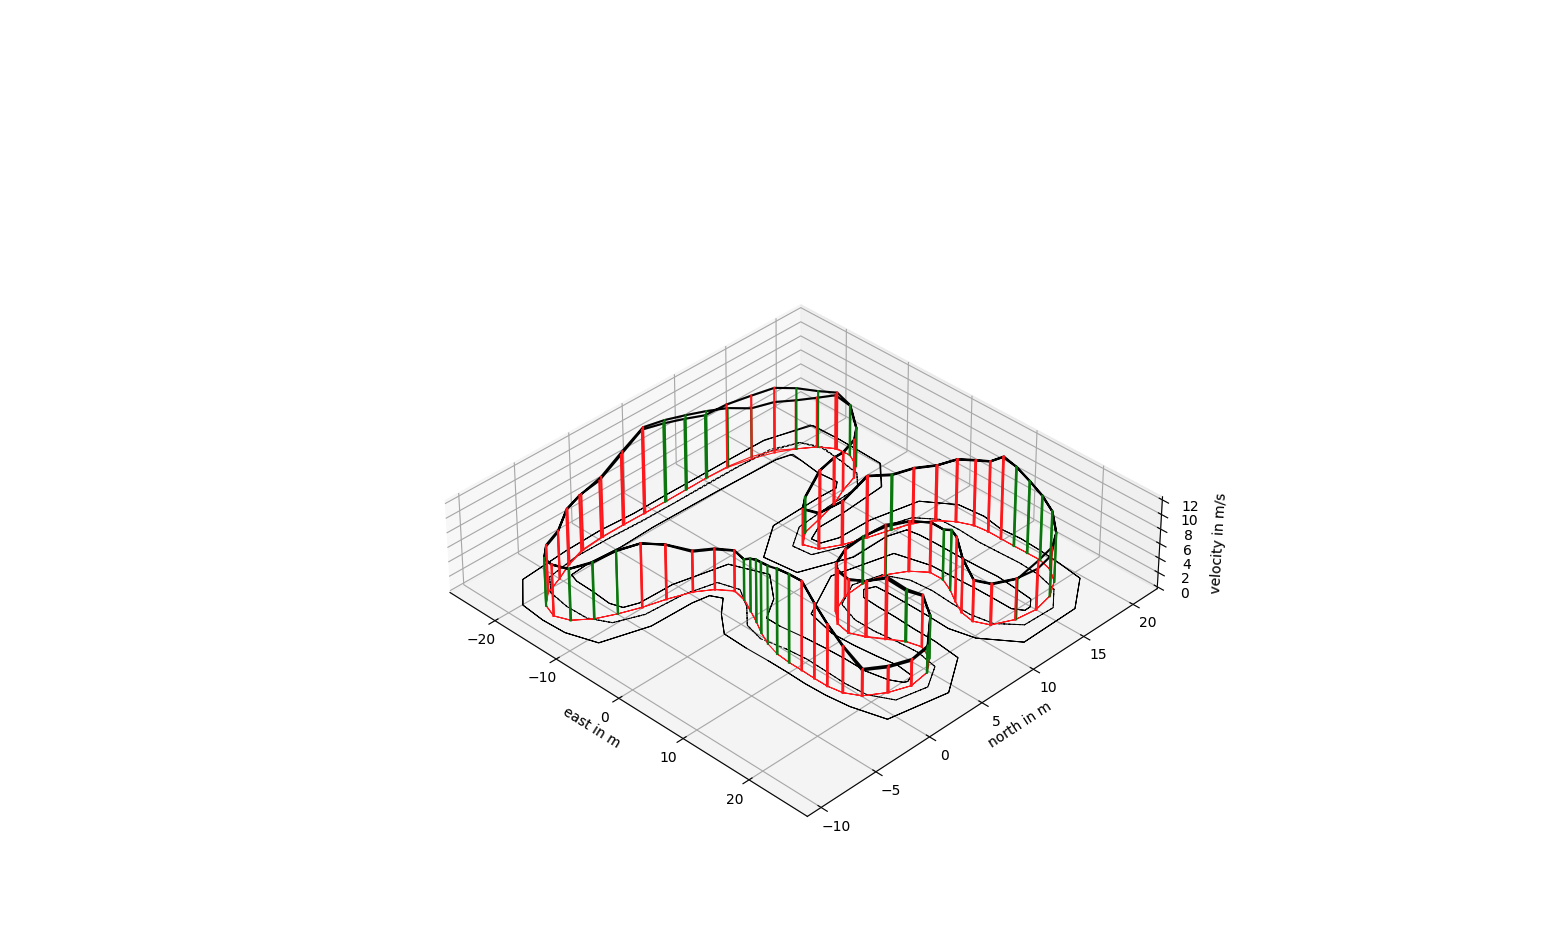
\includegraphics[width=\columnwidth]{Results_Optimization_Garden_Light_Laps_2_3D_Vel_Profile.png}
    \caption{The 3D Velocity Profile on the Garden Light track for two laps.}
    \label{fig:Results Garden Light Laps 2 3D Vel Profile}
\end{figure}
\begin{figure}[H]
    \centering
    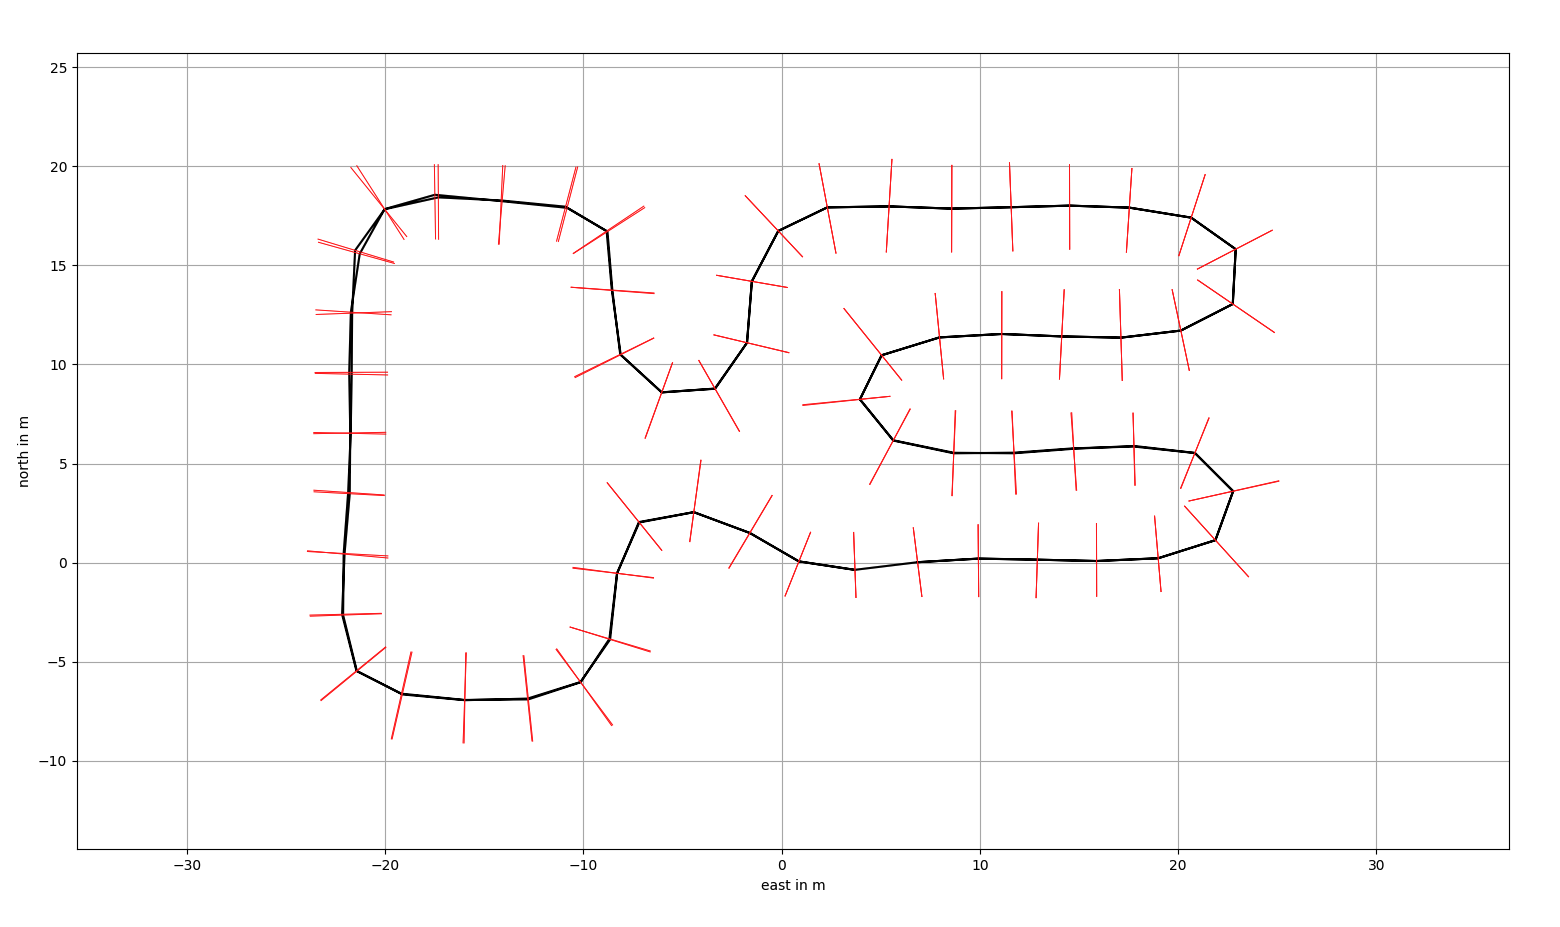
\includegraphics[width=\columnwidth]{Results_Optimization_Garden_Light_Laps_2_Spline_Normals.png}
    \caption{The Spline Normals on the Garden Light track for two laps.}
    \label{fig:Results Garden Light Laps 2 Spline Normals}
\end{figure}

\section{Rounded Rectangle Track} \label{sec:Results Rounded Rectangle Track}
The track was created by \acrshort{tumftm} and was provided together with the ``global\_racetrajectory\_optimization'' repository. \cite{tumftm_optimization_algoritm}
As the track information came already in the format which would be generated by the 'Optimization Input Transformer' described in section \ref{sec:Optimization Input Transformer}, the track could only be tested with the Optimization Algorithm, but not with the Exploration Algorithm.

\textbf{Optimization Algorithm}

A comparison of the different objectives on the Rounded Rectangle track is given in table \ref{tab:Results Rounded Rectangle Optimization Objectives}. Two laps on the given track were calculated for each objective: Shortest Path, Minimum Curvature and Minimum Curvature with iterative call. The result with the Shortest Path objective is seen in figure \ref{fig:Results Rounded Rectangle Laps 2 Shortest Path}, the result with the Minimum Curvature objective is seen in figure \ref{fig:Results Rounded Rectangle Laps 2 Minimum Curvature}, and the result with the Minimum Curvature objective with an iterative call is seen in figure \ref{fig:Results Rounded Rectangle Laps 2 Minimum Curvature IQP}.

\begin{table}[H]
    \centering
    \begin{tabular}{|l|l|l|l|}
        \hline
        \textbf{Objective}    & \textbf{Runtime} & \textbf{Estimated Lap Time} & \textbf{Generated Reference Points} \\ \hline
        Shortest Path         & 0.32 s           & 38.39 s                     & 293 Reference Points                \\ \hline
        Minimum Curvature     & 0.39 s           & 36.18 s                     & 310 Reference Points                \\ \hline
        Minimum Curvature IQP & 0.59 s           & 31.28 s                     & 303 Reference Points                \\ \hline
    \end{tabular}
    \caption{Results of the different Optimization Algorithm objectives on the Rounded Rectangle track for two laps.}
    \label{tab:Results Rounded Rectangle Optimization Objectives}
\end{table}
\begin{figure}[H]
    \centering
    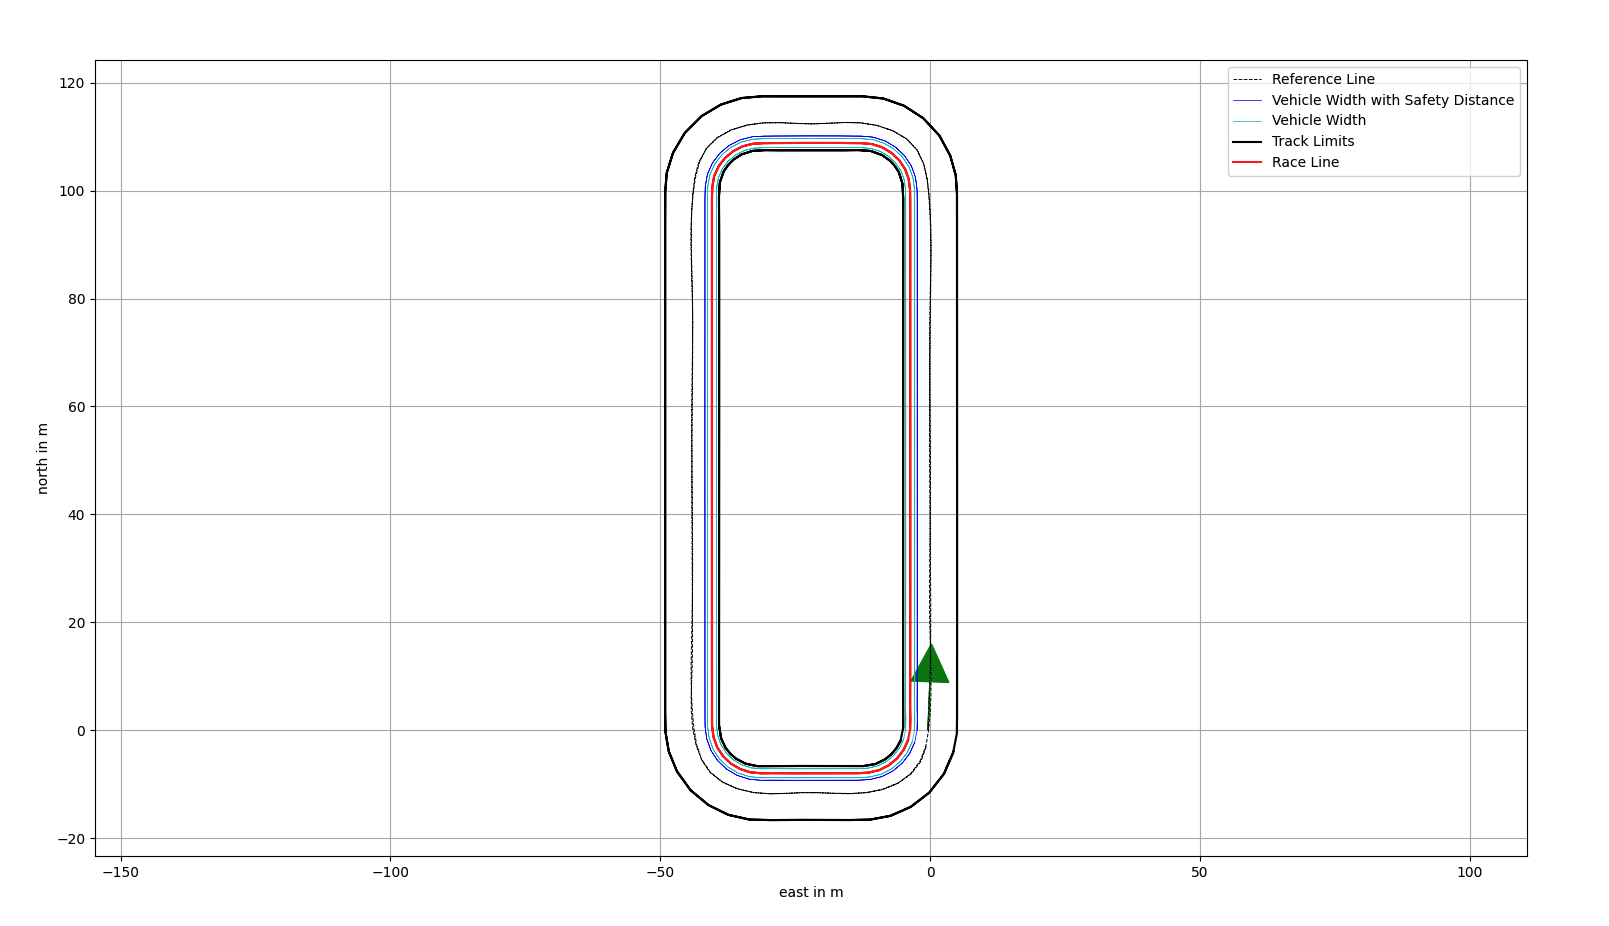
\includegraphics[width=\columnwidth]{Results_Optimization_Rounded_Rectangle_Laps_2_Shortest_Path.png}
    \caption{Optimization on the Rounded Rectangle track for two laps with the Shortest Path objective.}
    \label{fig:Results Rounded Rectangle Laps 2 Shortest Path}
\end{figure}
\begin{figure}[H]
    \centering
    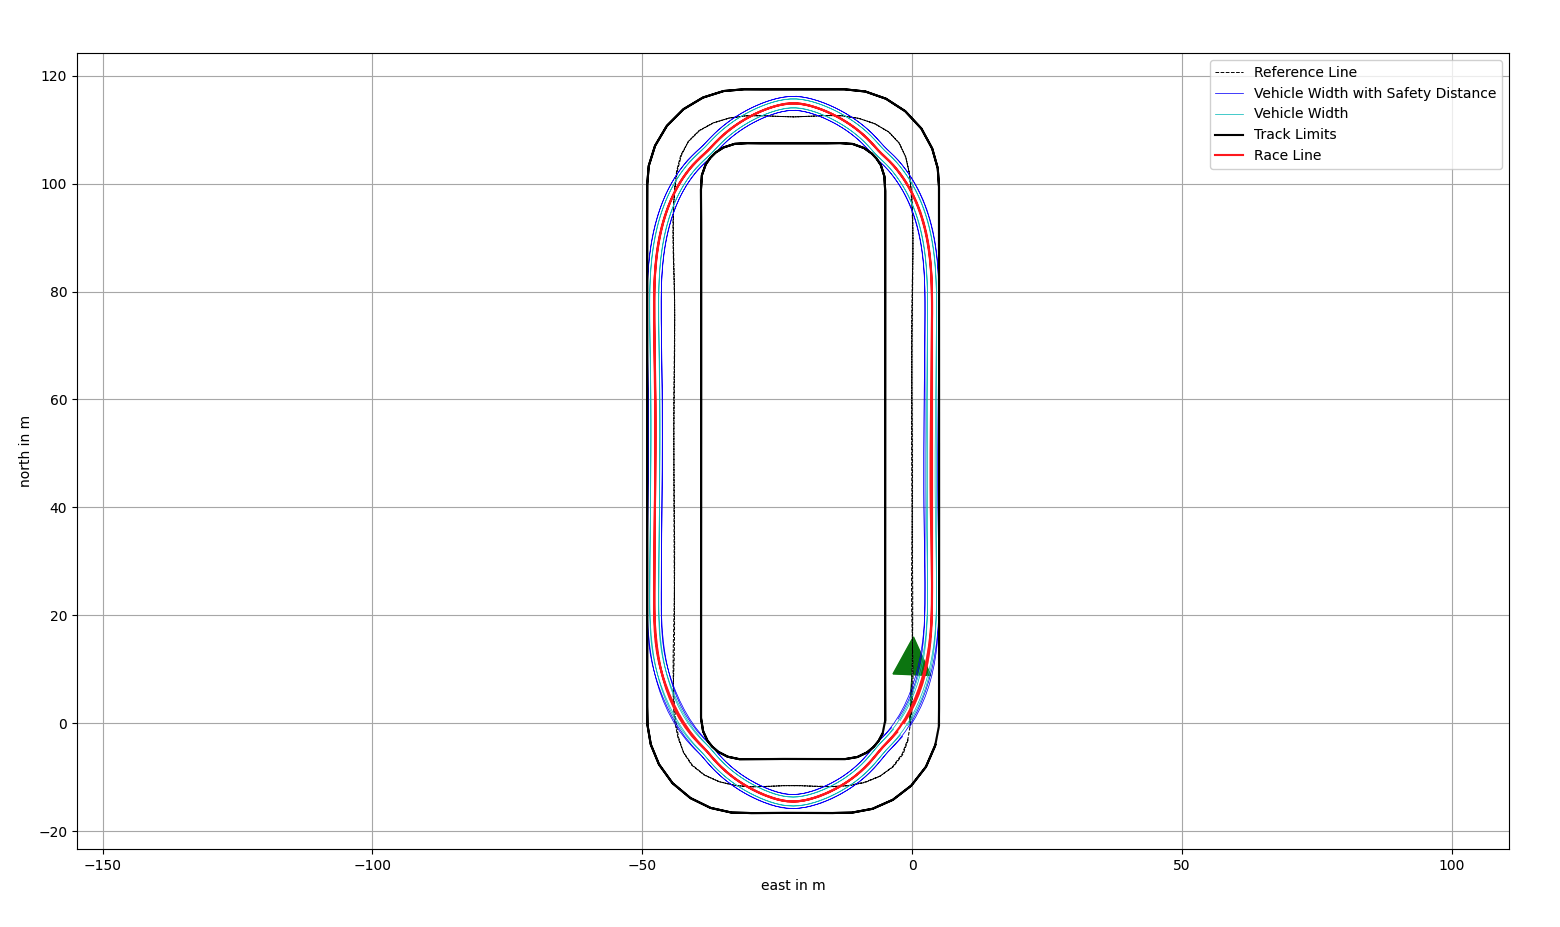
\includegraphics[width=\columnwidth]{Results_Optimization_Rounded_Rectangle_Laps_2.png}
    \caption{Optimization on the Rounded Rectangle track for two laps with the Minimum Curvature objective.}
    \label{fig:Results Rounded Rectangle Laps 2 Minimum Curvature}
\end{figure}
\begin{figure}[H]
    \centering
    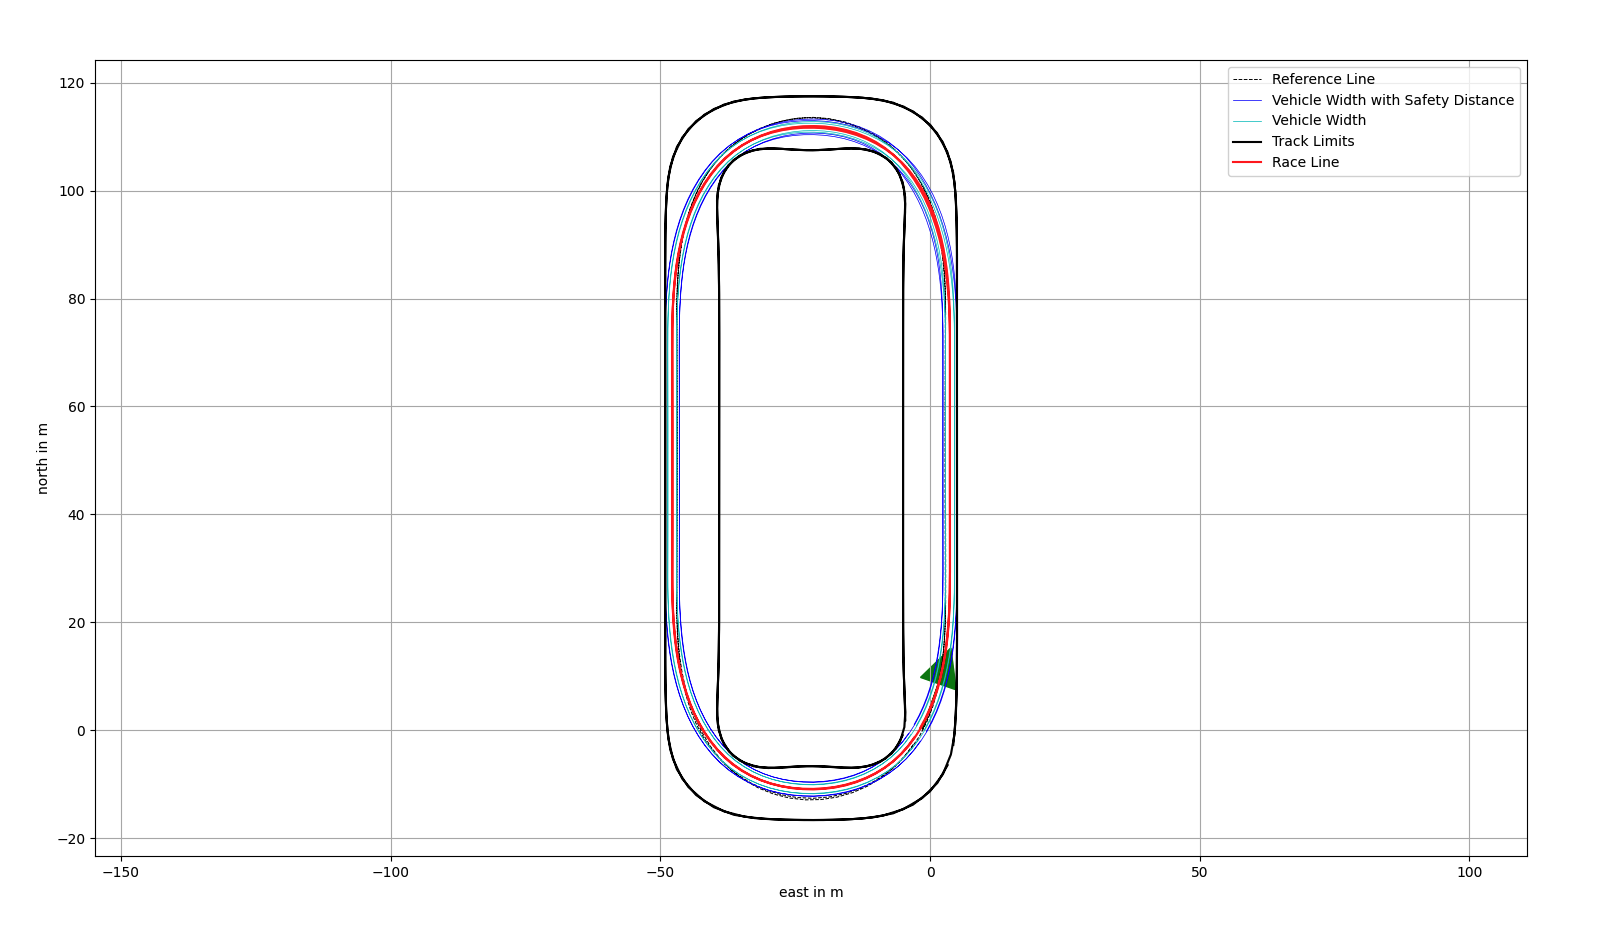
\includegraphics[width=\columnwidth]{Results_Optimization_Rounded_Rectangle_Laps_2_Mincurv_IQP.png}
    \caption{Optimization on the Rounded Rectangle track for two laps with the Minimum Curvature objective with iterative call.}
    \label{fig:Results Rounded Rectangle Laps 2 Minimum Curvature IQP}
\end{figure}

Additionally, the following outputs of the Optimization Algorithm with the Minimum Curvature objective for two laps on the Rounded Rectangle track are shown: The Velocity and Acceleration Profile in figure \ref{fig:Results Rounded Rectangle Laps 2 VelAcc Profile}, the Curvature Profile in figure \ref{fig:Results Rounded Rectangle Laps 2 Curv Profile}, and the Spline Normals in figure \ref{fig:Results Rounded Rectangle Laps 2 Spline Normals}.
\begin{figure}[H]
    \centering
    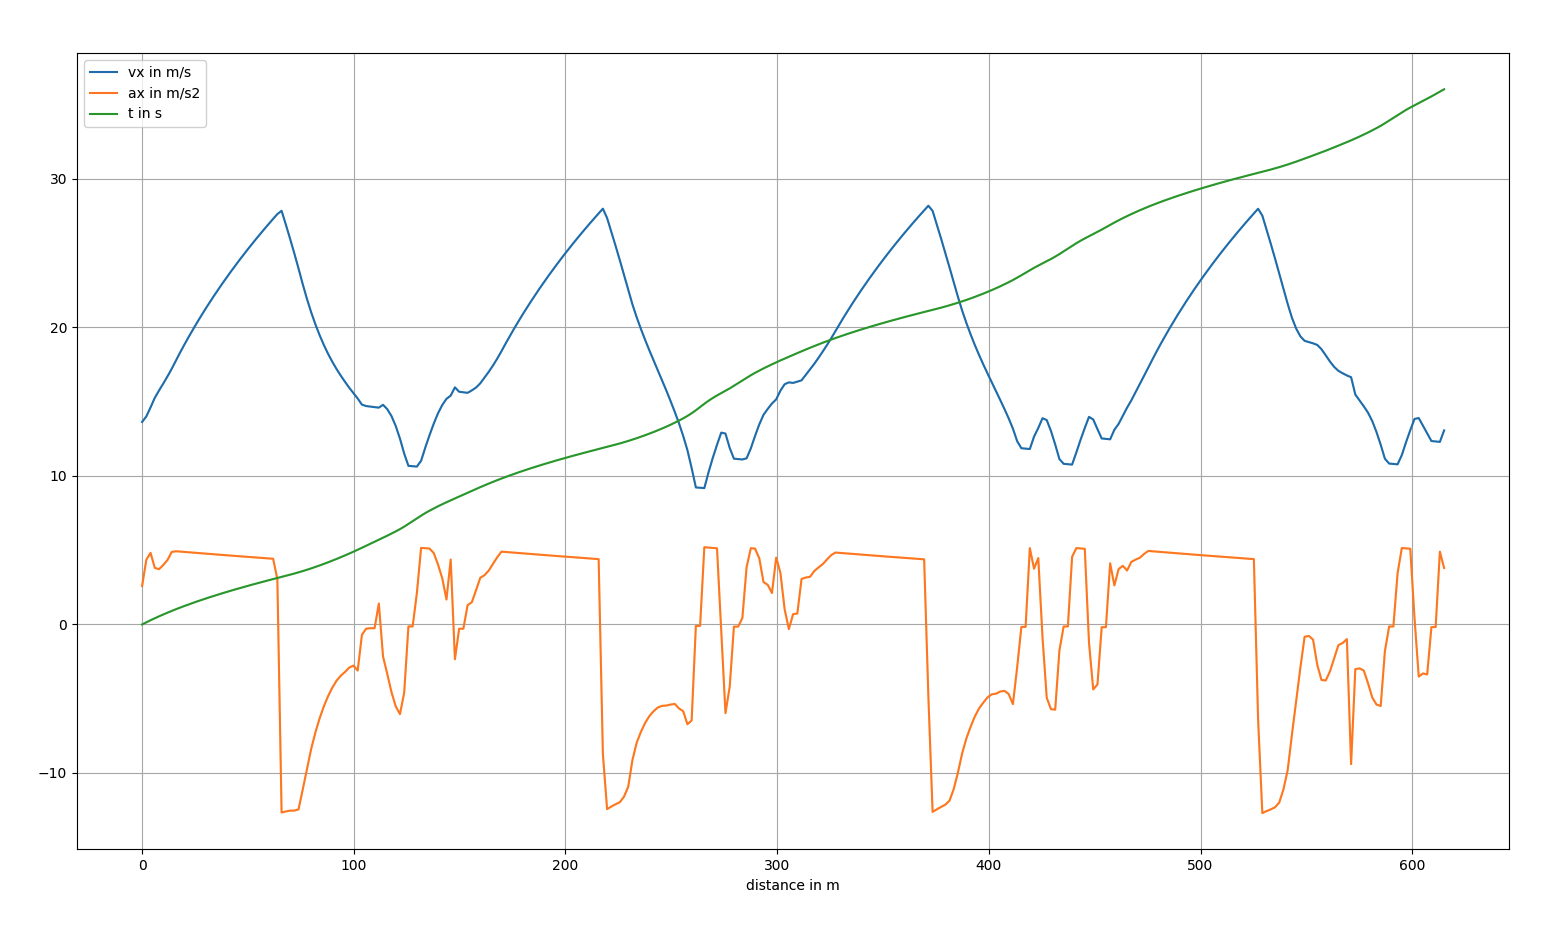
\includegraphics[width=\columnwidth]{Results_Optimization_Rounded_Rectangle_Laps_2_VelAcc_Profile.png}
    \caption{The Velocity and Acceleration Profile on Rounded Rectangle track for two laps.}
    \label{fig:Results Rounded Rectangle Laps 2 VelAcc Profile}
\end{figure}
\begin{figure}[H]
    \centering
    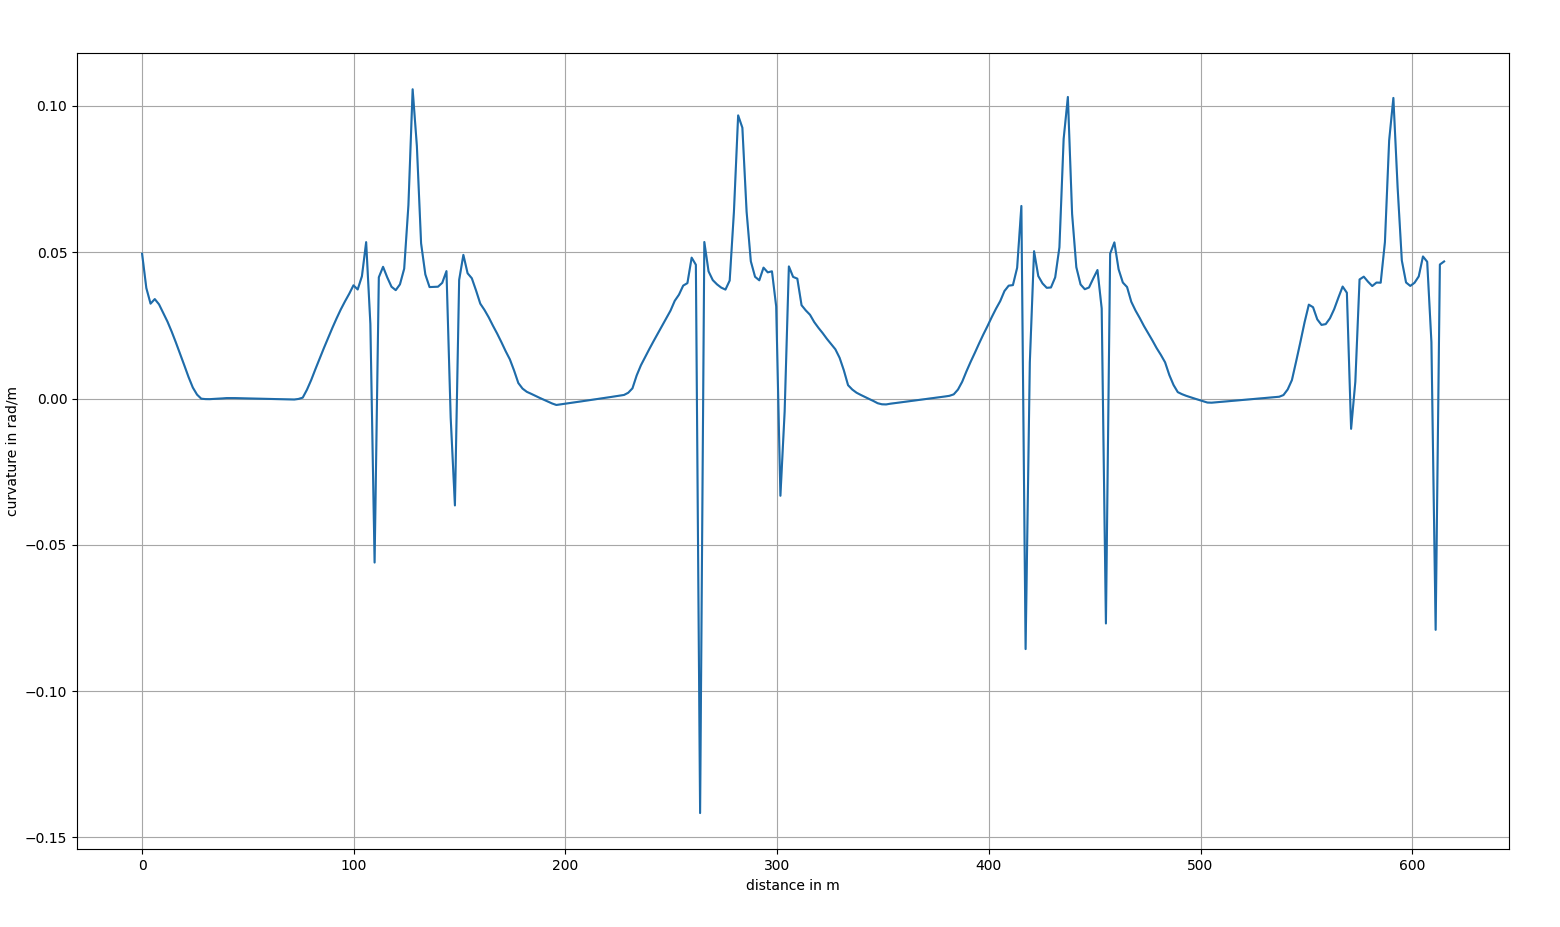
\includegraphics[width=\columnwidth]{Results_Optimization_Rounded_Rectangle_Laps_2_Curv_Profile.png}
    \caption{The Curvature Profile on the Rounded Rectangle track for two laps.}
    \label{fig:Results Rounded Rectangle Laps 2 Curv Profile}
\end{figure}
\begin{figure}[H]
    \centering
    \includegraphics[width=\columnwidth]{Results_Optimization_Rounded_Rectangle_Laps_2_Spline_Normals.png}
    \caption{The Spline Normals on the Rounded Rectangle track for two laps.}
    \label{fig:Results Rounded Rectangle Laps 2 Spline Normals}
\end{figure}

\section{Handling Track} \label{sec:Results Handling Track}
The track was created by \acrshort{tumftm} and was provided together with the ``global\_racetrajectory\_optimization'' repository. \cite{tumftm_optimization_algoritm}
As the track information came already in the format which would be generated by the 'Optimization Input Transformer' described in section \ref{sec:Optimization Input Transformer}, the track could only be tested with the Optimization Algorithm, but not with the Exploration Algorithm.

\textbf{Optimization Algorithm}

A comparison of the different objectives on the Handling Track is given in table \ref{tab:Results Handling Track Optimization Objectives}. Two laps on the given track were calculated for each objective: Shortest Path, Minimum Curvature and Minimum Curvature with iterative call. The result with the Shortest Path objective is seen in figure \ref{fig:Results Handling Track Laps 2 Shortest Path}, the result with the Minimum Curvature objective is seen in figure \ref{fig:Results Handling Track Laps 2 Minimum Curvature}, and the result with the Minimum Curvature objective with an iterative call is seen in figure \ref{fig:Results Handling Track Laps 2 Minimum Curvature IQP}.

\begin{table}[H]
    \centering
    \begin{tabular}{|l|l|l|l|}
        \hline
        \textbf{Objective}    & \textbf{Runtime} & \textbf{Estimated Lap Time} & \textbf{Generated Reference Points} \\ \hline
        Shortest Path         & 1.15 s           & 74.79 s                     & 563 Reference Points                \\ \hline
        Minimum Curvature     & 1.72 s           & 71.94 s                     & 582 Reference Points                \\ \hline
        Minimum Curvature IQP & 3.59 s           & 67.95 s                     & 587 Reference Points                \\ \hline
    \end{tabular}
    \caption{Results of the different Optimization Algorithm objectives on the Handling Track for two laps.}
    \label{tab:Results Handling Track Optimization Objectives}
\end{table}
\begin{figure}[H]
    \centering
    \includegraphics[width=\columnwidth]{Results_Optimization_Handling_Track_Laps_2_Shortest_Path.png}
    \caption{Optimization on the Handling Track for two laps with the Shortest Path objective.}
    \label{fig:Results Handling Track Laps 2 Shortest Path}
\end{figure}
\begin{figure}[H]
    \centering
    \includegraphics[width=\columnwidth]{Results_Optimization_Handling_Track_Laps_2.png}
    \caption{Optimization on the Handling Track for two laps with the Minimum Curvature objective.}
    \label{fig:Results Handling Track Laps 2 Minimum Curvature}
\end{figure}
\begin{figure}[H]
    \centering
    \includegraphics[width=\columnwidth]{Results_Optimization_Handling_Track_Laps_2_Mincurv_IQP.png}
    \caption{Optimization on the Handling Track for two laps with the Minimum Curvature objective with iterative call.}
    \label{fig:Results Handling Track Laps 2 Minimum Curvature IQP}
\end{figure}

Additionally, the following outputs of the Optimization Algorithm with the Minimum Curvature objective for two laps on the Handling Track are shown: The Velocity and Acceleration Profile in figure \ref{fig:Results Handling Track Laps 2 VelAcc Profile}, the Curvature Profile in figure \ref{fig:Results Handling Track Laps 2 Curv Profile}, and the Spline Normals in figure \ref{fig:Results Handling Track Laps 2 Spline Normals}.
\begin{figure}[H]
    \centering
    \includegraphics[width=\columnwidth]{Results_Optimization_Handling_Track_Laps_2_VelAcc_Profile.png}
    \caption{The Velocity and Acceleration Profile on the Handling Track for two laps.}
    \label{fig:Results Handling Track Laps 2 VelAcc Profile}
\end{figure}
\begin{figure}[H]
    \centering
    \includegraphics[width=\columnwidth]{Results_Optimization_Handling_Track_Laps_2_Curv_Profile.png}
    \caption{The Curvature Profile on the Handling Track for two laps.}
    \label{fig:Results Handling Track Laps 2 Curv Profile}
\end{figure}
\begin{figure}[H]
    \centering
    \includegraphics[width=\columnwidth]{Results_Optimization_Handling_Track_Laps_2_Spline_Normals.png}
    \caption{The Spline Normals on the Handling Track for two laps.}
    \label{fig:Results Handling Track Laps 2 Spline Normals}
\end{figure}

\section{Berlin 2018 Track} \label{sec:Results Berlin 2018 Track}
The track was created by \acrshort{tumftm} and was provided together with the ``global\_racetrajectory\_optimization'' repository. \cite{tumftm_optimization_algoritm}
As the track information came already in the format which would be generated by the 'Optimization Input Transformer' described in section \ref{sec:Optimization Input Transformer}, the track could only be tested with the Optimization Algorithm, but not with the Exploration Algorithm. The track is a recreation of the 2018 Berlin ePrix in Formula E. \cite{formula_e_berlin_eprix}

\textbf{Optimization Algorithm}

A comparison of the different objectives on the Berlin 2018 track is given in table \ref{tab:Results Berlin 2018 Optimization Objectives}. Two laps on the given track were calculated for each objective: Shortest Path, Minimum Curvature and Minimum Curvature with iterative call. The result with the Shortest Path objective is seen in figure \ref{fig:Results Berlin 2018 Laps 2 Shortest Path}, the result with the Minimum Curvature objective is seen in figure \ref{fig:Results Berlin 2018 Laps 2 Minimum Curvature}, and the result with the Minimum Curvature objective with an iterative call is seen in figure \ref{fig:Results Berlin 2018 Laps 2 Minimum Curvature IQP}.

\begin{table}[H]
    \centering
    \begin{tabular}{|l|l|l|l|}
        \hline
        \textbf{Objective}    & \textbf{Runtime} & \textbf{Estimated Lap Time} & \textbf{Generated Reference Points} \\ \hline
        Shortest Path         & 23.03 s          & 196.57 s                    & 2272 Reference Points               \\ \hline
        Minimum Curvature     & 38.30 s          & 186.15 s                    & 2325 Reference Points               \\ \hline
        Minimum Curvature IQP & 102.86 s         & 184.00 s                    & 2322 Reference Points               \\ \hline
    \end{tabular}
    \caption{Results of the different Optimization Algorithm objectives on the Berlin 2018 track for two laps.}
    \label{tab:Results Berlin 2018 Optimization Objectives}
\end{table}
\begin{figure}[H]
    \centering
    \includegraphics[width=\columnwidth]{Results_Optimization_Berlin_2018_Laps_2_Shortest_Path.png}
    \caption{Optimization on the Berlin 2018 track for two laps with the Shortest Path objective.}
    \label{fig:Results Berlin 2018 Laps 2 Shortest Path}
\end{figure}
\begin{figure}[H]
    \centering
    \includegraphics[width=\columnwidth]{Results_Optimization_Berlin_2018_Laps_2.png}
    \caption{Optimization on the Berlin 2018 track for two laps with the Minimum Curvature objective.}
    \label{fig:Results Berlin 2018 Laps 2 Minimum Curvature}
\end{figure}
\begin{figure}[H]
    \centering
    \includegraphics[width=\columnwidth]{Results_Optimization_Berlin_2018_Laps_2_Mincurv_IQP.png}
    \caption{Optimization on the Berlin 2018 track for two laps with the Minimum Curvature objective with iterative call.}
    \label{fig:Results Berlin 2018 Laps 2 Minimum Curvature IQP}
\end{figure}

Additionally, the following outputs of the Optimization Algorithm with the Minimum Curvature objective for two laps on the Berlin 2018 track are shown: The Velocity and Acceleration Profile in figure \ref{fig:Results Berlin 2018 Laps 2 VelAcc Profile}, the Curvature Profile in figure \ref{fig:Results Berlin 2018 Laps 2 Curv Profile}, and the Spline Normals in figure \ref{fig:Results Berlin 2018 Laps 2 Spline Normals}.
\begin{figure}[H]
    \centering
    \includegraphics[width=\columnwidth]{Results_Optimization_Berlin_2018_Laps_2_VelAcc_Profile.png}
    \caption{The Velocity and Acceleration Profile on Berlin 2018 track for two laps.}
    \label{fig:Results Berlin 2018 Laps 2 VelAcc Profile}
\end{figure}
\begin{figure}[H]
    \centering
    \includegraphics[width=\columnwidth]{Results_Optimization_Berlin_2018_Laps_2_Curv_Profile.png}
    \caption{The Curvature Profile on the Berlin 2018 track for two laps.}
    \label{fig:Results Berlin 2018 Laps 2 Curv Profile}
\end{figure}
\begin{figure}[H]
    \centering
    \includegraphics[width=\columnwidth]{Results_Optimization_Berlin_2018_Laps_2_Spline_Normals.png}
    \caption{The Spline Normals on the Berlin 2018 track for two laps.}
    \label{fig:Results Berlin 2018 Laps 2 Spline Normals}
\end{figure}

\section{Modena 2019 Track} \label{sec:Results Modena 2019 Track}
The track was created by \acrshort{tumftm} and was provided together with the ``global\_racetrajectory\_optimization'' repository. \cite{tumftm_optimization_algoritm}
As the track information came already in the format which would be generated by the 'Optimization Input Transformer' described in section \ref{sec:Optimization Input Transformer}, the track could only be tested with the Optimization Algorithm, but not with the Exploration Algorithm. The track is a recreation of the Autodromo di Modena race track. \cite{modena_race_track}

\textbf{Optimization Algorithm}

A comparison of the different objectives on the Modena 2019 track is given in table \ref{tab:Results Modena 2019 Optimization Objectives}. Two laps on the given track were calculated for each objective: Shortest Path, Minimum Curvature and Minimum Curvature with iterative call. The result with the Shortest Path objective is seen in figure \ref{fig:Results Modena 2019 Laps 2 Shortest Path}, the result with the Minimum Curvature objective is seen in figure \ref{fig:Results Modena 2019 Laps 2 Minimum Curvature}, and the result with the Minimum Curvature objective with an iterative call is seen in figure \ref{fig:Results Modena 2019 Laps 2 Minimum Curvature IQP}.

\begin{table}[H]
    \centering
    \begin{tabular}{|l|l|l|l|}
        \hline
        \textbf{Objective}    & \textbf{Runtime} & \textbf{Estimated Lap Time} & \textbf{Generated Reference Points} \\ \hline
        Shortest Path         & 14.51 s          & 184.03 s                    & 1946 Reference Points               \\ \hline
        Minimum Curvature     & 26.00 s          & 171.20 s                    & 1998 Reference Points               \\ \hline
        Minimum Curvature IQP & 69.75 s          & 169.11 s                    & 1998 Reference Points               \\ \hline
    \end{tabular}
    \caption{Results of the different Optimization Algorithm objectives on the Modena 2019 track for two laps.}
    \label{tab:Results Modena 2019 Optimization Objectives}
\end{table}
\begin{figure}[H]
    \centering
    \includegraphics[width=\columnwidth]{Results_Optimization_Modena_2019_Laps_2_Shortest_Path.png}
    \caption{Optimization on the Modena 2019 track for two laps with the Shortest Path objective.}
    \label{fig:Results Modena 2019 Laps 2 Shortest Path}
\end{figure}
\begin{figure}[H]
    \centering
    \includegraphics[width=\columnwidth]{Results_Optimization_Modena_2019_Laps_2.png}
    \caption{Optimization on the Modena 2019 track for two laps with the Minimum Curvature objective.}
    \label{fig:Results Modena 2019 Laps 2 Minimum Curvature}
\end{figure}
\begin{figure}[H]
    \centering
    \includegraphics[width=\columnwidth]{Results_Optimization_Modena_2019_Laps_2_Mincurv_IQP.png}
    \caption{Optimization on the Modena 2019 track for two laps with the Minimum Curvature objective with iterative call.}
    \label{fig:Results Modena 2019 Laps 2 Minimum Curvature IQP}
\end{figure}

Additionally, the following outputs of the Optimization Algorithm with the Minimum Curvature objective for two laps on the Modena 2019 track are shown: The Velocity and Acceleration Profile in figure \ref{fig:Results Modena 2019 Laps 2 VelAcc Profile}, the Curvature Profile in figure \ref{fig:Results Modena 2019 Laps 2 Curv Profile}, and the Spline Normals in figure \ref{fig:Results Modena 2019 Laps 2 Spline Normals}.
\begin{figure}[H]
    \centering
    \includegraphics[width=\columnwidth]{Results_Optimization_Modena_2019_Laps_2_VelAcc_Profile.png}
    \caption{The Velocity and Acceleration Profile on the Modena 2019 track for two laps.}
    \label{fig:Results Modena 2019 Laps 2 VelAcc Profile}
\end{figure}
\begin{figure}[H]
    \centering
    \includegraphics[width=\columnwidth]{Results_Optimization_Modena_2019_Laps_2_Curv_Profile.png}
    \caption{The Curvature Profile on the Modena 2019 track for two laps.}
    \label{fig:Results Modena 2019 Laps 2 Curv Profile}
\end{figure}
\begin{figure}[H]
    \centering
    \includegraphics[width=\columnwidth]{Results_Optimization_Modena_2019_Laps_2_Spline_Normals.png}
    \caption{The Spline Normals on the Modena 2019 track for two laps.}
    \label{fig:Results Modena 2019 Laps 2 Spline Normals}
\end{figure}

\section{Integration}
\begin{itemize}
    \item Test im Python Plots
    \item Simulationstool (Screenshot, evtl. folge von Screenshots), welche strecke (grafik simulationstool)
\end{itemize}

